%&preformat-disser
\RequirePackage[l2tabu,orthodox]{nag} % Раскомментировав, можно в логе получать рекомендации относительно правильного использования пакетов и предупреждения об устаревших и нерекомендуемых пакетах
% Формат А4, 14pt (ГОСТ Р 7.0.11-2011, 5.3.6)
\documentclass[a4paper,14pt,oneside,openany]{memoir}

%%%%%%%%%%%%%%%%%%%%%%%%%%%%%%%%%%%%%%%%%%%%%%%%%%%%%%%%%%%%%%%%%%%%%%%%%%%%%%%%
%%%% Файл упрощённых настроек шаблона, общих для диссертации и автореферата %%%%
%%%%%%%%%%%%%%%%%%%%%%%%%%%%%%%%%%%%%%%%%%%%%%%%%%%%%%%%%%%%%%%%%%%%%%%%%%%%%%%%

%%% Режим черновика %%%
\makeatletter
\@ifundefined{c@draft}{
  \newcounter{draft}
  \setcounter{draft}{0}  % 0 --- чистовик (максимальное соблюдение ГОСТ)
                         % 1 --- черновик (отклонения от ГОСТ, но быстрая
                         %       сборка итоговых PDF)
}{}
\makeatother

%%% Пометки в тексте %%%
\makeatletter
\@ifundefined{c@showmarkup}{
  \newcounter{showmarkup}
  \setcounter{showmarkup}{0}  % 0 --- скрыть пометки
                              % 1 --- показывать пометки
}{}
\makeatother

%%% Использование в pdflatex шрифтов не по-умолчанию %%%
\makeatletter
\@ifundefined{c@usealtfont}{
  \newcounter{usealtfont}
  \setcounter{usealtfont}{1}    % 0 --- шрифты на базе Computer Modern
                                % 1 --- использовать пакет pscyr, при его
                                %       наличии
                                % 2 --- использовать пакет XCharter, при наличии
                                %       подходящей версии
}{}
\makeatother

%%% Использование в xelatex и lualatex семейств шрифтов %%%
\makeatletter
\@ifundefined{c@fontfamily}{
  \newcounter{fontfamily}
  \setcounter{fontfamily}{1}  % 0 --- CMU семейство. Используется как fallback;
                              % 1 --- Шрифты от MS (Times New Roman и компания)
                              % 2 --- Семейство Liberation
}{}
\makeatother

%%% Библиография %%%
\makeatletter
\@ifundefined{c@bibliosel}{
  \newcounter{bibliosel}
  \setcounter{bibliosel}{1}   % 0 --- встроенная реализация с загрузкой файла
                              %       через движок bibtex8;
                              % 1 --- реализация пакетом biblatex через движок
                              %       biber
}{}
\makeatother

%%% Вывод типов ссылок в библиографии %%%
\makeatletter
\@ifundefined{c@mediadisplay}{
  \newcounter{mediadisplay}
  \setcounter{mediadisplay}{0}   % 0 --- не делать ничего; надписи [Текст] и
                                 %       [Эл. ресурс] будут выводиться только в ссылках с
                                 %       заполненным полем `media`;
                                 % 1 --- автоматически добавлять надпись [Текст] к ссылкам с
                                 %       незаполненным полем `media`; таким образом, у всех
                                 %       источников будет указан тип, что соответствует
                                 %       требованиям ГОСТ
                                 % 2 --- автоматически удалять надписи [Текст], [Эл. Ресурс] и др.;
                                 %       не соответствует ГОСТ
                                 % 3 --- автоматически удалять надпись [Текст];
                                 %       не соответствует ГОСТ
                                 % 4 --- автоматически удалять надпись [Эл. Ресурс];
                                 %       не соответствует ГОСТ
}{}
\makeatother

%%% Предкомпиляция tikz рисунков для ускорения работы %%%
\makeatletter
\@ifundefined{c@imgprecompile}{
  \newcounter{imgprecompile}
  \setcounter{imgprecompile}{0}   % 0 --- без предкомпиляции;
                                  % 1 --- пользоваться предварительно
                                  %       скомпилированными pdf вместо генерации
                                  %       заново из tikz
}{}
\makeatother
            % общие настройки шаблона
\input{common/packages}         % Пакеты общие для диссертации и автореферата
\synopsisfalse                      % Этот документ --- не автореферат
\input{Dissertation/dispackages}    % Пакеты для диссертации
\usepackage{fr-longtable}    %ради \endlasthead

% Листинги с исходным кодом программ
\usepackage{fancyvrb}
\usepackage{listings}
\lccode`\~=0\relax %Без этого хака из-за особенностей пакета listings перестают работать конструкции с \MakeLowercase и т. п. в (xe|lua)latex

% Русская традиция начертания греческих букв
\usepackage{upgreek} % прямые греческие ради русской традиции

%%% Микротипографика
%\ifnumequal{\value{draft}}{0}{% Только если у нас режим чистовика
%    \usepackage[final, babel, shrink=45]{microtype}[2016/05/14] % улучшает представление букв и слов в строках, может помочь при наличии отдельно висящих слов
%}{}

% Отметка о версии черновика на каждой странице
% Чтобы работало надо в своей локальной копии по инструкции
% https://www.ctan.org/pkg/gitinfo2 создать небходимые файлы в папке
% ./git/hooks
% If you’re familiar with tweaking git, you can probably work it out for
% yourself. If not, I suggest you follow these steps:
% 1. First, you need a git repository and working tree. For this example,
% let’s suppose that the root of the working tree is in ~/compsci
% 2. Copy the file post-xxx-sample.txt (which is in the same folder of
% your TEX distribution as this pdf) into the git hooks directory in your
% working copy. In our example case, you should end up with a file called
% ~/compsci/.git/hooks/post-checkout
% 3. If you’re using a unix-like system, don’t forget to make the file executable.
% Just how you do this is outside the scope of this manual, but one
% possible way is with commands such as this:
% chmod g+x post-checkout.
% 4. Test your setup with “git checkout master” (or another suitable branch
% name). This should generate copies of gitHeadInfo.gin in the directories
% you intended.
% 5. Now make two more copies of this file in the same directory (hooks),
% calling them post-commit and post-merge, and you’re done. As before,
% users of unix-like systems should ensure these files are marked as
% executable.
\ifnumequal{\value{draft}}{1}{% Черновик
   \IfFileExists{.git/gitHeadInfo.gin}{
      \usepackage[mark,pcount]{gitinfo2}
      \renewcommand{\gitMark}{rev.\gitAbbrevHash\quad\gitCommitterEmail\quad\gitAuthorIsoDate}
      \renewcommand{\gitMarkFormat}{\rmfamily\color{Gray}\small\bfseries}
   }{}
}{}

\usepackage{blkarray}   % Пакеты для специфических пользовательских задач

%%%%%%%%%%%%%%%%%%%%%%%%%%%%%%%%%%%%%%%%%%%%%%%%%%%%%%%%%%%%%%%%%%%%%%%%%%%%%%%%
%%%% Файл упрощённых настроек шаблона, общих для диссертации и автореферата %%%%
%%%%%%%%%%%%%%%%%%%%%%%%%%%%%%%%%%%%%%%%%%%%%%%%%%%%%%%%%%%%%%%%%%%%%%%%%%%%%%%%

%%% Режим черновика %%%
\makeatletter
\@ifundefined{c@draft}{
  \newcounter{draft}
  \setcounter{draft}{0}  % 0 --- чистовик (максимальное соблюдение ГОСТ)
                         % 1 --- черновик (отклонения от ГОСТ, но быстрая
                         %       сборка итоговых PDF)
}{}
\makeatother

%%% Пометки в тексте %%%
\makeatletter
\@ifundefined{c@showmarkup}{
  \newcounter{showmarkup}
  \setcounter{showmarkup}{0}  % 0 --- скрыть пометки
                              % 1 --- показывать пометки
}{}
\makeatother

%%% Использование в pdflatex шрифтов не по-умолчанию %%%
\makeatletter
\@ifundefined{c@usealtfont}{
  \newcounter{usealtfont}
  \setcounter{usealtfont}{1}    % 0 --- шрифты на базе Computer Modern
                                % 1 --- использовать пакет pscyr, при его
                                %       наличии
                                % 2 --- использовать пакет XCharter, при наличии
                                %       подходящей версии
}{}
\makeatother

%%% Использование в xelatex и lualatex семейств шрифтов %%%
\makeatletter
\@ifundefined{c@fontfamily}{
  \newcounter{fontfamily}
  \setcounter{fontfamily}{1}  % 0 --- CMU семейство. Используется как fallback;
                              % 1 --- Шрифты от MS (Times New Roman и компания)
                              % 2 --- Семейство Liberation
}{}
\makeatother

%%% Библиография %%%
\makeatletter
\@ifundefined{c@bibliosel}{
  \newcounter{bibliosel}
  \setcounter{bibliosel}{1}   % 0 --- встроенная реализация с загрузкой файла
                              %       через движок bibtex8;
                              % 1 --- реализация пакетом biblatex через движок
                              %       biber
}{}
\makeatother

%%% Вывод типов ссылок в библиографии %%%
\makeatletter
\@ifundefined{c@mediadisplay}{
  \newcounter{mediadisplay}
  \setcounter{mediadisplay}{0}   % 0 --- не делать ничего; надписи [Текст] и
                                 %       [Эл. ресурс] будут выводиться только в ссылках с
                                 %       заполненным полем `media`;
                                 % 1 --- автоматически добавлять надпись [Текст] к ссылкам с
                                 %       незаполненным полем `media`; таким образом, у всех
                                 %       источников будет указан тип, что соответствует
                                 %       требованиям ГОСТ
                                 % 2 --- автоматически удалять надписи [Текст], [Эл. Ресурс] и др.;
                                 %       не соответствует ГОСТ
                                 % 3 --- автоматически удалять надпись [Текст];
                                 %       не соответствует ГОСТ
                                 % 4 --- автоматически удалять надпись [Эл. Ресурс];
                                 %       не соответствует ГОСТ
}{}
\makeatother

%%% Предкомпиляция tikz рисунков для ускорения работы %%%
\makeatletter
\@ifundefined{c@imgprecompile}{
  \newcounter{imgprecompile}
  \setcounter{imgprecompile}{0}   % 0 --- без предкомпиляции;
                                  % 1 --- пользоваться предварительно
                                  %       скомпилированными pdf вместо генерации
                                  %       заново из tikz
}{}
\makeatother
      % Упрощённые настройки шаблона

% Новые переменные, которые могут использоваться во всём проекте
% ГОСТ 7.0.11-2011
% 9.2 Оформление текста автореферата диссертации
% 9.2.1 Общая характеристика работы включает в себя следующие основные структурные
% элементы:
% актуальность темы исследования;
\newcommand{\actualityTXT}{Актуальность и степень разработанности темы исследования.}
% степень ее разработанности;
\newcommand{\progressTXT}{Степень разработанности темы.}
% цели и задачи;
\newcommand{\aimTXT}{Целью}
\newcommand{\tasksTXT}{задачи}
% научную новизну;
\newcommand{\noveltyTXT}{Научная новизна:}
% теоретическую и практическую значимость работы;
%\newcommand{\influenceTXT}{Теоретическая и практическая значимость}
% или чаще используют просто
\newcommand{\influenceTXT}{Практическая значимость}
% методологию и методы исследования;
\newcommand{\methodsTXT}{Методология и методы исследования.}
% положения, выносимые на защиту;
\newcommand{\defpositionsTXT}{Основные положения, выносимые на~защиту:}
% степень достоверности и апробацию результатов.
\newcommand{\reliabilityTXT}{Достоверность}
\newcommand{\probationTXT}{Апробация работы.}

\newcommand{\contributionTXT}{Личный вклад.}
\newcommand{\publicationsTXT}{Публикации.}


%%% Заголовки библиографии:

% для автореферата:
\newcommand{\bibtitleauthor}{Публикации автора по теме диссертации}

% для стиля библиографии `\insertbiblioauthorgrouped`
\newcommand{\bibtitleauthorvak}{В изданиях из списка ВАК РФ}
\newcommand{\bibtitleauthorscopus}{В изданиях, входящих в международную базу цитирования Scopus}
\newcommand{\bibtitleauthorwos}{В изданиях, входящих в международную базу цитирования Web of Science}
\newcommand{\bibtitleauthorother}{В прочих изданиях}
\newcommand{\bibtitleauthorconf}{В сборниках трудов конференций}
\newcommand{\bibtitleauthorpatent}{Зарегистрированные патенты}
\newcommand{\bibtitleauthorprogram}{Зарегистрированные программы для ЭВМ}

% для стиля библиографии `\insertbiblioauthorimportant`:
\newcommand{\bibtitleauthorimportant}{Наиболее значимые \protect\MakeLowercase\bibtitleauthor}

% для списка литературы в диссертации и списка чужих работ в автореферате:
\newcommand{\bibtitlefull}{Список литературы} % (ГОСТ Р 7.0.11-2011, 4)
         % Новые переменные, для всего проекта

%%% Основные сведения %%%
\newcommand{\thesisAuthorLastName}{Кривоносов}
\newcommand{\thesisAuthorOtherNames}{Михаил Игоревич}
\newcommand{\thesisAuthorInitials}{М.\,И.}
\newcommand{\thesisAuthor}             % Диссертация, ФИО автора
{%
    \texorpdfstring{% \texorpdfstring takes two arguments and uses the first for (La)TeX and the second for pdf
        \thesisAuthorLastName~\thesisAuthorOtherNames% так будет отображаться на титульном листе или в тексте, где будет использоваться переменная
    }{%
        \thesisAuthorLastName, \thesisAuthorOtherNames% эта запись для свойств pdf-файла. В таком виде, если pdf будет обработан программами для сбора библиографических сведений, будет правильно представлена фамилия.
    }
}
\newcommand{\thesisAuthorShort}        % Диссертация, ФИО автора инициалами
{\thesisAuthorInitials~\thesisAuthorLastName}
%\newcommand{\thesisUdk}                % Диссертация, УДК
%{xxx.xxx}
\newcommand{\thesisTitle}              % Диссертация, название
{Случайные блуждания как стратегии поиска: моделирование и оценка эффективности}
\newcommand{\thesisSpecialtyNumber}    % Диссертация, специальность, номер
{1.3.4.}
\newcommand{\thesisSpecialtyTitle}     % Диссертация, специальность, название (название взято с сайта ВАК для примера)
{Радиофизика}
%% \newcommand{\thesisSpecialtyTwoNumber} % Диссертация, вторая специальность, номер
%% {XX.XX.XX}
%% \newcommand{\thesisSpecialtyTwoTitle}  % Диссертация, вторая специальность, название
%% {\fixme{Теория и~методика физического воспитания, спортивной тренировки,
%% оздоровительной и~адаптивной физической культуры}}
\newcommand{\thesisDegree}             % Диссертация, ученая степень
{кандидата физико-математических наук}
\newcommand{\thesisDegreeShort}        % Диссертация, ученая степень, краткая запись
{канд. физ.-мат. наук}
\newcommand{\thesisCity}               % Диссертация, город написания диссертации
{Нижний Новгород}
\newcommand{\thesisYear}               % Диссертация, год написания диссертации
{\the\year}
\newcommand{\thesisOrganization}       % Диссертация, организация
{Федеральное государственное автономное образовательное учреждение высшего образования «Национальный исследовательский Нижегородский государственный университет им. Н.И. Лобачевского» (ННГУ)}
\newcommand{\thesisOrganizationShort}  % Диссертация, краткое название организации для доклада
{ННГУ им. Н.И. Лобачевского}

\newcommand{\thesisInOrganization}     % Диссертация, организация в предложном падеже: Работа выполнена в ...
{Федеральном государственном автономном образовательном учреждении высшего образования «Национальный исследовательский Нижегородский государственный университет им. Н.И. Лобачевского» (ННГУ)}

%% \newcommand{\supervisorDead}{}           % Рисовать рамку вокруг фамилии
\newcommand{\supervisorFio}              % Научный руководитель, ФИО
{Иванченко Михаил Васильевич}
\newcommand{\supervisorRegalia}          % Научный руководитель, регалии
{доктор физико-математических наук, доцент}
\newcommand{\supervisorFioShort}         % Научный руководитель, ФИО
{М.\,В.~Иванченко}
\newcommand{\supervisorRegaliaShort}     % Научный руководитель, регалии
{д.ф.-м.н.,доцент}

%% \newcommand{\supervisorTwoDead}{}        % Рисовать рамку вокруг фамилии
%% \newcommand{\supervisorTwoFio}           % Второй научный руководитель, ФИО
%% {Фамилия Имя Отчество}
%% \newcommand{\supervisorTwoRegalia}       % Второй научный руководитель, регалии
%% {уч. степень, уч. звание}
%% \newcommand{\supervisorTwoFioShort}      % Второй научный руководитель, ФИО
%% {И.\,О.~Фамилия}
%% \newcommand{\supervisorTwoRegaliaShort}  % Второй научный руководитель, регалии
%% {уч.~ст.,~уч.~зв.}

\newcommand{\opponentOneFio}           % Оппонент 1, ФИО
{\fixme{Фамилия Имя Отчество}}
\newcommand{\opponentOneRegalia}       % Оппонент 1, регалии
{\fixme{кандидат физико-математических наук}}
\newcommand{\opponentOneJobPlace}      % Оппонент 1, место работы
{\fixme{Основное место работы c длинным длинным длинным длинным названием}}
\newcommand{\opponentOneJobPost}       % Оппонент 1, должность
{\fixme{старший научный сотрудник}}

\newcommand{\opponentTwoFio}           % Оппонент 2, ФИО
{\fixme{Фамилия Имя Отчество}}
\newcommand{\opponentTwoRegalia}       % Оппонент 2, регалии
{\fixme{кандидат физико-математических наук}}
\newcommand{\opponentTwoJobPlace}      % Оппонент 2, место работы
{\fixme{Основное место работы c длинным длинным длинным длинным названием}}
\newcommand{\opponentTwoJobPost}       % Оппонент 2, должность
{\fixme{старший научный сотрудник}}

%% \newcommand{\opponentThreeFio}         % Оппонент 3, ФИО
%% {\fixme{Фамилия Имя Отчество}}
%% \newcommand{\opponentThreeRegalia}     % Оппонент 3, регалии
%% {\fixme{кандидат физико-математических наук}}
%% \newcommand{\opponentThreeJobPlace}    % Оппонент 3, место работы
%% {\fixme{Основное место работы c длинным длинным длинным длинным названием}}
%% \newcommand{\opponentThreeJobPost}     % Оппонент 3, должность
%% {\fixme{старший научный сотрудник}}







\newcommand{\leadingOrganizationTitle} % Ведущая организация, дополнительные строки. Удалить, чтобы не отображать в автореферате
{\fixme{Федеральное государственное бюджетное образовательное учреждение высшего
профессионального образования с~длинным длинным длинным длинным названием}}

\newcommand{\defenseDate}              % Защита, дата
{\fixme{DD mmmmmmmm YYYY~г.~в~XX часов}}
\newcommand{\defenseCouncilNumber}     % Защита, номер диссертационного совета
{\fixme{24.2.340.03}}
\newcommand{\defenseCouncilTitle}      % Защита, учреждение диссертационного совета
{\fixme{Название учреждения}}
\newcommand{\defenseCouncilAddress}    % Защита, адрес учреждение диссертационного совета
{\fixme{603022, г. Нижний Новгород, пр. Гагарина, 23, корп. 1, ауд. 420.}}
\newcommand{\defenseCouncilPhone}      % Телефон для справок
{\fixme{+7~(0000)~00-00-00}}

\newcommand{\defenseSecretaryFio}      % Секретарь диссертационного совета, ФИО
{\fixme{Клюев Алексей Викторович}}
\newcommand{\defenseSecretaryRegalia}  % Секретарь диссертационного совета, регалии
{\fixme{д.~ф.-м.~н.}}            % Для сокращений есть ГОСТы, например: ГОСТ Р 7.0.12-2011 + http://base.garant.ru/179724/#block_30000

\newcommand{\synopsisLibrary}          % Автореферат, название библиотеки
{\fixme{Название библиотеки}}
\newcommand{\synopsisDate}             % Автореферат, дата рассылки
{\fixme{DD mmmmmmmm}\the\year~года}

% To avoid conflict with beamer class use \providecommand
\providecommand{\keywords}%            % Ключевые слова для метаданных PDF диссертации и автореферата
{}
             % Основные сведения
\input{common/fonts}            % Определение шрифтов (частичное)
%%% Шаблон %%%
\DeclareRobustCommand{\fixme}{\textcolor{red}}  % решаем проблему превращения
                                % названия цвета в результате \MakeUppercase,
                                % http://tex.stackexchange.com/a/187930,
                                % \DeclareRobustCommand protects \fixme
                                % from expanding inside \MakeUppercase
\AtBeginDocument{%
    \setlength{\parindent}{2.5em}                   % Абзацный отступ. Должен быть одинаковым по всему тексту и равен пяти знакам (ГОСТ Р 7.0.11-2011, 5.3.7).
}

%%% Таблицы %%%
\DeclareCaptionLabelSeparator{tabsep}{\tablabelsep} % нумерация таблиц
\DeclareCaptionFormat{split}{\splitformatlabel#1\par\splitformattext#3}

\captionsetup[table]{
        format=\tabformat,                % формат подписи (plain|hang)
        font=normal,                      % нормальные размер, цвет, стиль шрифта
        skip=.0pt,                        % отбивка под подписью
        parskip=.0pt,                     % отбивка между параграфами подписи
        position=above,                   % положение подписи
        justification=\tabjust,           % центровка
        indent=\tabindent,                % смещение строк после первой
        labelsep=tabsep,                  % разделитель
        singlelinecheck=\tabsinglecenter, % не выравнивать по центру, если умещается в одну строку
}

%%% Рисунки %%%
\DeclareCaptionLabelSeparator{figsep}{\figlabelsep} % нумерация рисунков

\captionsetup[figure]{
        format=plain,                     % формат подписи (plain|hang)
        font=normal,                      % нормальные размер, цвет, стиль шрифта
        skip=.0pt,                        % отбивка под подписью
        parskip=.0pt,                     % отбивка между параграфами подписи
        position=below,                   % положение подписи
        singlelinecheck=true,             % выравнивание по центру, если умещается в одну строку
        justification=centerlast,         % центровка
        labelsep=figsep,                  % разделитель
}

%%% Подписи подрисунков %%%
\DeclareCaptionSubType{figure}
\renewcommand\thesubfigure{\asbuk{subfigure}} % нумерация подрисунков
\ifsynopsis
\DeclareCaptionFont{norm}{\fontsize{10pt}{11pt}\selectfont}
\newcommand{\subfigureskip}{2.pt}
\else
\DeclareCaptionFont{norm}{\fontsize{14pt}{16pt}\selectfont}
\newcommand{\subfigureskip}{0.pt}
\fi

\captionsetup[subfloat]{
        labelfont=norm,                 % нормальный размер подписей подрисунков
        textfont=norm,                  % нормальный размер подписей подрисунков
        labelsep=space,                 % разделитель
        labelformat=brace,              % одна скобка справа от номера
        justification=centering,        % центровка
        singlelinecheck=true,           % выравнивание по центру, если умещается в одну строку
        skip=\subfigureskip,            % отбивка над подписью
        parskip=.0pt,                   % отбивка между параграфами подписи
        position=below,                 % положение подписи
}

%%% Настройки ссылок на рисунки, таблицы и др. %%%
% команды \cref...format отвечают за форматирование при помощи команды \cref
% команды \labelcref...format отвечают за форматирование при помощи команды \labelcref

\ifpresentation
\else
    \crefdefaultlabelformat{#2#1#3}

    % Уравнение
    \crefformat{equation}{(#2#1#3)} % одиночная ссылка с приставкой
    \labelcrefformat{equation}{(#2#1#3)} % одиночная ссылка без приставки
    \crefrangeformat{equation}{(#3#1#4) \cyrdash~(#5#2#6)} % диапазон ссылок с приставкой
    \labelcrefrangeformat{equation}{(#3#1#4) \cyrdash~(#5#2#6)} % диапазон ссылок без приставки
    \crefmultiformat{equation}{(#2#1#3)}{ и~(#2#1#3)}{, (#2#1#3)}{ и~(#2#1#3)} % перечисление ссылок с приставкой
    \labelcrefmultiformat{equation}{(#2#1#3)}{ и~(#2#1#3)}{, (#2#1#3)}{ и~(#2#1#3)} % перечисление без приставки

    % Подуравнение
    \crefformat{subequation}{(#2#1#3)} % одиночная ссылка с приставкой
    \labelcrefformat{subequation}{(#2#1#3)} % одиночная ссылка без приставки
    \crefrangeformat{subequation}{(#3#1#4) \cyrdash~(#5#2#6)} % диапазон ссылок с приставкой
    \labelcrefrangeformat{subequation}{(#3#1#4) \cyrdash~(#5#2#6)} % диапазон ссылок без приставки
    \crefmultiformat{subequation}{(#2#1#3)}{ и~(#2#1#3)}{, (#2#1#3)}{ и~(#2#1#3)} % перечисление ссылок с приставкой
    \labelcrefmultiformat{subequation}{(#2#1#3)}{ и~(#2#1#3)}{, (#2#1#3)}{ и~(#2#1#3)} % перечисление без приставки

    % Глава
    \crefformat{chapter}{#2#1#3} % одиночная ссылка с приставкой
    \labelcrefformat{chapter}{#2#1#3} % одиночная ссылка без приставки
    \crefrangeformat{chapter}{#3#1#4 \cyrdash~#5#2#6} % диапазон ссылок с приставкой
    \labelcrefrangeformat{chapter}{#3#1#4 \cyrdash~#5#2#6} % диапазон ссылок без приставки
    \crefmultiformat{chapter}{#2#1#3}{ и~#2#1#3}{, #2#1#3}{ и~#2#1#3} % перечисление ссылок с приставкой
    \labelcrefmultiformat{chapter}{#2#1#3}{ и~#2#1#3}{, #2#1#3}{ и~#2#1#3} % перечисление без приставки

    % Параграф
    \crefformat{section}{#2#1#3} % одиночная ссылка с приставкой
    \labelcrefformat{section}{#2#1#3} % одиночная ссылка без приставки
    \crefrangeformat{section}{#3#1#4 \cyrdash~#5#2#6} % диапазон ссылок с приставкой
    \labelcrefrangeformat{section}{#3#1#4 \cyrdash~#5#2#6} % диапазон ссылок без приставки
    \crefmultiformat{section}{#2#1#3}{ и~#2#1#3}{, #2#1#3}{ и~#2#1#3} % перечисление ссылок с приставкой
    \labelcrefmultiformat{section}{#2#1#3}{ и~#2#1#3}{, #2#1#3}{ и~#2#1#3} % перечисление без приставки

    % Приложение
    \crefformat{appendix}{#2#1#3} % одиночная ссылка с приставкой
    \labelcrefformat{appendix}{#2#1#3} % одиночная ссылка без приставки
    \crefrangeformat{appendix}{#3#1#4 \cyrdash~#5#2#6} % диапазон ссылок с приставкой
    \labelcrefrangeformat{appendix}{#3#1#4 \cyrdash~#5#2#6} % диапазон ссылок без приставки
    \crefmultiformat{appendix}{#2#1#3}{ и~#2#1#3}{, #2#1#3}{ и~#2#1#3} % перечисление ссылок с приставкой
    \labelcrefmultiformat{appendix}{#2#1#3}{ и~#2#1#3}{, #2#1#3}{ и~#2#1#3} % перечисление без приставки

    % Рисунок
    \crefformat{figure}{#2#1#3} % одиночная ссылка с приставкой
    \labelcrefformat{figure}{#2#1#3} % одиночная ссылка без приставки
    \crefrangeformat{figure}{#3#1#4 \cyrdash~#5#2#6} % диапазон ссылок с приставкой
    \labelcrefrangeformat{figure}{#3#1#4 \cyrdash~#5#2#6} % диапазон ссылок без приставки
    \crefmultiformat{figure}{#2#1#3}{ и~#2#1#3}{, #2#1#3}{ и~#2#1#3} % перечисление ссылок с приставкой
    \labelcrefmultiformat{figure}{#2#1#3}{ и~#2#1#3}{, #2#1#3}{ и~#2#1#3} % перечисление без приставки

    % Таблица
    \crefformat{table}{#2#1#3} % одиночная ссылка с приставкой
    \labelcrefformat{table}{#2#1#3} % одиночная ссылка без приставки
    \crefrangeformat{table}{#3#1#4 \cyrdash~#5#2#6} % диапазон ссылок с приставкой
    \labelcrefrangeformat{table}{#3#1#4 \cyrdash~#5#2#6} % диапазон ссылок без приставки
    \crefmultiformat{table}{#2#1#3}{ и~#2#1#3}{, #2#1#3}{ и~#2#1#3} % перечисление ссылок с приставкой
    \labelcrefmultiformat{table}{#2#1#3}{ и~#2#1#3}{, #2#1#3}{ и~#2#1#3} % перечисление без приставки

    % Листинг
    \crefformat{lstlisting}{#2#1#3} % одиночная ссылка с приставкой
    \labelcrefformat{lstlisting}{#2#1#3} % одиночная ссылка без приставки
    \crefrangeformat{lstlisting}{#3#1#4 \cyrdash~#5#2#6} % диапазон ссылок с приставкой
    \labelcrefrangeformat{lstlisting}{#3#1#4 \cyrdash~#5#2#6} % диапазон ссылок без приставки
    \crefmultiformat{lstlisting}{#2#1#3}{ и~#2#1#3}{, #2#1#3}{ и~#2#1#3} % перечисление ссылок с приставкой
    \labelcrefmultiformat{lstlisting}{#2#1#3}{ и~#2#1#3}{, #2#1#3}{ и~#2#1#3} % перечисление без приставки

    % Листинг
    \crefformat{ListingEnv}{#2#1#3} % одиночная ссылка с приставкой
    \labelcrefformat{ListingEnv}{#2#1#3} % одиночная ссылка без приставки
    \crefrangeformat{ListingEnv}{#3#1#4 \cyrdash~#5#2#6} % диапазон ссылок с приставкой
    \labelcrefrangeformat{ListingEnv}{#3#1#4 \cyrdash~#5#2#6} % диапазон ссылок без приставки
    \crefmultiformat{ListingEnv}{#2#1#3}{ и~#2#1#3}{, #2#1#3}{ и~#2#1#3} % перечисление ссылок с приставкой
    \labelcrefmultiformat{ListingEnv}{#2#1#3}{ и~#2#1#3}{, #2#1#3}{ и~#2#1#3} % перечисление без приставки
\fi

%%% Настройки гиперссылок %%%
\ifluatex
    \hypersetup{
        unicode,                % Unicode encoded PDF strings
    }
\fi

\hypersetup{
    linktocpage=true,           % ссылки с номера страницы в оглавлении, списке таблиц и списке рисунков
%    linktoc=all,                % both the section and page part are links
%    pdfpagelabels=false,        % set PDF page labels (true|false)
    plainpages=false,           % Forces page anchors to be named by the Arabic form  of the page number, rather than the formatted form
    colorlinks,                 % ссылки отображаются раскрашенным текстом, а не раскрашенным прямоугольником, вокруг текста
    linkcolor={linkcolor},      % цвет ссылок типа ref, eqref и подобных
    citecolor={citecolor},      % цвет ссылок-цитат
    urlcolor={urlcolor},        % цвет гиперссылок
%    hidelinks,                  % Hide links (removing color and border)
    pdftitle={\thesisTitle},    % Заголовок
    pdfauthor={\thesisAuthor},  % Автор
    pdfsubject={\thesisSpecialtyNumber\ \thesisSpecialtyTitle},      % Тема
%    pdfcreator={Создатель},     % Создатель, Приложение
%    pdfproducer={Производитель},% Производитель, Производитель PDF
    pdfkeywords={\keywords},    % Ключевые слова
    pdflang={ru}
}
\ifnumequal{\value{draft}}{1}{% Черновик
    \hypersetup{
        draft,
    }
}{}

%%% Списки %%%
% Используем короткое тире (endash) для ненумерованных списков (ГОСТ 2.105-95, пункт 4.1.7, требует дефиса, но так лучше смотрится)
\renewcommand{\labelitemi}{\normalfont\bfseries{--}}

% Перечисление строчными буквами латинского алфавита (ГОСТ 2.105-95, 4.1.7)
%\renewcommand{\theenumi}{\alph{enumi}}
%\renewcommand{\labelenumi}{\theenumi)}

% Перечисление строчными буквами русского алфавита (ГОСТ 2.105-95, 4.1.7)
\makeatletter
\AddEnumerateCounter{\asbuk}{\russian@alph}{щ}      % Управляем списками/перечислениями через пакет enumitem, а он 'не знает' про asbuk, потому 'учим' его
\makeatother
%\renewcommand{\theenumi}{\asbuk{enumi}} %первый уровень нумерации
%\renewcommand{\labelenumi}{\theenumi)} %первый уровень нумерации
\renewcommand{\theenumii}{\asbuk{enumii}} %второй уровень нумерации
\renewcommand{\labelenumii}{\theenumii)} %второй уровень нумерации
\renewcommand{\theenumiii}{\arabic{enumiii}} %третий уровень нумерации
\renewcommand{\labelenumiii}{\theenumiii)} %третий уровень нумерации

\setlist{nosep,%                                    % Единый стиль для всех списков (пакет enumitem), без дополнительных интервалов.
    labelindent=\parindent,leftmargin=*%            % Каждый пункт, подпункт и перечисление записывают с абзацного отступа (ГОСТ 2.105-95, 4.1.8)
}

%%% Правильная нумерация приложений, рисунков и формул %%%
%% По ГОСТ 2.105, п. 4.3.8 Приложения обозначают заглавными буквами русского алфавита,
%% начиная с А, за исключением букв Ё, З, Й, О, Ч, Ь, Ы, Ъ.
%% Здесь также переделаны все нумерации русскими буквами.
\ifxetexorluatex
    \makeatletter
    \def\russian@Alph#1{\ifcase#1\or
       А\or Б\or В\or Г\or Д\or Е\or Ж\or
       И\or К\or Л\or М\or Н\or
       П\or Р\or С\or Т\or У\or Ф\or Х\or
       Ц\or Ш\or Щ\or Э\or Ю\or Я\else\xpg@ill@value{#1}{russian@Alph}\fi}
    \def\russian@alph#1{\ifcase#1\or
       а\or б\or в\or г\or д\or е\or ж\or
       и\or к\or л\or м\or н\or
       п\or р\or с\or т\or у\or ф\or х\or
       ц\or ш\or щ\or э\or ю\or я\else\xpg@ill@value{#1}{russian@alph}\fi}
    \def\cyr@Alph#1{\ifcase#1\or
        А\or Б\or В\or Г\or Д\or Е\or Ж\or
        И\or К\or Л\or М\or Н\or
        П\or Р\or С\or Т\or У\or Ф\or Х\or
        Ц\or Ш\or Щ\or Э\or Ю\or Я\else\xpg@ill@value{#1}{cyr@Alph}\fi}
    \def\cyr@alph#1{\ifcase#1\or
        а\or б\or в\or г\or д\or е\or ж\or
        и\or к\or л\or м\or н\or
        п\or р\or с\or т\or у\or ф\or х\or
        ц\or ш\or щ\or э\or ю\or я\else\xpg@ill@value{#1}{cyr@alph}\fi}
    \makeatother
\else
    \makeatletter
    \if@uni@ode
      \def\russian@Alph#1{\ifcase#1\or
        А\or Б\or В\or Г\or Д\or Е\or Ж\or
        И\or К\or Л\or М\or Н\or
        П\or Р\or С\or Т\or У\or Ф\or Х\or
        Ц\or Ш\or Щ\or Э\or Ю\or Я\else\@ctrerr\fi}
    \else
      \def\russian@Alph#1{\ifcase#1\or
        \CYRA\or\CYRB\or\CYRV\or\CYRG\or\CYRD\or\CYRE\or\CYRZH\or
        \CYRI\or\CYRK\or\CYRL\or\CYRM\or\CYRN\or
        \CYRP\or\CYRR\or\CYRS\or\CYRT\or\CYRU\or\CYRF\or\CYRH\or
        \CYRC\or\CYRSH\or\CYRSHCH\or\CYREREV\or\CYRYU\or
        \CYRYA\else\@ctrerr\fi}
    \fi
    \if@uni@ode
      \def\russian@alph#1{\ifcase#1\or
        а\or б\or в\or г\or д\or е\or ж\or
        и\or к\or л\or м\or н\or
        п\or р\or с\or т\or у\or ф\or х\or
        ц\or ш\or щ\or э\or ю\or я\else\@ctrerr\fi}
    \else
      \def\russian@alph#1{\ifcase#1\or
        \cyra\or\cyrb\or\cyrv\or\cyrg\or\cyrd\or\cyre\or\cyrzh\or
        \cyri\or\cyrk\or\cyrl\or\cyrm\or\cyrn\or
        \cyrp\or\cyrr\or\cyrs\or\cyrt\or\cyru\or\cyrf\or\cyrh\or
        \cyrc\or\cyrsh\or\cyrshch\or\cyrerev\or\cyryu\or
        \cyrya\else\@ctrerr\fi}
    \fi
    \makeatother
\fi


%%http://www.linux.org.ru/forum/general/6993203#comment-6994589 (используется totcount)
\makeatletter
\def\formtotal#1#2#3#4#5{%
    \newcount\@c
    \@c\totvalue{#1}\relax
    \newcount\@last
    \newcount\@pnul
    \@last\@c\relax
    \divide\@last 10
    \@pnul\@last\relax
    \divide\@pnul 10
    \multiply\@pnul-10
    \advance\@pnul\@last
    \multiply\@last-10
    \advance\@last\@c
    #2%
    \ifnum\@pnul=1#5\else%
    \ifcase\@last#5\or#3\or#4\or#4\or#4\else#5\fi
    \fi
}
\makeatother

\newcommand{\formbytotal}[5]{\total{#1}~\formtotal{#1}{#2}{#3}{#4}{#5}}

%%% Команды рецензирования %%%
\ifboolexpr{ (test {\ifnumequal{\value{draft}}{1}}) or (test {\ifnumequal{\value{showmarkup}}{1}})}{
        \newrobustcmd{\todo}[1]{\textcolor{red}{#1}}
        \newrobustcmd{\note}[2][]{\ifstrempty{#1}{#2}{\textcolor{#1}{#2}}}
        \newenvironment{commentbox}[1][]%
        {\ifstrempty{#1}{}{\color{#1}}}%
        {}
}{
        \newrobustcmd{\todo}[1]{}
        \newrobustcmd{\note}[2][]{}
        \excludecomment{commentbox}
}
           % Стили общие для диссертации и автореферата
\input{Dissertation/disstyles}  % Стили для диссертации
\input{Dissertation/userstyles} % Стили для специфических пользовательских задач

%%% Библиография. Выбор движка для реализации %%%
% Здесь только проверка установленного ключа. Сама настройка выбора движка
% размещена в common/setup.tex
\ifnumequal{\value{bibliosel}}{0}{%
    %%% Реализация библиографии встроенными средствами посредством движка bibtex8 %%%

%%% Пакеты %%%
\usepackage{cite}                                   % Красивые ссылки на литературу


%%% Стили %%%
\bibliographystyle{BibTeX-Styles/utf8gost71u}    % Оформляем библиографию по ГОСТ 7.1 (ГОСТ Р 7.0.11-2011, 5.6.7)

\makeatletter
\renewcommand{\@biblabel}[1]{#1.}   % Заменяем библиографию с квадратных скобок на точку
\makeatother
%% Управление отступами между записями
%% требует etoolbox
%% http://tex.stackexchange.com/a/105642
%\patchcmd\thebibliography
% {\labelsep}
% {\labelsep\itemsep=5pt\parsep=0pt\relax}
% {}
% {\typeout{Couldn't patch the command}}

%%% Список литературы с красной строки (без висячего отступа) %%%
%\patchcmd{\thebibliography} %может потребовать включения пакета etoolbox
%  {\advance\leftmargin\labelsep}
%  {\leftmargin=0pt%
%   \setlength{\labelsep}{\widthof{\ }}% Управляет длиной отступа после точки
%   \itemindent=\parindent%
%   \addtolength{\itemindent}{\labelwidth}% Сдвигаем правее на величину номера с точкой
%   \advance\itemindent\labelsep%
%  }
%  {}{}

%%% Цитирование %%%
\renewcommand\citepunct{;\penalty\citepunctpenalty%
    \hskip.13emplus.1emminus.1em\relax}                % Разделение ; при перечислении ссылок (ГОСТ Р 7.0.5-2008)

\newcommand*{\autocite}[1]{}  % Чтобы примеры цитирования, рассчитанные на biblatex, не вызывали ошибок при компиляции в bibtex

%%% Создание команд для вывода списка литературы %%%
\newcommand*{\insertbibliofull}{
\bibliography{biblio/external,biblio/author,biblio/registered}         % Подключаем BibTeX-базы % После запятых не должно быть лишних пробелов — он "думает", что это тоже имя пути
}

\newcommand*{\insertbiblioauthor}{
\bibliography{biblio/author,biblio/registered}         % Подключаем BibTeX-базы % После запятых не должно быть лишних пробелов — он "думает", что это тоже имя пути
}

\newcommand*{\insertbiblioexternal}{
\bibliography{biblio/external}         % Подключаем BibTeX-базы
}


%% Счётчик использованных ссылок на литературу, обрабатывающий с учётом неоднократных ссылок
%% Требуется дважды компилировать, поскольку ему нужно считать актуальный внешний файл со списком литературы
\newtotcounter{citenum}
\def\oldcite{}
\let\oldcite=\bibcite
\def\bibcite{\stepcounter{citenum}\oldcite}
   % Встроенная реализация с загрузкой файла через движок bibtex8
}{
    \input{biblio/biblatex}     % Реализация пакетом biblatex через движок biber
}

% Вывести информацию о выбранных опциях в лог сборки
\typeout{Selected options:}
\typeout{Draft mode: \arabic{draft}}
\typeout{Font: \arabic{fontfamily}}
\typeout{AltFont: \arabic{usealtfont}}
\typeout{Bibliography backend: \arabic{bibliosel}}
\typeout{Precompile images: \arabic{imgprecompile}}
% Вывести информацию о версиях используемых библиотек в лог сборки
\listfiles

%%% Управление компиляцией отдельных частей диссертации %%%
% Необходимо сначала иметь полностью скомпилированный документ, чтобы все
% промежуточные файлы были в наличии
% Затем, для вывода отдельных частей можно воспользоваться командой \includeonly
% Ниже примеры использования команды:
%
%\includeonly{Dissertation/part2}
%\includeonly{Dissertation/contents,Dissertation/appendix,Dissertation/conclusion}
%
% Если все команды закомментированы, то документ будет выведен в PDF файл полностью

\begin{document}
%%% Переопределение именований типовых разделов
% https://tex.stackexchange.com/a/156050
\gappto\captionsrussian{\input{common/renames}\unskip} % for polyglossia and babel
\input{common/renames}

%%% Структура диссертации (ГОСТ Р 7.0.11-2011, 4)
% Титульный лист (ГОСТ Р 7.0.11-2001, 5.1)
\thispagestyle{empty}
\begin{center}
\thesisOrganization
\end{center}
%
\vspace{0pt plus4fill} %число перед fill = кратность относительно некоторого расстояния fill, кусками которого заполнены пустые места
\IfFileExists{images/logo.pdf}{
  \begin{minipage}[b]{0.5\linewidth}
    \begin{flushleft}
      
\includegraphics[height=5.5cm]{images/logo.pdf}
    \end{flushleft}
  \end{minipage}%
  \begin{minipage}[b]{0.5\linewidth}
    \begin{flushright}
      На правах рукописи\\
%      \textsl {УДК \thesisUdk}
    \end{flushright}
  \end{minipage}
}{
\begin{flushright}
На правах рукописи

%\textsl {УДК \thesisUdk}
\end{flushright}
}
%
\vspace{0pt plus6fill} %число перед fill = кратность относительно некоторого расстояния fill, кусками которого заполнены пустые места
\begin{center}
{\large \thesisAuthor}
\end{center}
%
\vspace{0pt plus1fill} %число перед fill = кратность относительно некоторого расстояния fill, кусками которого заполнены пустые места
\begin{center}
\textbf {\large %\MakeUppercase
\thesisTitle}

\vspace{0pt plus2fill} %число перед fill = кратность относительно некоторого расстояния fill, кусками которого заполнены пустые места
{%\small
Специальность \thesisSpecialtyNumber\ "---

<<\thesisSpecialtyTitle>>
}

\ifdefined\thesisSpecialtyTwoNumber
{%\small
Специальность \thesisSpecialtyTwoNumber\ "---

<<\thesisSpecialtyTwoTitle>>
}
\fi

\vspace{0pt plus2fill} %число перед fill = кратность относительно некоторого расстояния fill, кусками которого заполнены пустые места
Диссертация на соискание учёной степени

\thesisDegree
\end{center}
%
\vspace{0pt plus4fill} %число перед fill = кратность относительно некоторого расстояния fill, кусками которого заполнены пустые места
\begin{flushright}
\ifdefined\supervisorTwoFio
Научные руководители:

\supervisorRegalia

\ifdefined\supervisorDead
\framebox{\supervisorFio}
\else
\supervisorFio
\fi

\supervisorTwoRegalia

\ifdefined\supervisorTwoDead
\framebox{\supervisorTwoFio}
\else
\supervisorTwoFio
\fi
\else
Научный руководитель:

\supervisorRegalia

\ifdefined\supervisorDead
\framebox{\supervisorFio}
\else
\supervisorFio
\fi
\fi

\end{flushright}
%
\vspace{0pt plus4fill} %число перед fill = кратность относительно некоторого расстояния fill, кусками которого заполнены пустые места
{\centering\thesisCity\ "--- \thesisYear\par}
           % Титульный лист
\include{Dissertation/contents}        % Оглавление
\ifnumequal{\value{contnumfig}}{1}{}{\counterwithout{figure}{chapter}}
\ifnumequal{\value{contnumtab}}{1}{}{\counterwithout{table}{chapter}}
\chapter*{Введение}                         % Заголовок
\addcontentsline{toc}{chapter}{Введение}    % Добавляем его в оглавление

\newcommand{\actuality}{\textbf\actualityTXT}
\newcommand{\progress}{}
\newcommand{\aim}{{\textbf\aimTXT}}
\newcommand{\tasks}{\textbf{\tasksTXT}}
\newcommand{\novelty}{\textbf{\noveltyTXT}}
\newcommand{\influence}{\textbf{\influenceTXT}}
\newcommand{\methods}{\textbf{\methodsTXT}}
\newcommand{\defpositions}{\textbf{\defpositionsTXT}}
\newcommand{\reliability}{\textbf{\reliabilityTXT}}
\newcommand{\probation}{\textbf{\probationTXT}}
\newcommand{\contribution}{\textbf{\contributionTXT}}
\newcommand{\publications}{\textbf{\publicationsTXT}}


{\actuality} <<Игровые>> взаимодействия, в которых каждый участник руководствуется принципами максимизации выигрыша в некоторой игре -- 
либо своего личного, либо целого коллектива («популяции») – существенно отличны от обычных физических взаимодействий. 
Дополненные механизмами обучения, оценки и адаптации, игровые взаимодействия определяют принципиально новый тип динамики или <<эволюции>> [1]. 
К настоящему времени стало понятно, что область применения игровой динамики гораздо шире социологии и экологии, и что соответствующие 
методы могут быть использованы для моделирования динамики финансовых рынков [2] и интерпретации процессов Бозе-Эйнштейн конденсации в открытых квантовых системах [3]. 

Объект исследования данной работы — процессы случайных блужданий, обусловленные конфликтным взаимодействием игроков. 
Модельный процесс представляет собой игру, в которой игроки управляют перемещением точки (индикатор положения) на квадратной решетке, 
делая независимый выбор одной из двух возможных стратегий (<<ход>>) на каждом шаге игры. Информация о возможных перемещениях точки 
(определяемых совместным выбором), открыта для обоих игроков и организована в виде матрицы. Целью первого игрока является максимально 
долгое удержание точки внутри ограниченной области, а второго -- максимально быстрое достижение ею поглощающей границы. 
Результатом игры («платежом») является время поглощения. 

Игры такого типа были определены в некоторых работах по теории игр и принятия решений еще в 1950-1960х годах [4,5]. 
Однако, в силу вычислительной сложности задачи, количественные результаты были получены только для очень простых моделей 
с тремя-пятью состояниями [6], что не позволяет делать заключения об асимптотических характеристиках процесса и использовать 
для их анализа статистический подход. Существует тесная связь между «играми на выживание» и процессами случайных блужданий, 
например, классическая задача о разорении игрока допускает прямую интерпретацию как процесс случайного блуждания на конечном интервале [6]. 

С другой стороны, проблема случайных блужданий в ограниченной области и такие вопросы, как оценка среднего времени достижения границы 
(или любого другого определённого региона). [7], в настоящее время испытывает очередную волну интереса, вызванную перспективами 
приложения этого подхода к проблемам молекулярной биологии, химической кинетики, и экологии [8-9]. 

Идея данной работы состоит в том, что игровые <<блуждания>> в конечных пространственных областях, ограниченных поглощающими границами 
(достижение границы является выигрышем одного из игроков и, соответственно, проигрышем его оппонента), 
могут быть исследованы и квантифицированы, используя методологию теории случайных блужданий. Более конкретно, 
предлагается исследовать распределение времени достижения границы (<<времени игры>>). Очевидно, что такое распределение 
будет существенно отличаться от распределения времени достижения границ для стандартных моделей случайных блужданий 
в той же ограниченной области [8]. Одна из задач -- построение стохастической модели, которая бы воспроизводила это распределение. 
В работе проводится сравнение теоретических результатов с экспериментальными данными, собранными c помощью мобильного приложения. 
Следует отметить, что использование методик таких экспериментов (в областях далеких от социологии, где, главным образом, эта методика локализована) 
является одним из новейших трендов в области прикладной математики и математического моделирования; см., например [10-12].
Данная работа предполагает проведение масштабного «полевого эксперимента» с участием реальных игроков. 
Таким образом, область исследований лежит на стыке трех областей: теории случайных блужданий, теории игр и принятия решений 
и технологии социальных экспериментов с использованием мобильных приложений. 

В соответствии с паспортом специальности 05.13.18 <<Математическое моделирование,
численные методы и комплексы программ>>, данная диссертация
относится к следующим областям исследований: <<3. Разработка, обоснование
и тестирование эффективных вычислительных методов с применением современных
компьютерных технологий>>, <<4. Реализация эффективных численных методов и алгоритмов в виде
комплексов проблемно-ориентированных программ для проведения
вычислительного эксперимента>> <<5. Комплексные исследования научных и
технических проблем с применением современной технологии математического
моделирования и вычислительного эксперимента>>, <<7. Разработка новых математических
методов и алгоритмов интерпретации натурного эксперимента на
основе его математической модели>>, <<8. Разработка систем компьютерного и имитационного моделирования>>.

\ifsynopsis
Этот абзац появляется только в~автореферате.
Для формирования блоков, которые будут обрабатываться только в~автореферате,
заведена проверка условия \verb!\!\verb!ifsynopsis!.
Значение условия задаётся в~основном файле документа (\verb!synopsis.tex! для
автореферата).
\else
Этот абзац появляется только в~диссертации.
Через проверку условия \verb!\!\verb!ifsynopsis!, задаваемого в~основном файле
документа (\verb!dissertation.tex! для диссертации), можно сделать новую
команду, обеспечивающую появление цитаты в~диссертации, но~не~в~автореферате.
\fi

% {\progress}
% Этот раздел должен быть отдельным структурным элементом по
% ГОСТ, но он, как правило, включается в описание актуальности
% темы. Нужен он отдельным структурынм элемементом или нет ---
% смотрите другие диссертации вашего совета, скорее всего не нужен.

{\aim} данной работы является получение информации о статистических
характеристиках процесса блужданий в ограниченной двухмерной области, индуцированного игровым
взаимодействием двух игроков-оппонентов и построение стохастической модели, способной воспроизвести эти характеристики. 

Для~достижения поставленной цели необходимо было решить следующие {\tasks} диссертационного исследования:
\begin{enumerate}[beginpenalty=10000] % https://tex.stackexchange.com/a/476052/104425
    \item Разработка стохастической модели блужданий на плоскости, управляемых
    игровым конфликтом, и получение характеристик игрового процесса.
    \item Разработка и имплементация алгоритмов для моделирования
    игровой пространственной динамики, используя стохастическую
    модель, получение информации о статистических характеристиках
    модельного процесса, таких как время достижения границы и его
    распределение.
    \item Реализация масштабной серии экспериментов с участием
    реальных игроков и получение статистически значимого массива
    данных.
    \item Исследование взаимосвязи результатов, полученных в ходе
    теоретического анализа, численного моделирования, и эксперимента, а
    также их совместная интерпретация.
\end{enumerate}


{\novelty}
В работе получены следующие новые научные результаты:
\begin{enumerate}[beginpenalty=10000] % https://tex.stackexchange.com/a/476052/104425
  \item Впервые предложен игровой конфликт двух игроков, управляющих блужданием фишки на плоскости, реализованный в виде мобильного приложения.
        Новизна подхода заключается в применении интернет-технологий для реализации игры одновременно учитывающей как 
        возможность создания игрового взаимодействия между игроками, так и процесса случайного блуждания.
  \item Впервые разработана стохастическая модель предложенной игровой динамики, позволяющая получить характеристики игрового процесса 
        и воспроизвести результаты масштабного эксперимента игр полученных реальными игроками. Новизна подхода состоит в возможности 
        исследования модельного процесса случайного блуждания, позволяющего воспроизвести экспериментально полученные характеристики,
        а также провести точное сравнение модели с полевым экспериментом.
  \item Разработаны и реализованы численные методы для расчета статистических характеристик игрового процесса при фиксированных заданных стратегиях игроков,
        таких как среднее время игры, распределение времен игры, распределение вероятностей наблюдения фишки в состояниях конечной решетки. 
  \item Выдвинута гипотеза об оптимальном среднем времени оптимальных стратегий для двух случаев игры против стратегии случайного равновероятного выбора, продемонстрирована
        оптимальность данных значений для малых размеров игрового поля и предложены классы стратегий, достигающие предполагаемой оптимальной оценки.
\end{enumerate}

%{\influence} \ldots

{\methods} 
В работе используются методы математического моделирования, теории игр, теории вероятностей, математической статистики, 
теории Марковских цепей, теории случайных блужданий, математического программирования, численного моделирования. 
Дополнительно используется подход к проведению масштабного полевого эксперимента с применением интернет-технологий и мобильных приложений.


{\defpositions}
\begin{enumerate}[beginpenalty=10000] % https://tex.stackexchange.com/a/476052/104425
  \item Построена стохастическая модель, описывающая игровой конфликт двух игроков, управляющих блужданием фишки на конечной квадратной решетке.
  \item Созданы методы для расчета статистических характеристик игрового процесса при фиксированных заданных стратегиях игроков,
        таких как среднее время игры, распределение времен игры, распределение вероятностей наблюдения фишки в состояниях конечной решетки. 
  \item Выдвинута гипотеза об оптимальном среднем времени для двух случаев игры против стратегии случайного равновероятного выбора,
        и установлена оптимальность данных значений для малых размеров игрового поля, а также найден класс стратегий, достигающих предполагаемой оптимальной оценки.
  \item Обнаружено соответствие эксперимента предложенной модели и установлены возникающие особенности синхронизации игроков, 
        а также выявлены отличия стратегий игроков от предполагаемых оптимальных стратегий
        на основе сравнения статистических свойств траекторий и стратегий участников масштабного эксперимента, 
        проведенного с применением мобильных и интернет-технологий.
  
\end{enumerate}

{\reliability} полученных результатов, научных положений и выводов,
полученных в диссертации, обеспечивается корректным обоснованием
постановок задач, точной формулировкой критериев, подтверждается результатами
вычислительных экспериментов по использованию предложенных в
диссертации методов и алгоритмов, сравнением полученных результатов с
проведёнными ранее исследованиями и перекрестной проверкой с применением трех различных методов.
Результаты находятся в соответствии с результатами, полученными другими авторами.

{\probation}
Основные результаты диссертационного исследования докладывались~на следующих научных конференциях и фестивалях:
\begin{itemize}
    \item XXVI научная конференция по радиофизике, посвященная 120-летию со дня рождения М.Т. Греховой. 2022, ННГУ им. Н.И. Лобачевского,
    Нижний Новгород.
    \item Всероссийский фестиваль молодежных инноваций Иннофест. 2020, ННГУ им. Н.И. Лобачевского,
    Нижний Новгород.
\end{itemize}


{\contribution} Решение задач диссертационного исследования, разработка стохастической модели, описывающей игровой конфликт двух игроков,
построение и реализация методов для расчета статистических характеристик, разработка гипотезы об оптимальном среднем времени игры
для двух случаев игры против стратегии случайного равновероятного выбора принадлежат автору лично.
Разработка мобильного приложения, разработка серверной части платформы, организация масштабного эксперимента 
и сопутствующих мероприятий выполнены при непосредственном активном участии автора.
Автор принимал прямое участие в постановке задач и анализе полученных результатов, а также в подготовке публикаций
в научных журналах и докладов на тематических конференциях.

\ifnumequal{\value{bibliosel}}{0}
{%%% Встроенная реализация с загрузкой файла через движок bibtex8. (При желании, внутри можно использовать обычные ссылки, наподобие `\cite{vakbib1,vakbib2}`).
    {\publications} Основные результаты по теме диссертации изложены
    в~2~печатных изданиях,
    0 из которых изданы в журналах, рекомендованных ВАК,
    1 "--- в тезисах докладов.
}%
{%%% Реализация пакетом biblatex через движок biber
    \begin{refsection}[bl-author, bl-registered]
        % Это refsection=1.
        % Процитированные здесь работы:
        %  * подсчитываются, для автоматического составления фразы "Основные результаты ..."
        %  * попадают в авторскую библиографию, при usefootcite==0 и стиле `\insertbiblioauthor` или `\insertbiblioauthorgrouped`
        %  * нумеруются там в зависимости от порядка команд `\printbibliography` в этом разделе.
        %  * при использовании `\insertbiblioauthorgrouped`, порядок команд `\printbibliography` в нём должен быть тем же (см. biblio/biblatex.tex)
        %
        % Невидимый библиографический список для подсчёта количества публикаций:
        \printbibliography[heading=nobibheading, section=1, env=countauthorvak,          keyword=biblioauthorvak]%
        \printbibliography[heading=nobibheading, section=1, env=countauthorwos,          keyword=biblioauthorwos]%
        \printbibliography[heading=nobibheading, section=1, env=countauthorscopus,       keyword=biblioauthorscopus]%
        \printbibliography[heading=nobibheading, section=1, env=countauthorconf,         keyword=biblioauthorconf]%
        \printbibliography[heading=nobibheading, section=1, env=countauthorother,        keyword=biblioauthorother]%
        \printbibliography[heading=nobibheading, section=1, env=countregistered,         keyword=biblioregistered]%
        \printbibliography[heading=nobibheading, section=1, env=countauthorpatent,       keyword=biblioauthorpatent]%
        \printbibliography[heading=nobibheading, section=1, env=countauthorprogram,      keyword=biblioauthorprogram]%
        \printbibliography[heading=nobibheading, section=1, env=countauthor,             keyword=biblioauthor]%
        \printbibliography[heading=nobibheading, section=1, env=countauthorvakscopuswos, filter=vakscopuswos]%
        \printbibliography[heading=nobibheading, section=1, env=countauthorscopuswos,    filter=scopuswos]%
        %
        \nocite{*}%
        %
        {\publications} Основные результаты по теме диссертации изложены в~\arabic{citeauthor}~печатных изданиях,
        \arabic{citeauthorvak} из которых изданы в журналах, рекомендованных ВАК\sloppy%
        \ifnum \value{citeauthorscopuswos}>0%
            , \arabic{citeauthorscopuswos} "--- в~периодических научных журналах, индексируемых Web of~Science и Scopus\sloppy%
        \fi%
        \ifnum \value{citeauthorconf}>0%
            , \arabic{citeauthorconf} "--- в~тезисах докладов.
        \else%
            .
        \fi%
        \ifnum \value{citeregistered}=1%
            \ifnum \value{citeauthorpatent}=1%
                Зарегистрирован \arabic{citeauthorpatent} патент.
            \fi%
            \ifnum \value{citeauthorprogram}=1%
                Зарегистрирована \arabic{citeauthorprogram} программа для ЭВМ.
            \fi%
        \fi%
        \ifnum \value{citeregistered}>1%
            Зарегистрированы\ %
            \ifnum \value{citeauthorpatent}>0%
            \formbytotal{citeauthorpatent}{патент}{}{а}{}\sloppy%
            \ifnum \value{citeauthorprogram}=0 . \else \ и~\fi%
            \fi%
            \ifnum \value{citeauthorprogram}>0%
            \formbytotal{citeauthorprogram}{программ}{а}{ы}{} для ЭВМ.
            \fi%
        \fi%
        % К публикациям, в которых излагаются основные научные результаты диссертации на соискание учёной
        % степени, в рецензируемых изданиях приравниваются патенты на изобретения, патенты (свидетельства) на
        % полезную модель, патенты на промышленный образец, патенты на селекционные достижения, свидетельства
        % на программу для электронных вычислительных машин, базу данных, топологию интегральных микросхем,
        % зарегистрированные в установленном порядке.(в ред. Постановления Правительства РФ от 21.04.2016 N 335)
    \end{refsection}%
    \begin{refsection}[bl-author, bl-registered]
        % Это refsection=2.
        % Процитированные здесь работы:
        %  * попадают в авторскую библиографию, при usefootcite==0 и стиле `\insertbiblioauthorimportant`.
        %  * ни на что не влияют в противном случае
        \nocite{vakbib2}%vak
        \nocite{patbib1}%patent
        \nocite{progbib1}%program
        \nocite{bib1}%other
        \nocite{confbib1}%conf
    \end{refsection}%
        %
        % Всё, что вне этих двух refsection, это refsection=0,
        %  * для диссертации - это нормальные ссылки, попадающие в обычную библиографию
        %  * для автореферата:
        %     * при usefootcite==0, ссылка корректно сработает только для источника из `external.bib`. Для своих работ --- напечатает "[0]" (и даже Warning не вылезет).
        %     * при usefootcite==1, ссылка сработает нормально. В авторской библиографии будут только процитированные в refsection=0 работы.
}

Результаты также направлены в 1 печатное издание в журнал Chaos (IF=3.741, Manuscript ID: CHA22-AR-00995), индексируемый
в Web of Science и Scopus, в котором получены положительные
рецензии, на данный момент вносятся коррективы в соответствии
с комментариями рецензетов. Также направлена заявка на регистрацию РИД
<<Программа для моделирования эволюции вероятности и 
расчета среднего времени поглощения в антагонистической игре двух игроков, управляющих 
случайным блужданием на решетке>>.

% При использовании пакета \verb!biblatex! будут подсчитаны все работы, добавленные
% в файл \verb!biblio/author.bib!. Для правильного подсчёта работ в~различных
% системах цитирования требуется использовать поля:
% \begin{itemize}
%         \item \texttt{authorvak} если публикация индексирована ВАК,
%         \item \texttt{authorscopus} если публикация индексирована Scopus,
%         \item \texttt{authorwos} если публикация индексирована Web of Science,
%         \item \texttt{authorconf} для докладов конференций,
%         \item \texttt{authorpatent} для патентов,
%         \item \texttt{authorprogram} для зарегистрированных программ для ЭВМ,
%         \item \texttt{authorother} для других публикаций.
% \end{itemize}
% Для подсчёта используются счётчики:
% \begin{itemize}
%         \item \texttt{citeauthorvak} для работ, индексируемых ВАК,
%         \item \texttt{citeauthorscopus} для работ, индексируемых Scopus,
%         \item \texttt{citeauthorwos} для работ, индексируемых Web of Science,
%         \item \texttt{citeauthorvakscopuswos} для работ, индексируемых одной из трёх баз,
%         \item \texttt{citeauthorscopuswos} для работ, индексируемых Scopus или Web of~Science,
%         \item \texttt{citeauthorconf} для докладов на конференциях,
%         \item \texttt{citeauthorother} для остальных работ,
%         \item \texttt{citeauthorpatent} для патентов,
%         \item \texttt{citeauthorprogram} для зарегистрированных программ для ЭВМ,
%         \item \texttt{citeauthor} для суммарного количества работ.
% \end{itemize}
% % Счётчик \texttt{citeexternal} используется для подсчёта процитированных публикаций;
% % \texttt{citeregistered} "--- для подсчёта суммарного количества патентов и программ для ЭВМ.

% Для добавления в список публикаций автора работ, которые не были процитированы в
% автореферате, требуется их~перечислить с использованием команды \verb!\nocite! в
% \verb!Synopsis/content.tex!. % Характеристика работы по структуре во введении и в автореферате не отличается (ГОСТ Р 7.0.11, пункты 5.3.1 и 9.2.1), потому её загружаем из одного и того же внешнего файла, предварительно задав форму выделения некоторым параметрам

\textbf{Объем и структура работы.} Диссертация состоит из~введения,
\formbytotal{totalchapter}{глав}{ы}{}{} и
заключения. 
% \formbytotal{totalappendix}{приложен}{ия}{ий}{}.
%% на случай ошибок оставляю исходный кусок на месте, закомментированным
%Полный объём диссертации составляет  \ref*{TotPages}~страницу
%с~\totalfigures{}~рисунками и~\totaltables{}~таблицами. Список литературы
%содержит \total{citenum}~наименований.
%
Полный объем диссертации составляет
\formbytotal{TotPages}{страниц}{у}{ы}{}, включая
\formbytotal{totalcount@figure}{рисун}{ок}{ка}{ков} и
\formbytotal{totalcount@table}{таблиц}{у}{ы}{}.
Список литературы содержит
\formbytotal{citenum}{наименован}{ие}{ия}{ий}.
    % Введение
\ifnumequal{\value{contnumfig}}{1}{\counterwithout{figure}{chapter}
}{\counterwithin{figure}{chapter}}
\ifnumequal{\value{contnumtab}}{1}{\counterwithout{table}{chapter}
}{\counterwithin{table}{chapter}}
\chapter{Обзор предметной области}\label{ch:ch1}

\section{Антагонистические игры и случайные блуждания}\label{sec:ch1/sec1}

Теория игр тесно переплетается с проблемами случайных блужданий в широком спектре областей прикладных и фундаментальных исследований 
от хемотаксиса бактерий и рыночных взаимодействий до блужданий роя автономных роботов и компьютерных игр \cite{}. 
Игры, в которых возникают случай влияет на развитие игровой ситуации, могут быть рассмотрены как случайное блуждание
на некотором графе всех возможных конфигураций предметов игры или в некотором непрерывном пространстве всех возможных состояний.
В общем случае окончание таких игр определяется при возникновении некоторой предопределенной выигрышной траектории.
Одной из таких возможных ситуаций является поглощение траектории в некотором состоянии при случайном блуждании в пространстве конфигураций.
В зависимости от типа игры игрокам может требоваться оптимизировать длительность случайного блуждания или расставить поглощающие состояния 
так, чтобы раньше другого игрока поймать траекторию \cite{}. Одной из самых простых игр такого типа является задача о разорении игрока \cite{}
и различные её модификации \cite{}. Обобщение случайных блужданий игрового типа было проведено в работе И.~В.~Романовского \cite{romanovskiy_1961}.
Рассматриваемые теорией игр процессы обусловлены взаимодействием одного игрока с некоторой системой, двух игроков или множества игроков.
В последующих разделах проведен анализ первых двух случаев, соответствующих антагонистическим играм между двумя игроками с противоположными интересами.

\subsection{Задача о разорении игрока}\label{subsec:ch1/sec1/sub1}

Впервые упоминание о задаче разорения игрока появилось в переписке Блеза Паскаля и Пьера Ферма в 1656 году при рассмотрении игры тремя костями между двумя игроками.
Первый игрок получал очки при выпадении суммы на игральных костях равной 11, а второй игрок при выпадении суммы равной 14. Однако, способ начисления очков 
был модифицирован: очко добавляется к счету игрока только в том случае, если счет его противника равен нулю, а в противном случае очко будет вычтено из счета его противника.
В этом случае счет отстающего игрока всегда остается равным нулю. Первый из игроков набравший 12 очков объявлялся победителем. В переформулированной версии
письма Пьером де Каркави, направленной Христиану Гюйгенсу в 1656 году, вопрос к задаче состоял в нахождении вероятности победы первого и второго игрока. 

В своей работе De ratiociniis in ludo aleae Христиан Гюйгенс получил более приближенную формулировку к классической: игроки начинают с 12 очков, успешный бросок 
трех костей (11 для первого и 14 для второго) добавляет этому игроку одно очко и вычитает у второго, при этом первый достигший нуля очков проигрывает.
Вопрос как и ранее состоял в нахождении вероятности победы игроков. 

Классическая формулировка обобщает для одномерного случая задачу о разорении игрока для случая произвольных начальных условий и произвольных вероятностей перехода. 
Пусть у первого игрока есть $-A$ монет ($A < 0, -A > 0$), у второго игрока - $B$ монет. На каждом ходу подбрасывается ассиметричная монета, имеющая вероятность выпадения 
аверса $p$ и реверса $1-p$. При выпадении аверса одна монета переходит от второго игрока к первому, при выпадении реверса - наоборот. Требуется найти вероятность проигрыша 
за $n$ шагов, а также общую вероятность проигрыша каждого из игроков. В дополнение к формулировке Христиана Гюйгенса ставится вопрос о среднем времени игры, 
где время игры характеризует количество ходов до проигрыша одного из игроков.

Тесная связь со случайными блужданиями позволяет сформулировать данный процесс в виде дискретного блуждания частицы по целочисленному отрезку $[A; B]$, 
при этом выход на границу отрезка характеризует проигрыш одного из игроков. 

Решение задачи состоит в рассмотрении схемы Бернулли с последовательностью Бернуллиевских случайных величин $\xi_i$ с вероятностью $p$ дающих $+1$ и 
с вероятностью $q=1-p$ значение $-1$.
Тогда сумма таких величин $S_k=\sum_{i=1}^{k} \xi_i$ равна случайной величине, соответствующей положению частицы в случайном блуждании на отрезке $[A; B]$.
Вводя обозначения для вероятностей завершить игру в точках $A$ и $B$ за время $[0; k]$ при старте в позиции $x$ соответственно $\alpha_k(x), \beta_k(x)$ 
запишем рекуррентные соотношения:

\begin{equation}
    \label{eq:eq1}
    \begin{alignedat}{2}
        \alpha_k(x) = p\alpha_{k-1}(x+1)+q\alpha_{k-1}(x-1),\\
        \beta_k(x) = p\beta_{k-1}(x+1)+q\beta_{k-1}(x-1).
    \end{alignedat}
\end{equation}

При достаточно больших $n$ решение рекуррентного соотношения близко к стационарной точке точечного отображения при заданных граничных условиях:
\begin{equation}
    \label{eq:eq2}
    \begin{alignedat}{2}
        \alpha(x) = p\alpha(x+1)+q\alpha(x-1), \alpha(A)=1, \alpha(B)=0,\\
        \beta(x) = p\beta(x+1)+q\beta(x-1), \beta(A)=0, \beta(B)=1.
    \end{alignedat}
\end{equation}

Поиск решения уравнения в форме $(q/p)^{x}$ дает следующий результат:
\begin{equation}
    \label{eq:eq2}
    \begin{alignedat}{2}
        \alpha(x) = ((q/p)^B-(q/p)^x)/((q/p)^B-(q/p)^A),\\
        \beta(x) = ((q/p)^x-(q/p)^A)/((q/p)^B-(q/p)^A).
    \end{alignedat}
\end{equation}

При справедливой игре $(p=q)$ выражения для определения вероятностей редуцируются до линейной формы:
\begin{equation}
    \label{eq:eq2}
    \begin{alignedat}{2}
        \alpha(x) = (B-x)/(B-A),\\
        \beta(x) = (x-A)/(B-A),
    \end{alignedat}
\end{equation}
где $x \in [A; B]$ --- стартовое положение на отрезке.

Заключительный аспект задачи о разорении игрока состоит в исследовании среднего времени достижения финального состояния.
С точки зрения случайных блужданий процесс представляется в виде Марковской цепи с поглощающими состояниями на концах отрезка 
и промежуточными состояниями в целочисленных координатах отрезка. Рассмотрим подход к решению задачи о нахождении математического
ожидания времени окончания игры $m_k(x)$ для некоторой игры длины $k$ находящейся в состоянии $x$. Тогда рекуррентное соотношение 
для соседних состояний представляется в виде:
\begin{equation}
    \label{eq:eq2}
    m_k(x) = p m_{k-1}(x + 1) + q m_{k-1}(x - 1) + 1, x \in (A, B), k > 0,
\end{equation}

На границе в точках $A$, $B$ количество ходов для завершения игры равно нулю, то есть $m_k(A) = m_k(B) = 0$.
С учетом конечности математического ожидания пределом при $k->\infty$ будет являться решение рекуррентного соотношения 
$m(x)=p m(x+1) +q m(x - 1) + 1$. Итоговое решение для общего случая представляется в виде:

\begin{equation}
    \label{eq:eq2}
    m(x) = 1 / (p - q) (B \beta(x) + A \alpha(x) - x)
\end{equation}

При симметричной монетке формула упрощается до $m(x) = (B - x) (x - A)$, а в случае равного начального капитала $m(x) = B^2$.

Таким образом оценки позволяют найти как вероятность выигрыша каждого из игроков в зависимости от параметров игры, так и среднее время игры.

\subsection{Задача о разорении игрока с несколькими валютами}\label{subsec:ch1/sec1/sub2}

Обобщение задачи о разорении игрока на двумерный случай было рассмотрено израильскими математиками в 1994 году \cite{}. 
Для решения задачи был применен метод производящих функций и получены выражения для случая с равновероятными переходами на отрезке и на квадратной решетке.
Применяя символьные вычисления в пакете MAPLE \cite{} тем же способом было найдено решение с произвольными вероятностями перехода в 4 направлениях 
на четырех-связной решетке. 

Естественным продолжением двумерного случая является обобщение на произвольные размерности. В 2000 году Марко Петковсек и Андреем Кмет 
рассмотрели задачу о разорении игрока, в которой имеется несколько различных валют. \cite{}
Формулировка игровой механики для многомерного случая состоит в равновероятном выборе валюты и победителя на каждом ходу.
В результате хода победитель забирает одну монету выпавшей валюты у проигравшего. Игра продолжается до тех пор, пока у одного из игроков не закончатся монеты любой из валют.
В своей работе словенские математики получили среднее время игры в явной форме для случая равновероятных переходов между соседними узлами решетки
с применением дискретного преобразования Фурье и выражений для спектра симметричной тридиагональной матрицы Теплица.
Полученное выражение для среднего времени игры в зависимости от начального капитала игроков состоит из двойной суммы для двумерного случая 
и может быть вычислено за время $O(N^2)$: 
\begin{equation}
    \label{eq:eq2}
    a_{ij} = 4 / N^2 \sum_{k=1\\ k odd}^{N - 1} sin(jk\pi/N)cot(k\pi/(2N)) \sum_{l=1\\ l odd}^{N - 1} sin(il\pi/N)cot(l\pi/(2N))/(sin^2(k\pi/(2N))+sin^2(l\pi/(2N))),
    0 <= i, j <= N
\end{equation}
Хотя авторы не получили более быстрый алгоритм для общего случая, высказано предположение о возможности получения выражения в виде одной суммы.
Явные формулы в виде одной суммы (вычислительная сложность $O(N)$) были получены для частного случая стартовых капиталов одинакового размера являющегося степенью 2.
Также математики получили решение для многомерного случая на базе уравнения Сильвестра и тензорного спектрального разложения.

\subsection{Случайные блуждания}\label{subsec:ch1/sec1/sub3}

Первое появление термина "случайные блуждания" относится к письму Карла Пирсона в редакцию журнала Nature в 1905 году \cite{}.
Мотивированный проблемами, возникшими в биологии, он сформулировал следующую задачу:
"Человек начинает путешествие из точки O и проходит l ярдов по прямой линии. 
Затем он поворачивается на какой угодно угол, и проходит еще l ярдов по прямой линии. 
Он повторяет этот процесс n раз. Я ищу вероятность того, что после этих n прогулок он окажется 
на расстоянии между r и r+dr от своей начальной точки O."

На письмо ответил британский физик Лорд Рэлей, который ранее в своей работы 1880 года от теории звука рассмотрел
n изопериодических колебаний единичной амплитуды и фазы, распределенные случайным образом. Для достаточно больших n 
Рэлей нашёл асимптотическое решение в замкнутой форме, отражающее распределение вероятностей в задаче Карла Пирсона. 

Решение задачи для многомерного случая в евклидовом пространстве представляется существенно более сложной задачей в связи с чем в своих работах Лорд Рэлей
рассматривал модель случайного блуждания на решетке. Исследуя случайные блуждания на решетке Дьёрдь Пойа в своих работах 1919 и 1921 года \cite{} показал, что, 
в случае случайного блуждания на решетке с равновероятными переходами во всех направлениях в одномерном и двумерном случаях, 
агент возвращается в исходную точку с вероятностью 1, а для размерностей больше двух с вероятностью 0.

Как заметил профессор прикладной математики Невилл Темперлей, различные комбинаторные задачи, возникающие при изучении 
разнообразных физических явлений, связанных с решетками, могут быть разрешимы в терминах подсчета числа траекторий случайного блуждания с ограничениями \cite{}. 
Задачи, возникающие в различных областях таких как химия, физика, экономика, биология, сводились к анализу случайных блужданий на решетках со сложной структурой и 
особыми ограничениями \cite{, , , ...}. 

После публикации Куна в начале 20-го века все большее внимание уделялось статистике конфигураций гибких макромолекул. 
Важность исследования состояла в том, что химические свойства и биологически функции различных макромолекул напрямую 
зависят от их трехмерной пространственной конфигурации. Кун рассматривал первое приближение такой задачи 
с помощью свободно сочлененной цепи с звеньями фиксированной длины, но со случайной ориентацией, то есть задача Пирсона, но в трехмерном случае. 
Такая конструкция не учитывает тот факт, что в одной точке пространства может быть только один атом полимерной цепи. 
Упрощение задачи на случай решеток, подобно тому, как это делал Лорд Рэлей, позволяет получить решение с помощью численных методов.

Первые попытки в направлении исследования блужданий без самопересечений были сделаны В. Орром в 1946 году [61]. 
В 1924 году немецкий и американский математик Эрнст Изинг сформулировал модель ферромагнетизма на плоскости, 
для которой интересным является её соответствие случайным блужданиям без самопересечений на решетке [62]. 
В 1941 году Бартель Леендерт ван дер Варден показал, как можно свести эту задачу к подсчету числа решетчатых графов, 
состоящих из замкнутых многоугольников [63]. Знаменитое решение задачи Изинга, полученное Ларсом Онзагером, было впервые 
опубликовано 18 февраля 1942 года в дискуссионных заметках на собрании Нью-Йоркской академии наук [64]. 
Модель Изинга может быть использована для описания и других различных физических систем, таких как поглощение 
газа поверхностью или описание двухкомпонентного сплава. Эти явления описываются грубой моделью равновесия жидкости и пара на двумерной решетке.

В 1912 году Андрей Андреевич Марков разработал общую постановку задачи случайных полетов, а также предложил метод для отыскания решения [68]. 
Задача формулируется так: есть частица в трехмерном пространстве, которая совершает перемещения на каждому шаге в соответствии с некоторым распределением, 
зависящим от номера шага. Требуется найти вероятность обнаружить частицу на некотором расстоянии от позиции старта. 
Решение Маркова использует свойства преобразования Фурье.

Исследуя свойства случайных процессов в своей работе 1907 года выделил класс обладающий характеристикой независимости 
будущих состояний от прошлых состояний при определенном настоящем состоянии. В зависимости от рассматриваемой модели 
Марковские процессы могут быть обобщены на процессы с дискретным и непрерывным временем. Марковские цепи высшего порядка
в свою очередь обладают свойством зависимости перехода от последних $k$ состояний.

Анализ различных типов случайных блужданий позволил выделить множество различных объектов, на которых возможно осуществлять блуждание:
графы, числовая прямая (целые или действительные числа), векторные пространства, конечные группы, группы Ли, кривые поверхности и другие.
Случайные блуждания также различаются по типу времени: дискретное или непрерывное $(t \in [0; +\infty])$. 
Хотя в общем случае случайное блуждание не обязательно должно обладать свойством Марковости, 
по умолчанию подразумевают зависимость будущих состояний только от текущего состояния.

\subsection{Случайные блуждания игрового типа}\label{subsec:ch1/sec1/sub4}

Дальнейшие исследования игр привели к анализу многошаговых процессов, в которых игроки на каждом ходу выбирают одну из доступных стратегий \cite{}. 
Ричард Беллман в своей работе 1954 года рассматривал проблему принятия решений в многошаговых играх в условиях неопределенности \cite{} и 
привел приближенное решение задачи. Возникновение прямого конфликта позволяет использовать известные работы игр с нулевой суммой \cite{}, 
тогда как частичное противостояние требует более сложного анализа игр с ненулевой суммой \cite{}. Одной из естественно возникающих вариаций 
являются игры на выживание введенные в работах \cite{,} в 1952 году Мелвином Хауснером и Мелвином Пейсахов. В таких многошаговых схемах игроки обладают ограниченным ресурсом, 
по иссякании которого происходит завершение игры. В зависимости от количества начального числа монет оценивалась вероятность 
победы одного из игроков при некоторых фиксированных смешанных стратегиях игроков, определяемых до начала игры. Беллман показал, что в игре с нулевой суммой 
при достаточно большом стартовом капитале с большим числом ходов оптимальная стратегия игрока приблизительно такая же, как и в случае
одношаговой игры, в которой оба игрока максимизируют математическое ожидание выигрыша. 

Несмотря на полученный успех в нахождении приближенного решения многошаговой игры, требовался дальнейший анализ оптимальных стратегий. 
Используя теорию семимартингалов американские математики Ллойд Шепли и Джон Милнор в своей работе "Об играх на выживание" в 1957 году \cite{}
продемонстрировали решение функционального уравнения многошаговой игры на выживание. 

Игровая динамика многошаговых схем предполагает возможность принятия решения игроками на каждом ходу, однако в варианте Беллмана
имеет строго детерминированный исход при сделанных выборах игроков. Романовский И.В. указал на возможность обобщения игры с учетом влияния
случайной компоненты на выигрыш игроков в каждом ходе \cite{}. В работе рассмотрены различные варианты игры: игра с постоянной суммой, 
игра с бесконечным капиталом одного из игроков, и многомерные блуждания. Для различных типов игр были предложены решения функционального уравнения, 
как для вероятности победы игрока, так и для среднего времени игры.

\subsection{Мобильные приложения в полевых экспериментах}\label{subsec:ch1/sec1/sub5}

Аналитические работы математиков по теории игр построили фундаментальные основы для игровых процессов и позволили найти решение к некоторым классам игр.
Развитие вычислительной техники и рост производительности позволил решать задачи не только на бумаге проводя сложный анализ функциональных уравнений,
но и применяя принципы численного моделирования и симуляции Монте-Карло \cite{} для решения задач фиксированной размерности с конкретными значениями параметров.
Появление интернета в 1983 году создало фундамент для построения взаимодействия между большим количеством людей независимо от их географического расположения.
Внедрение цифровой мобильной связи GSM, ее эволюция и широкое внедрение по всему миру привело к возникновению технологий взаимодействия между пользователями
посредством текстовых сообщений, аудио сообщений, видео сообщений, обмена файлами, а также посредством игровых вселенных с одновременным вовлечением 
нескольких игроков. Появление возможности создания и распространения мобильных приложений среди пользователей стало новой вехой в развитии методологии
полевых экспериментов. Стандартизация процесса взаимодействия пользователей при проведении эксперимента, расширение охвата участников, получение 
объективных данных, а также более удобное воспроизведение и модификация эксперимента --- являются преимуществами использования мобильных приложений \cite{https://doi.org/10.1177/2050157917725550}.
В работе американских ученых университета Калифорнии проведен обзор 101 статей, в которых использовались мобильные приложения для проведения экспериментов.
Исследование показало, что применение приложений в полевых экспериментов началось ориентировочно с 2013 года. Большая часть приложений (77\%) были разработаны
в области исследования здравоохранения с 2013 по 2017 год. \cite{https://doi.org/10.1177/2050157917725550}

Применение мобильных приложений распространено при анализе принятия решений людьми в разных сферах жизни: 
экономике \cite{https://journals.plos.org/plosone/article?id=10.1371/journal.pone.0250668},
здравоохранении \cite{https://doi.org/10.1016/j.pmedr.2015.08.005},
мониторинге эффективности программ обучения \cite{https://doi.org/10.1007/978-981-15-7234-0_38} и других.




\section{Random Walk Game}\label{sec:ch1/sec2}

\subsection{Описание игры}\label{subsec:ch1/sec2/sub1}

\subsection{Мобильное приложение}\label{subsec:ch1/sec2/sub2}

\section{Алгоритмы и методы}\label{sec:ch1/sec3}

\subsection{Марковские цепи}\label{subsec:ch1/sec3/sub1}

\subsection{Поглощающие Марковские цепи}\label{subsec:ch1/sec3/sub2}
\subsection{Моделирование эволюции вероятности}\label{subsec:ch1/sec3/sub3}
\subsection{Численное моделирование}\label{subsec:ch1/sec3/sub4}
\subsection{Метод Монте-Карло}\label{subsec:ch1/sec3/sub5}
\subsection{Полевой эксперимент}\label{subsec:ch1/sec3/sub6}

\section{Задачи, решаемые в диссертационном исследовании}\label{sec:ch1/sec4}

\section{Выводы по главе}\label{sec:ch1/sec5}

















Мы можем сделать \textbf{жирный текст} и \textit{курсив}.

\section{Ссылки}\label{sec:ch1/sec2}

Сошлёмся на библиографию.
Одна ссылка: \cite[с.~54]{Sokolov}\cite[с.~36]{Gaidaenko}.
Две ссылки: \cite{Sokolov,Gaidaenko}.
Ссылка на собственные работы: \cite{vakbib1, confbib2}.
Много ссылок: %\cite[с.~54]{Lermontov,Management,Borozda} % такой «фокус»
%вызывает biblatex warning относительно опции sortcites, потому что неясно, к
%какому источнику относится уточнение о страницах, а bibtex об этой проблеме
%даже не предупреждает
\cite{Lermontov, Management, Borozda, Marketing, Constitution, FamilyCode,
    Gost.7.0.53, Razumovski, Lagkueva, Pokrovski, Methodology, Berestova,
    Kriger}%
\ifnumequal{\value{bibliosel}}{0}{% Примеры для bibtex8
    \cite{Sirotko, Lukina, Encyclopedia, Nasirova}%
}{% Примеры для biblatex через движок biber
    \cite{Sirotko2, Lukina2, Encyclopedia2, Nasirova2}%
}%
.
И~ещё немного ссылок:~\cite{Article,Book,Booklet,Conference,Inbook,Incollection,Manual,Mastersthesis,
    Misc,Phdthesis,Proceedings,Techreport,Unpublished}
% Следует обратить внимание, что пробел после запятой внутри \cite{}
% обрабатывается ожидаемо, а пробел перед запятой, может вызывать проблемы при
% обработке ссылок.
\cite{medvedev2006jelektronnye, CEAT:CEAT581, doi:10.1080/01932691.2010.513279,
    Gosele1999161,Li2007StressAnalysis, Shoji199895, test:eisner-sample,
    test:eisner-sample-shorted, AB_patent_Pomerantz_1968, iofis_patent1960}%
\ifnumequal{\value{bibliosel}}{0}{% Примеры для bibtex8
}{% Примеры для biblatex через движок biber
    \cite{patent2h, patent3h, patent2}%
}%
.

\ifnumequal{\value{bibliosel}}{0}{% Примеры для bibtex8
Попытка реализовать несколько ссылок на конкретные страницы
для \texttt{bibtex} реализации библиографии:
[\citenum{Sokolov}, с.~54; \citenum{Gaidaenko}, с.~36].
}{% Примеры для biblatex через движок biber
Несколько источников (мультицитата):
% Тут специально написано по-разному тире, для демонстрации, что
% применение специальных тире в настоящий момент в biblatex приводит к непоказу
% "с.".
\cites[vii--x, 5, 7]{Sokolov}[v"--~x, 25, 526]{Gaidaenko}[vii--x, 5, 7]{Techreport},
работает только в \texttt{biblatex} реализации библиографии.
}%

Ссылки на собственные работы:~\cite{vakbib1, confbib1}.

Сошлёмся на приложения: Приложение~\cref{app:A}, Приложение~\cref{app:B2}.

Сошлёмся на формулу: формула~\cref{eq:equation1}.

Сошлёмся на изображение: рисунок~\cref{fig:knuth}.

Стандартной практикой является добавление к ссылкам префикса, характеризующего тип элемента.
Это не является строгим требованием, но~позволяет лучше ориентироваться в документах большого размера.
Например, для ссылок на~рисунки используется префикс \textit{fig},
для ссылки на~таблицу "--- \textit{tab}.

В таблице \cref{tab:tab_pref} приложения~\cref{app:B4} приведён список рекомендуемых
к использованию стандартных префиксов.

В некоторых ситуациях возникает необходимость отойти от требований ГОСТ по оформлению ссылок на
литературу.
В таком случае можно воспользоваться дополнительными опциями пакета \verb+biblatex+.

Например, в ссылке на книгу~\cite{sobenin_kdv} использование опции \verb+maxnames=4+ позволяет
вывести имена всех четырёх авторов.
По ГОСТ имена последних трёх авторов опускаются.

Кроме того, часто возникают проблемы с транслитерованными инициалами. Некоторые буквы русского
алфавита по правилам транслитерации записываются двумя буквами латинского алфавита (ю-yu, ё-yo и
т.д.).
Такие инициалы \verb+biblatex+ будет сокращать до одной буквы, что неверно.
Поправить его работу можно использовав опцию \verb+giveninits=false+.
Пример использования этой опции можно видеть в ссылке~\cite{initials}.

\section{Формулы}\label{sec:ch1/sec3}

Благодаря пакету \textit{icomma}, \LaTeX~одинаково хорошо воспринимает
в~качестве десятичного разделителя и запятую (\(3,1415\)), и точку (\(3.1415\)).

\subsection{Ненумерованные одиночные формулы}\label{subsec:ch1/sec3/sub1}

Вот так может выглядеть формула, которую необходимо вставить в~строку
по~тексту: \(x \approx \sin x\) при \(x \to 0\).

А вот так выглядит ненумерованная отдельностоящая формула c подстрочными
и надстрочными индексами:
\[
    (x_1+x_2)^2 = x_1^2 + 2 x_1 x_2 + x_2^2
\]

Формула с неопределенным интегралом:
\[
    \int f(\alpha+x)=\sum\beta
\]

При использовании дробей формулы могут получаться очень высокие:
\[
    \frac{1}{\sqrt{2}+
        \displaystyle\frac{1}{\sqrt{2}+
            \displaystyle\frac{1}{\sqrt{2}+\cdots}}}
\]

В формулах можно использовать греческие буквы:
%Все \original... команды заранее, ради этого примера, определены в Dissertation\userstyles.tex
\[
    \alpha\beta\gamma\delta\originalepsilon\epsilon\zeta\eta\theta%
    \vartheta\iota\kappa\varkappa\lambda\mu\nu\xi\pi\varpi\rho\varrho%
    \sigma\varsigma\tau\upsilon\originalphi\phi\chi\psi\omega\Gamma\Delta%
    \Theta\Lambda\Xi\Pi\Sigma\Upsilon\Phi\Psi\Omega
\]
\[%https://texfaq.org/FAQ-boldgreek
    \boldsymbol{\alpha\beta\gamma\delta\originalepsilon\epsilon\zeta\eta%
        \theta\vartheta\iota\kappa\varkappa\lambda\mu\nu\xi\pi\varpi\rho%
        \varrho\sigma\varsigma\tau\upsilon\originalphi\phi\chi\psi\omega\Gamma%
        \Delta\Theta\Lambda\Xi\Pi\Sigma\Upsilon\Phi\Psi\Omega}
\]

Для добавления формул можно использовать пары \verb+$+\dots\verb+$+ и \verb+$$+\dots\verb+$$+,
но~они считаются устаревшими.
Лучше использовать их функциональные аналоги \verb+\(+\dots\verb+\)+ и \verb+\[+\dots\verb+\]+.

\subsection{Ненумерованные многострочные формулы}\label{subsec:ch1/sec3/sub2}

Вот так можно написать две формулы, не нумеруя их, чтобы знаки <<равно>> были
строго друг под другом:
\begin{align}
    f_W & =  \min \left( 1, \max \left( 0, \frac{W_{soil} / W_{max}}{W_{crit}} \right)  \right), \nonumber \\
    f_T & =  \min \left( 1, \max \left( 0, \frac{T_s / T_{melt}}{T_{crit}} \right)  \right), \nonumber
\end{align}

Выровнять систему ещё и по переменной \( x \) можно, используя окружение
\verb|alignedat| из пакета \verb|amsmath|. Вот так:
\[
|x| = \left\{
\begin{alignedat}{2}
    &&x, \quad &\text{eсли } x\geqslant 0 \\
    &-&x, \quad & \text{eсли } x<0
\end{alignedat}
\right.
\]
Здесь первый амперсанд (в исходном \LaTeX\ описании формулы) означает
выравнивание по~левому краю, второй "--- по~\( x \), а~третий "--- по~слову
<<если>>. Команда \verb|\quad| делает большой горизонтальный пробел.

Ещё вариант:
\[
    |x|=
    \begin{cases}
        \phantom{-}x, \text{если } x \geqslant 0 \\
        -x, \text{если } x<0
    \end{cases}
\]

Кроме того, для  нумерованных формул \verb|alignedat| делает вертикальное
выравнивание номера формулы по центру формулы. Например, выравнивание
компонент вектора:
\begin{equation}
    \label{eq:2p3}
    \begin{alignedat}{2}
        {\mathbf{N}}_{o1n}^{(j)} = \,{\sin} \phi\,n\!\left(n+1\right)
        {\sin}\theta\,
        \pi_n\!\left({\cos} \theta\right)
        \frac{
        z_n^{(j)}\!\left( \rho \right)
        }{\rho}\,
        &{\boldsymbol{\hat{\mathrm e}}}_{r}\,+   \\
        +\,
        {\sin} \phi\,
        \tau_n\!\left({\cos} \theta\right)
        \frac{
        \left[\rho z_n^{(j)}\!\left( \rho \right)\right]^{\prime}
        }{\rho}\,
        &{\boldsymbol{\hat{\mathrm e}}}_{\theta}\,+   \\
        +\,
        {\cos} \phi\,
        \pi_n\!\left({\cos} \theta\right)
        \frac{
        \left[\rho z_n^{(j)}\!\left( \rho \right)\right]^{\prime}
        }{\rho}\,
        &{\boldsymbol{\hat{\mathrm e}}}_{\phi}\:.
    \end{alignedat}
\end{equation}

Ещё об отступах. Иногда для лучшей <<читаемости>> формул полезно
немного исправить стандартные интервалы \LaTeX\ с учётом логической
структуры самой формулы. Например в формуле~\cref{eq:2p3} добавлен
небольшой отступ \verb+\,+ между основными сомножителями, ниже
результат применения всех вариантов отступа:
\begin{align*}
    \backslash!             & \quad f(x) = x^2\! +3x\! +2         \\
    \mbox{по-умолчанию}     & \quad f(x) = x^2+3x+2               \\
    \backslash,             & \quad f(x) = x^2\, +3x\, +2         \\
    \backslash{:}           & \quad f(x) = x^2\: +3x\: +2         \\
    \backslash;             & \quad f(x) = x^2\; +3x\; +2         \\
    \backslash \mbox{space} & \quad f(x) = x^2\ +3x\ +2           \\
    \backslash \mbox{quad}  & \quad f(x) = x^2\quad +3x\quad +2   \\
    \backslash \mbox{qquad} & \quad f(x) = x^2\qquad +3x\qquad +2
\end{align*}

Можно использовать разные математические алфавиты:
\begin{align}
    \mathcal{ABCDEFGHIJKLMNOPQRSTUVWXYZ} \nonumber  \\
    \mathfrak{ABCDEFGHIJKLMNOPQRSTUVWXYZ} \nonumber \\
    \mathbb{ABCDEFGHIJKLMNOPQRSTUVWXYZ} \nonumber
\end{align}

Посмотрим на систему уравнений на примере аттрактора Лоренца:

\[
\left\{
\begin{array}{rl}
    \dot x = & \sigma (y-x)  \\
    \dot y = & x (r - z) - y \\
    \dot z = & xy - bz
\end{array}
\right.
\]

А для вёрстки матриц удобно использовать многоточия:
\[
    \left(
        \begin{array}{ccc}
            a_{11} & \ldots & a_{1n} \\
            \vdots & \ddots & \vdots \\
            a_{n1} & \ldots & a_{nn} \\
        \end{array}
    \right)
\]

\subsection{Нумерованные формулы}\label{subsec:ch1/sec3/sub3}

А вот так пишется нумерованная формула:
\begin{equation}
    \label{eq:equation1}
    e = \lim_{n \to \infty} \left( 1+\frac{1}{n} \right) ^n
\end{equation}

Нумерованных формул может быть несколько:
\begin{equation}
    \label{eq:equation2}
    \lim_{n \to \infty} \sum_{k=1}^n \frac{1}{k^2} = \frac{\pi^2}{6}
\end{equation}

Впоследствии на формулы~\cref{eq:equation1, eq:equation2} можно ссылаться.

Сделать так, чтобы номер формулы стоял напротив средней строки, можно,
используя окружение \verb|multlined| (пакет \verb|mathtools|) вместо
\verb|multline| внутри окружения \verb|equation|. Вот так:
\begin{equation} % \tag{S} % tag - вписывает свой текст
    \label{eq:equation3}
    \begin{multlined}
        1+ 2+3+4+5+6+7+\dots + \\
        + 50+51+52+53+54+55+56+57 + \dots + \\
        + 96+97+98+99+100=5050
    \end{multlined}
\end{equation}

Уравнения~\cref{eq:subeq_1,eq:subeq_2} демонстрируют возможности
окружения \verb|\subequations|.
\begin{subequations}
    \label{eq:subeq_1}
    \begin{gather}
        y = x^2 + 1 \label{eq:subeq_1-1} \\
        y = 2 x^2 - x + 1 \label{eq:subeq_1-2}
    \end{gather}
\end{subequations}
Ссылки на отдельные уравнения~\cref{eq:subeq_1-1,eq:subeq_1-2,eq:subeq_2-1}.
\begin{subequations}
    \label{eq:subeq_2}
    \begin{align}
        y & = x^3 + x^2 + x + 1 \label{eq:subeq_2-1} \\
        y & = x^2
    \end{align}
\end{subequations}

\subsection{Форматирование чисел и размерностей величин}\label{sec:units}

Числа форматируются при помощи команды \verb|\num|:
\num{5,3};
\num{2,3e8};
\num{12345,67890};
\num{2,6 d4};
\num{1+-2i};
\num{.3e45};
\num[exponent-base=2]{5 e64};
\num[exponent-base=2,exponent-to-prefix]{5 e64};
\num{1.654 x 2.34 x 3.430}
\num{1 2 x 3 / 4}.
Для написания последовательности чисел можно использовать команды \verb|\numlist| и \verb|\numrange|:
\numlist{10;30;50;70}; \numrange{10}{30}.
Значения углов можно форматировать при помощи команды \verb|\ang|:
\ang{2.67};
\ang{30,3};
\ang{-1;;};
\ang{;-2;};
\ang{;;-3};
\ang{300;10;1}.

Обратите внимание, что ГОСТ запрещает использование знака <<->> для обозначения отрицательных чисел
за исключением формул, таблиц и~рисунков.
Вместо него следует использовать слово <<минус>>.

Размерности можно записывать при помощи команд \verb|\si| и \verb|\SI|:
\si{\farad\squared\lumen\candela};
\si{\joule\per\mole\per\kelvin};
\si[per-mode = symbol-or-fraction]{\joule\per\mole\per\kelvin};
\si{\metre\per\second\squared};
\SI{0.10(5)}{\neper};
\SI{1.2-3i e5}{\joule\per\mole\per\kelvin};
\SIlist{1;2;3;4}{\tesla};
\SIrange{50}{100}{\volt}.
Список единиц измерений приведён в таблицах~\cref{tab:unit:base,
    tab:unit:derived,tab:unit:accepted,tab:unit:physical,tab:unit:other}.
Приставки единиц приведены в~таблице~\cref{tab:unit:prefix}.

С дополнительными опциями форматирования можно ознакомиться в~описании пакета \texttt{siunitx};
изменить или добавить единицы измерений можно в~файле \texttt{siunitx.cfg}.

\begin{table}
    \centering
    \captionsetup{justification=centering} % выравнивание подписи по-центру
    \caption{Основные величины СИ}\label{tab:unit:base}
    \begin{tabular}{llc}
        \toprule
        Название  & Команда                 & Символ         \\
        \midrule
        Ампер     & \verb|\ampere| & \si{\ampere}   \\
        Кандела   & \verb|\candela| & \si{\candela}  \\
        Кельвин   & \verb|\kelvin| & \si{\kelvin}   \\
        Килограмм & \verb|\kilogram| & \si{\kilogram} \\
        Метр      & \verb|\metre| & \si{\metre}    \\
        Моль      & \verb|\mole| & \si{\mole}     \\
        Секунда   & \verb|\second| & \si{\second}   \\
        \bottomrule
    \end{tabular}
\end{table}

\begin{table}
    \small
    \centering
    \begin{threeparttable}% выравнивание подписи по границам таблицы
        \caption{Производные единицы СИ}\label{tab:unit:derived}
        \begin{tabular}{llc|llc}
            \toprule
            Название       & Команда                 & Символ              & Название & Команда & Символ \\
            \midrule
            Беккерель      & \verb|\becquerel| & \si{\becquerel}     &
            Ньютон         & \verb|\newton| & \si{\newton}                                      \\
            Градус Цельсия & \verb|\degreeCelsius| & \si{\degreeCelsius} &
            Ом             & \verb|\ohm| & \si{\ohm}                                         \\
            Кулон          & \verb|\coulomb| & \si{\coulomb}       &
            Паскаль        & \verb|\pascal| & \si{\pascal}                                      \\
            Фарад          & \verb|\farad| & \si{\farad}         &
            Радиан         & \verb|\radian| & \si{\radian}                                      \\
            Грей           & \verb|\gray| & \si{\gray}          &
            Сименс         & \verb|\siemens| & \si{\siemens}                                     \\
            Герц           & \verb|\hertz| & \si{\hertz}         &
            Зиверт         & \verb|\sievert| & \si{\sievert}                                     \\
            Генри          & \verb|\henry| & \si{\henry}         &
            Стерадиан      & \verb|\steradian| & \si{\steradian}                                   \\
            Джоуль         & \verb|\joule| & \si{\joule}         &
            Тесла          & \verb|\tesla| & \si{\tesla}                                       \\
            Катал          & \verb|\katal| & \si{\katal}         &
            Вольт          & \verb|\volt| & \si{\volt}                                        \\
            Люмен          & \verb|\lumen| & \si{\lumen}         &
            Ватт           & \verb|\watt| & \si{\watt}                                        \\
            Люкс           & \verb|\lux| & \si{\lux}           &
            Вебер          & \verb|\weber| & \si{\weber}                                       \\
            \bottomrule
        \end{tabular}
    \end{threeparttable}
\end{table}

\begin{table}
    \centering
    \begin{threeparttable}% выравнивание подписи по границам таблицы
        \caption{Внесистемные единицы}\label{tab:unit:accepted}

        \begin{tabular}{llc}
            \toprule
            Название        & Команда                 & Символ          \\
            \midrule
            День            & \verb|\day| & \si{\day}       \\
            Градус          & \verb|\degree| & \si{\degree}    \\
            Гектар          & \verb|\hectare| & \si{\hectare}   \\
            Час             & \verb|\hour| & \si{\hour}      \\
            Литр            & \verb|\litre| & \si{\litre}     \\
            Угловая минута  & \verb|\arcminute| & \si{\arcminute} \\
            Угловая секунда & \verb|\arcsecond| & \si{\arcsecond} \\ %
            Минута          & \verb|\minute| & \si{\minute}    \\
            Тонна           & \verb|\tonne| & \si{\tonne}     \\
            \bottomrule
        \end{tabular}
    \end{threeparttable}
\end{table}

\begin{table}
    \centering
    \captionsetup{justification=centering}
    \caption{Внесистемные единицы, получаемые из эксперимента}\label{tab:unit:physical}
    \begin{tabular}{llc}
        \toprule
        Название                & Команда                 & Символ                 \\
        \midrule
        Астрономическая единица & \verb|\astronomicalunit| & \si{\astronomicalunit} \\
        Атомная единица массы   & \verb|\atomicmassunit| & \si{\atomicmassunit}   \\
        Боровский радиус        & \verb|\bohr| & \si{\bohr}             \\
        Скорость света          & \verb|\clight| & \si{\clight}           \\
        Дальтон                 & \verb|\dalton| & \si{\dalton}           \\
        Масса электрона         & \verb|\electronmass| & \si{\electronmass}     \\
        Электрон Вольт          & \verb|\electronvolt| & \si{\electronvolt}     \\
        Элементарный заряд      & \verb|\elementarycharge| & \si{\elementarycharge} \\
        Энергия Хартри          & \verb|\hartree| & \si{\hartree}          \\
        Постоянная Планка       & \verb|\planckbar| & \si{\planckbar}        \\
        \bottomrule
    \end{tabular}
\end{table}

\begin{table}
    \centering
    \begin{threeparttable}% выравнивание подписи по границам таблицы
        \caption{Другие внесистемные единицы}\label{tab:unit:other}
        \begin{tabular}{llc}
            \toprule
            Название                  & Команда                 & Символ             \\
            \midrule
            Ангстрем                  & \verb|\angstrom| & \si{\angstrom}     \\
            Бар                       & \verb|\bar| & \si{\bar}          \\
            Барн                      & \verb|\barn| & \si{\barn}         \\
            Бел                       & \verb|\bel| & \si{\bel}          \\
            Децибел                   & \verb|\decibel| & \si{\decibel}      \\
            Узел                      & \verb|\knot| & \si{\knot}         \\
            Миллиметр ртутного столба & \verb|\mmHg| & \si{\mmHg}         \\
            Морская миля              & \verb|\nauticalmile| & \si{\nauticalmile} \\
            Непер                     & \verb|\neper| & \si{\neper}        \\
            \bottomrule
        \end{tabular}
    \end{threeparttable}
\end{table}

\begin{table}
    \small
    \centering
    \begin{threeparttable}% выравнивание подписи по границам таблицы
        \caption{Приставки СИ}\label{tab:unit:prefix}
        \begin{tabular}{llcc|llcc}
            \toprule
            Приставка & Команда                  & Символ      & Степень &
            Приставка & Команда                  & Символ      & Степень   \\
            \midrule
            Иокто     & \verb|\yocto|  & \si{\yocto} & -24     &
            Дека      & \verb|\deca|  & \si{\deca}  & 1         \\
            Зепто     & \verb|\zepto|  & \si{\zepto} & -21     &
            Гекто     & \verb|\hecto|  & \si{\hecto} & 2         \\
            Атто      & \verb|\atto|  & \si{\atto}  & -18     &
            Кило      & \verb|\kilo|  & \si{\kilo}  & 3         \\
            Фемто     & \verb|\femto|  & \si{\femto} & -15     &
            Мега      & \verb|\mega|  & \si{\mega}  & 6         \\
            Пико      & \verb|\pico|  & \si{\pico}  & -12     &
            Гига      & \verb|\giga|  & \si{\giga}  & 9         \\
            Нано      & \verb|\nano|  & \si{\nano}  & -9      &
            Терра     & \verb|\tera|  & \si{\tera}  & 12        \\
            Микро     & \verb|\micro|  & \si{\micro} & -6      &
            Пета      & \verb|\peta|  & \si{\peta}  & 15        \\
            Милли     & \verb|\milli|  & \si{\milli} & -3      &
            Екса      & \verb|\exa|  & \si{\exa}   & 18        \\
            Санти     & \verb|\centi|  & \si{\centi} & -2      &
            Зетта     & \verb|\zetta|  & \si{\zetta} & 21        \\
            Деци      & \verb|\deci| & \si{\deci}  & -1      &
            Иотта     & \verb|\yotta| & \si{\yotta} & 24        \\
            \bottomrule
        \end{tabular}
    \end{threeparttable}
\end{table}

\subsection{Заголовки с формулами: \texorpdfstring{\(a^2 + b^2 = c^2\)}{%
        a\texttwosuperior\ + b\texttwosuperior\ = c\texttwosuperior},
    \texorpdfstring{\(\left\vert\textrm{{Im}}\Sigma\left(
            \protect\varepsilon\right)\right\vert\approx const\)}{|ImΣ (ε)| ≈ const},
    \texorpdfstring{\(\sigma_{xx}^{(1)}\)}{σ\_\{xx\}\textasciicircum\{(1)\}}
}\label{subsec:with_math}

Пакет \texttt{hyperref} берёт текст для закладок в pdf-файле из~аргументов
команд типа \verb|\section|, которые могут содержать математические формулы,
а~также изменения цвета текста или шрифта, которые не отображаются в~закладках.
Чтобы использование формул в заголовках не вызывало в~логе компиляции появление
предупреждений типа <<\texttt{Token not allowed in~a~PDF string
    (Unicode):(hyperref) removing...}>>, следует использовать конструкцию
\verb|\texorpdfstring{}{}|, где в~первых фигурных скобках указывается
формула, а~во~вторых "--- запись формулы для закладок.

\section{Рецензирование текста}\label{sec:markup}

В шаблоне для диссертации и автореферата заданы команды рецензирования.
Они видны при компиляции шаблона в режиме черновика или при установке
соответствующей настройки (\verb+showmarkup+) в~файле \verb+common/setup.tex+.

Команда \verb+\todo+ отмечает текст красным цветом.
\todo{Например, так.}

Команда \verb+\note+ позволяет выбрать цвет текста.
\note{Чёрный, } \note[red]{красный, } \note[green]{зелёный, }
\note[blue]{синий.} \note[orange]{Обратите внимание на ширину и расстановку
    формирующихся пробелов, в~результате приведённой записи (зависит также
    от~применяемого компилятора).}

Окружение \verb+commentbox+ также позволяет выбрать цвет.

\begin{commentbox}[red]
    Красный текст.

    Несколько параграфов красного текста.
\end{commentbox}

\begin{commentbox}[blue]
    Синяя формула.

    \begin{equation}
        \alpha + \beta = \gamma
    \end{equation}
\end{commentbox}

\verb+commentbox+ позволяет закомментировать участок кода в~режиме чистовика.
Чтобы убрать кусок кода для всех режимов, можно использовать окружение
\verb+comment+.

\begin{comment}
Этот текст всегда скрыт.
\end{comment}

\section{Работа со списком сокращений и~условных обозначений}\label{sec:acronyms}

С помощью пакета \texttt{nomencl} можно создавать удобный сортированный список
сокращений и условных обозначений во время написания текста. Вызов
\verb+\nomenclature+ добавляет нужный символ или сокращение с~описанием
в~список, который затем печатается вызовом \verb+\printnomenclature+
в~соответствующем разделе.
Для того, чтобы эти операции прошли, потребуется дополнительный вызов
\verb+makeindex -s nomencl.ist -o %.nls %.nlo+ в~командной строке, где вместо
\verb+%+ следует подставить имя главного файла проекта (\verb+dissertation+
для этого шаблона).
Затем потребуется один или два дополнительных вызова компилятора проекта.
\begin{equation}
    \omega = c k,
\end{equation}
где \( \omega \) "--- частота света, \( c \) "--- скорость света, \( k \) "---
модуль волнового вектора.
\nomenclature{\(\omega\)}{частота света\nomrefeq}
\nomenclature{\(c\)}{скорость света\nomrefpage}
\nomenclature{\(k\)}{модуль волнового вектора\nomrefeqpage}
Использование
\begin{verbatim}
\nomenclature{\(\omega\)}{частота света\nomrefeq}
\nomenclature{\(c\)}{скорость света\nomrefpage}
\nomenclature{\(k\)}{модуль волнового вектора\nomrefeqpage}
\end{verbatim}
после уравнения добавит в список условных обозначений три записи.
Ссылки \verb+\nomrefeq+ на последнее уравнение, \verb+\nomrefpage+ "--- на
страницу, \verb+\nomrefeqpage+ "--- сразу на~последнее уравнение и~на~страницу,
можно опускать и~не~использовать.

Группировкой и сортировкой пунктов в списке можно управлять с~помощью указания
дополнительных аргументов к команде \verb+nomenclature+.
Например, при вызове
\begin{verbatim}
\nomenclature[03]{\( \hbar \)}{постоянная Планка}
\nomenclature[01]{\( G \)}{гравитационная постоянная}
\end{verbatim}
\( G \) будет стоять в списке выше, чем \( \hbar \).
Для корректных вертикальных отступов между строками в описании лучше
не~использовать многострочные формулы в~списке обозначений.

\nomenclature{%
    \( \begin{rcases}
        a_n \\
        b_n
    \end{rcases} \)%
}{коэффициенты разложения Ми в дальнем поле соответствующие электрическим и
    магнитным мультиполям}
\nomenclature[a\( e \)]{\( {\boldsymbol{\hat{\mathrm e}}} \)}{единичный вектор}
\nomenclature{\( E_0 \)}{амплитуда падающего поля}
\nomenclature{\( j \)}{тип функции Бесселя}
\nomenclature{\( k \)}{волновой вектор падающей волны}
\nomenclature{%
    \( \begin{rcases}
        a_n \\
        b_n
    \end{rcases} \)%
}{и снова коэффициенты разложения Ми в дальнем поле соответствующие
    электрическим и магнитным мультиполям. Добавлено много текста, так что
    описание группы условных обозначений значительно превысило высоту этой
    группы...}
\nomenclature{\( L \)}{общее число слоёв}
\nomenclature{\( l \)}{номер слоя внутри стратифицированной сферы}
\nomenclature{\( \lambda \)}{длина волны электромагнитного излучения в вакууме}
\nomenclature{\( n \)}{порядок мультиполя}
\nomenclature{%
    \( \begin{rcases}
        {\mathbf{N}}_{e1n}^{(j)} & {\mathbf{N}}_{o1n}^{(j)} \\
        {\mathbf{M}_{o1n}^{(j)}} & {\mathbf{M}_{e1n}^{(j)}}
    \end{rcases} \)%
}{сферические векторные гармоники}
\nomenclature{\( \mu \)}{магнитная проницаемость в вакууме}
\nomenclature{\( r, \theta, \phi \)}{полярные координаты}
\nomenclature{\( \omega \)}{частота падающей волны}

С помощью \verb+nomenclature+ можно включать в~список сокращения,
не~используя их~в~тексте.
% запись сокращения в список происходит командой \nomenclature,
% а не употреблением самого сокращения
\nomenclature{FEM}{finite element method, метод конечных элементов}
\nomenclature{FIT}{finite integration technique, метод конечных интегралов}
\nomenclature{FMM}{fast multipole method, быстрый метод многополюсника}
\nomenclature{FVTD}{finite volume time-domain, метод конечных объёмов
    во~временной области}
\nomenclature{MLFMA}{multilevel fast multipole algorithm, многоуровневый
    быстрый алгоритм многополюсника}
\nomenclature{BEM}{boundary element method, метод граничных элементов}
\nomenclature{CST MWS}{Computer Simulation Technology Microwave Studio
    программа для компьютерного моделирования уравнен Максвелла}
\nomenclature{DDA}{discrete dipole approximation, приближение дискретиных
    диполей}
\nomenclature{FDFD}{finite difference frequency domain, метод конечных
    разностей в~частотной области}
\nomenclature{FDTD}{finite difference time domain, метод конечных разностей
    во~временной области}
\nomenclature{MoM}{method of moments, метод моментов}
\nomenclature{MSTM}{multiple sphere T-Matrix, метод Т-матриц для множества
    сфер}
\nomenclature{PSTD}{pseudospectral time domain method, псевдоспектральный метод
    во~временной области}
\nomenclature{TLM}{transmission line matrix method, метод матриц линий передач}

\FloatBarrier
           % Глава 1
\chapter{Моделирование процессов хемотаксиса бактерий}\label{ch:ch2}

\section{Моделирование процесса генерации степенных распределений на основе механизма дискретного белкового шума}\label{sec:ch2/sec1}
Внутриклеточные сигнальные пути формируют сеть для управления движением бактерии с использованием информации о градиенте концентрации веществ во внеклеточном пространстве. Сеть сигнальных путей процесса хемотаксиса у бактерий E.Coli состоит из небольшого числа компонент, однако этого оказывается достаточно для проявления некоторых свойств сложных биосистем, таких как адаптация и ответ на внешний стимул \cite{korobkova_molecular_2004}. В своей работе авторы показали, что шум, создаваемый сигнальными сетевыми взаимодействиями, контролирует поведенческую вариабельность. Этот механизм демонстрирует свойство биологической системы адаптироваться за счет контроля молекулярного шума. 

Сигнальная сеть хемотаксиса начинается с процесса связывания молекул хемоаттрактанта с сайтами хеморецепторов на цитоплазматической мембране бактерии. Далее, каскад внутриклеточной сигнализации управляет производством белка CheY-P, который диффундирует к моторам и модулирует переключение направления вращения. Изменение направления вращения жгутиков по часовой стрелке (CW) на вращение против часовой стрелки (CCW) заставляет бактерии менять свой паттерн движения: с вращения на одном месте к прямолинейному движению.

Значительный прогресс в понимании статистики переключения двигателей был достигнут с помощью минимальной модели, учитывающей переходы между двумя состояниями через энергетический барьер \cite{tu_how_2005}. Регулирующий путь сводился к действию фосфорилированной формы сигнальной молекулы CheY-P, так что более высокая концентрация CheY-P приводила к более высокой вероятности перехода CCW в CW \cite{khan_steady-state_1980}. В этой работе было обнаружено, что гауссовский шум с конечным временем корреляции может приводить к масштабированию распределений длительностей вращения моторов против часовой стрелки. Подобные флуктуации может вызывать внутренняя стохастичность сигнального генетического пути, в частности, «генетический шум» связанный с конечным числом реагирующих белковых молекул.

Для демонстрации возможности возникновения переключений с промежуточной степенной статистикой в связи с генетическим шумом в данном разделе рассматривается модель химической кинетики синтеза белка CheY-P и возникающего в результате переключения вращения моторов. 

Рассмотрим минимальную модель сигнального пути с точки зрения химической кинетики. Переходы между различными значениями числа молекул белка CheY-P, обозначенного $Y$, задаются следующим уравнением:
\begin{equation}
    \begin{aligned}
        Y \mathrel{\mathop{\rightleftarrows}^{\mathrm{K_{y}^{+}}}_{\mathrm{K_{y}^{-}}}} Y + 1
    \label{eq:chem}
    \end{aligned}
\end{equation}

где $K_{y}^{+}=\frac{Y_0}{\tau}$, $K_{y}^{-}=\frac{Y+1}{\tau}$ -- коэффициенты частот перехода между состояниями, $Y_0$ -- равновесное число молекул, $\tau$ -- характерное время релаксации сигнального пути к равновесному числу молекул. Являясь элементарным процессом рождения-смерти, по своей сути содержит все необходимые свойства: стохастичность, дискретность состояний и конечное время корреляции $\tau$. Значение $Y_0$ можно принять постоянным в связи с тем, что концентрация хемоаттрактанта изменяется медленно (в процессе движения клетки в слабом градиенте или при изменении уровня хемоаттрактанта во времени) по сравнению со шкалой времени переключения. 

По аналогии рассмотрим модель переключения вращения жгутиков. Пусть $X = 0$ соответствует режиму вращения по часовой стрелке, а $X = 1$ — против часовой стрелки:
\begin{equation}
    \begin{aligned}
        X \mathrel{\mathop{\rightleftarrows}^{\mathrm{K_{x}^{+}}}_{\mathrm{K_{x}^{-}}}} X + 1
    \label{eq:turning}
    \end{aligned}
\end{equation}
где коэффициенты $K_x^{+}=K^{+}(1-X)$, $K_x^{-}=K^{-}X$ ограничивают состояния $X={0, 1}$ и переходы контролируются состоянием регулирующего белка CheY-P через соответствующие частоты переключения:
\begin{equation}
    \begin{aligned}
        K^{\pm}=K_0 \exp(\pm\alpha^\pm \cdot \frac{Y_0-Y}{Y_0})
    \label{eq:turning-rates}
    \end{aligned}
\end{equation}
где $\alpha^\pm>0$ характеризует чувствительности частоты переходов, при этом энергетические барьеры аппроксимируются линейной зависимостью относительно уровня CheY-P \cite{khan_steady-state_1980}.

Опишем качественное поведение предложенной модели. Пусть жгутики вращаются по часовой стрелке, что соответствует вращению бактерии на одном месте: $X=0$, а частоты соответственно равны $K_x^{+}=K^{+}$ и $K_x^{-}=0$. При уровне белка CheY-P ниже равновесного состояния $Y<Y_0$ частота переключения в сторону вращения жгутиков против часовой стрелки (то есть прямолинейного движения бактерии) доминирует: $K^{+}>K_0$. Большие значения уровня белка CheY-P $Y>Y_0$, наоборот уменьшает частоту переключений. Соответственно при вращении жгутиков против часовой стрелки смещение уровня белка выше или ниже равновесного состояния приводит к обратному эффекту. Отличающиеся друг од друга уровни интенсивности в свою очередь позволяют независимо настраивать частоты переходов между движение бактерии вперед и вращением на месте.

Однако в рассмотренной модели есть недостаток: частоты переходов могут принимать значения экспоненциально большие или малые в ответ на изменение концентрации $Y$, что может быть биологически неправдоподобным. В соответствии с работой \cite{frankel_adaptability_2014} для учета конечного числа связываний белков CheY-P с моторами, частоты переходов могут быть заменены на:
\begin{equation}
    \begin{aligned}
        K^{\pm}=K_0^{\pm} \exp \left (\pm\frac{\alpha^\pm}{2} \left (\frac{1}{2} - \frac{Y}{Y+K_d} \right ) \right )
    \label{eq:turning-rates-kd}
    \end{aligned}
\end{equation}
Такие коэффициенты соответствуют насыщению с уровнем числа белков, превышающем константу диссоциации $K_d$.

Исследование статистических свойств модели было выполнено с помощью численного моделирования уравнений \cref{eq:chem,eq:turning,eq:turning-rates,eq:turning-rates-kd} с применением стохастического алгоритма Гиллеспи \cite{gillespie_stochastic_2007}. В результате численных расчетов был получен набор реализаций, состоящих из $N=10^7$ шагов, соответствующих одной из возможных химических реакций. Один из типов реакции это переключение направления вращения моторов (уравнение \cref{eq:turning}). Непрерывные участки времени пребывания в каждом состоянии CW и CCW соответственно (между переключениями моторов) обозначим $\{t_{ccw}\}$ и $\{t_{cw}\}$. Всего было собрано не менее $N_{cw} = N_{ccw} = 10^{10}$ отрезков времени пребывания в состояниях CW и CCW.

Полученные выборки были использованы для оценки функций плотности вероятности $p(t_{cw})$ и $p(t_{ccw})$ и проанализированы зависимости от времени релаксации сигнального пути $\tau$ и чувствительности частоты переходов между состояниями $\alpha^{\pm}$. Полученные функции плотности вероятности были аппроксимированы степенной функцией на отрезке $[a, b]$ с использованием линейной регрессии в двойном логарифмическом масштабе методом наименьших квадратов. Качество аппроксимации оценивалось коэффициентом детерминации \cite{magnus_2021}, $R^2 \in [0, 1]$. Отрезок $[a, b]$ выбирался перебором с условиями: длина отрезка не менее $1.3$ декады и коэффициент детерминации $R^2 > 0.98$. Если такой отрезок не был найден, то гипотеза об участке со степенным распределением отвергается. 

Рассмотрим простую форму коэффициентов для частот, заданной уравнением \cref{eq:turning-rates}, и оценим плотности вероятности длительностей для соответственно двух состояний CW (вращение бактерии на одном месте) и CCW (прямолинейное движение). В случае отсутствия молекул CheY-P, $Y=0$ (переключение нечувствительно к CheY-P, $\alpha_{\pm}=0$), процесс является пуассоновским, а плотности вероятности длительностей пребывания в состояниях экспоненциальны, $p(t_{ccw}), p(t_{cw}) \propto exp(-K_0 t)$.

Далее проводился численный анализ для случая равных чувствительностей переключения $\alpha_\pm = \alpha$. Численные результаты показывают, что коррелированный молекулярный шум дает степенное распределение длительностей, $p(t_{ccw}) \approx t^{-\gamma}$, в четко выраженном интервале (1.5-2 декады) с отсечкой при больших значениях. продолжительность; см. рисунок \cref{fig:duration-pdf}a.
Плотности с промежуточной степенной асимптотикой на более чем 2 декадах и затухающей с почти экспоненциальной отсечкой, типичны как для измерений in vivo и in vitro пространственной активности бактерий \cite{korobkova_molecular_2004,harris_generalized_2012}.

В работе \cite{tu_how_2005} аналогично было показано, что уменьшение времени корреляции изменяет это распределение в сторону экспоненциального. Рассмотренная модель также способна воспроизводить экспоненциальную статистику длительности CW одновременно со степенным распределением длительностей CCW. При этом, отличие распределений происходит в связи с несовпадающими чувствительностями частот переходов между состояниями, то есть $\alpha_+ \neq \alpha_-$. Поскольку время пребывания в состоянии определяется частотой покидания этого состояния, то снижение чувствительности перехода из CW в CCW к уровню белка CheY-P должно приводить к экспоненциальному распределению длительностей CW подобно предельному случаю $\alpha^+ = 0$. На рисунке \cref{fig:duration-pdf}b продемонстрирован пример данного режима системы.

Численное моделирование в широкой области вариации параметров показывает, что степенные распределения возникают только тогда, когда шкала времени релаксации уровня CheY-P существенно больше, чем шкала времени переключения между состояниями CW и CCW, $\frac{1}{K_0}$ (Рис. \cref{fig:pdf-gamma-grid-1}a,c). В то же время время, увеличение среднего числа сигнальных молекул, $Y_0$, приводит к отклонению гипотезы о степенном распределении (Рис. \cref{fig:pdf-gamma-grid-1}а,b). Увеличение числа сигнальных молекул приводит к относительному уменьшению флуктуаций, что в свою очередь уменьшает влияние генетического шума. Параметр чувствительности $\alpha$ дает контролировать переход между степенным и экспоненциальным распределением  длительностей (Рис. \cref{fig:pdf-gamma-grid}а). Значения показателя степени $gamma$, найденные в большей части области параметров ($1 < \gamma < 3$) согласуются с экспериментальными наблюдениями, которые оценили степенной показатель для кумулятивного распределения длительностей CCW как $\gamma − 1 \approx 1.5$. Такое соответствие свидетельствуют о том, что медленное метилирование как часть сигнального пути отвечает за длительные временные корреляции в выходном сигнале, что приводит к степенному распределению длительностей \cite{korobkova_molecular_2004}. 

Далее рассмотрим более приемлемую с биологической точки зрения модель скорости перехода в соответствии с уравнением \cref{eq:turning-rates-kd}, которая имеет насыщение в частотах переключения моторов. Для демонстрации крайних случаев эффекта насыщения рассмотрим ситуацию, когда уровень белка CheY-P находится на равновесном уровне $Y = Y_0$ и константа диссоциации меньше значения уровня равновесия $K_d < Y_0$. В Результаты численного моделирования данной модели аналогично подтверждают, что медленная релаксация белка CheY-P вместе с более высокой чувствительностью частоты перехода от CCW к CW к изменению уровня белка приводят к появлению степенной асимптотики длительностей CCW, в то время как длительности CW остаются экспоненциально распределенными (Рис. \cref{fig:pdf-kd}).

Систематическое исследование статистики в зависимости от значений параметров модели представлено на Рис. \cref{fig:pdf-gamma-grid-kd}. На плоскости параметров $(K_d, Y_0)$ выделяются две области, соответствующие двум различным вариантам поведения модели (Рис. \cref{fig:pdf-kd}а). При $Y_0 < K_d$ эффект насыщения имеет слабое влияние, что приводит к сильному отклонению от степенной асимптотики по мере увеличения константы диссоциации. Степенная асимптотика проявляется при достаточно малых показателях $\gamma < 2$. Для $Y_0 > K_d$ введенный эффект насыщения приводит к большим значения показателя $\gamma > 4$ в степенной асимптотике. 

На другой плоскости параметров $(K_d, \alpha_−)$ степенная асимптотика сохраняется в широком диапазоне параметра чувствительности перехода от CCW к CW, $\alpha_−$ (Рис. \cref{fig:pdf-kd}b). Аналогично выделяются режимы с относительно малыми $\gamma < 2$ и большими $\gamma > 4$ значениями показателя степени. Эти режимы обусловлены соотношением между средним числом молекул CheY-P, Y0, и насыщением константы диссоциации $K_d$.

Таким образом биологически релевантная модель дает наиболее схожие с экспериментом показатели степени при коэффициенте диссоциации близком к константе диссоциации $K_d \approx Y_0$ при этом со значениями не превышающими $30$ молекул. Управление параметром $\alpha_-$ в свою очередь позволяет получить степенную асимптотику на большем числе декад, сохранив ее также на меньших промежутках длительностей нахождения в состоянии CCW.

Хотя применение подхода численного моделирования с применением алгоритма Гиллеспи обладает гибкостью к нахождению численных решений произвольных задач, временные затраты на вычисление ограничивают возможности применения модели.

\section{Модель движения бактерии с двумя чередующимися поворотными событиями}\label{sec:ch2/sec2}
\section{Скорость смещения бактерий}\label{sec:ch2/sec3}
\section{Численная симуляция движения ансамбля бактерий}\label{sec:ch2/sec4}

           % Глава 2
\chapter{Численный анализ времени игры}\label{ch:ch3}


\section{Игра Random Walk Game}\label{sec:ch3/sec1}

Появление новых моделей случайных блужданий всегда приводит исследователей к вопросам корректности и важности деталей, которые не учитывались в модели \cite{pyke_understanding_2015, lascala-gruenewald_sensory_2019}. Учитывая данную проблему полезно разработать процесс, который позволил бы установить некоторые правила движения и собрать статистически значимый объем данных в серии экспериментов с живыми организмами или людьми. 

Продолжая исследования Романовского И.В. \cite{romanovsky_1961}, обобщившего игры на выживание до многомерного случая и сформулировал в самом общем виде как управляемое игрой блуждание на конечной области с границей, в данной работе предложена игровая механика взаимодействия двух оппонентов, управляющих блужданием фишки на поле. Основываясь на новых возможностях проведения полевых экспериментов с применением мобильных приложений и передачи данных по сети Интернет между любыми точками планеты, недоступных исследователям в 50-ых годах XX века, в данной работе был проведен масштабный игровой эксперимент с участием игроков из различных стран.

Результаты данной главы опубликованы в работах \cite{bib3,bib4} и апробированы на конференциях \cite{confbib1,confbib2}. Мобильное приложение игры доступно в магазинах Google Play \cite{googleplay} и App Store \cite{applestore}. Репозиторий с анализом игры находится в открытом доступе \cite{RWAnalyzer}.

\subsection{Описание игры}\label{subsec:ch3/sec1/sub1}

Random Walk Game -- это онлайн-игра, в которую играют два соперника, управляющих фишкой на доске (Рис.~\cref{fig:screenshot_game_field}). Игровое поле представляет собой квадратную решетку нечетной длины $n$ и состоит из области внутренних узлов и граничных узлов. Первоначально фишка помещается в центр решетки. На каждом ходу игроки управляют движением фишки, независимо выбирая одну из двух возможных стратегий. Информация о возможном перемещении фишки (определяемом совместным выбором) открыта для обоих игроков и организована в виде матрицы (см. Рис.~\cref{fig:controls}). Цель первого игрока (A) -- как можно дольше удерживать фишку в ограниченной области внутренних состояний, а второго игрока (B) -- как можно быстрее достичь поглощающей границы. Результатом игры является время поглощения фишки границей области.
    
\begin{figure}[ht]
    \begin{minipage}[b][][b]{0.49\linewidth}\centering
        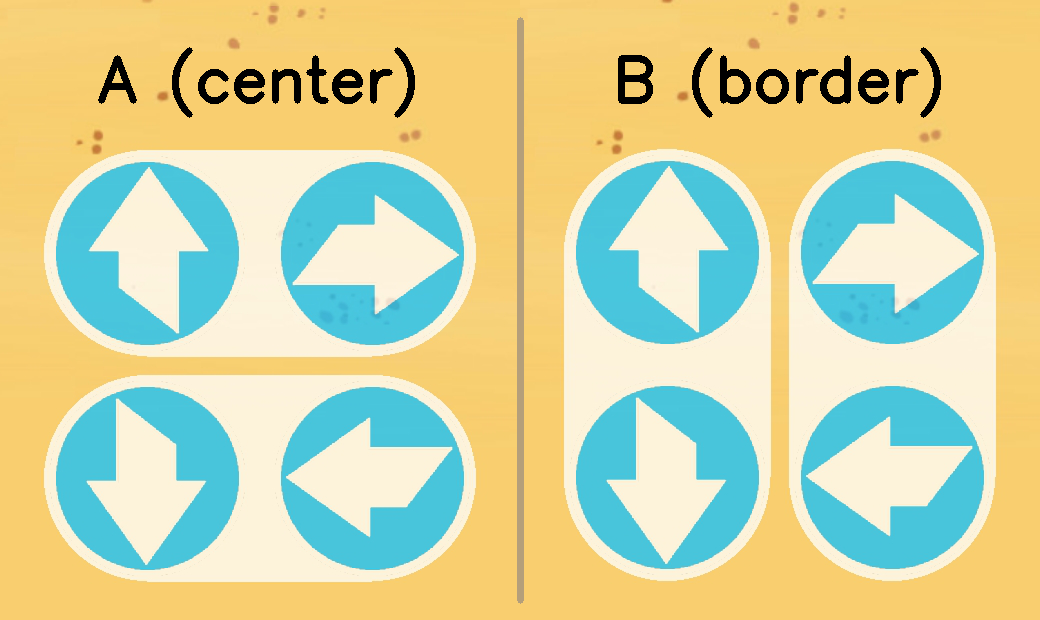
\includegraphics[width=1\linewidth]{controls} \\ (а)
    \end{minipage}
    \hfill
    \begin{minipage}[b][][b]{0.49\linewidth}\centering
        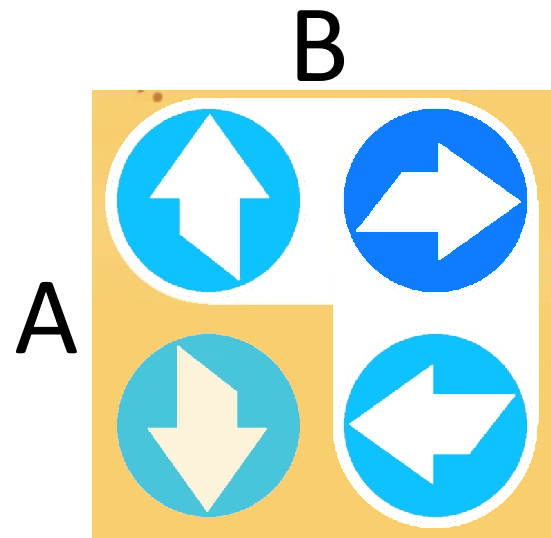
\includegraphics[width=0.73\linewidth]{fig1e} \\ (б)
    \end{minipage}
    \caption{
        (а) Кнопки управления для игрока А, целью которого является удержание фишки внутри поля как можно дольше (центр), и для игрока Б, целью которого является скорейшее достижение границы. (б) Пример определения выбора результирующего движения фишки: игрок А выбрал первую строку (кнопку), ограничив движение направлениями вверх и вправо, игрок Б выбрал второй столбец, ограничив направления вправо и влево. В результате таких выборов игроков направление, которое выбрали оба игрока, оказывается на пересечении соответствующих столбца и строки, что дает итоговое направление движения -- вправо.
    }
    \label{fig:controls}
\end{figure}


\begin{figure}[ht]
    \centerfloat{
        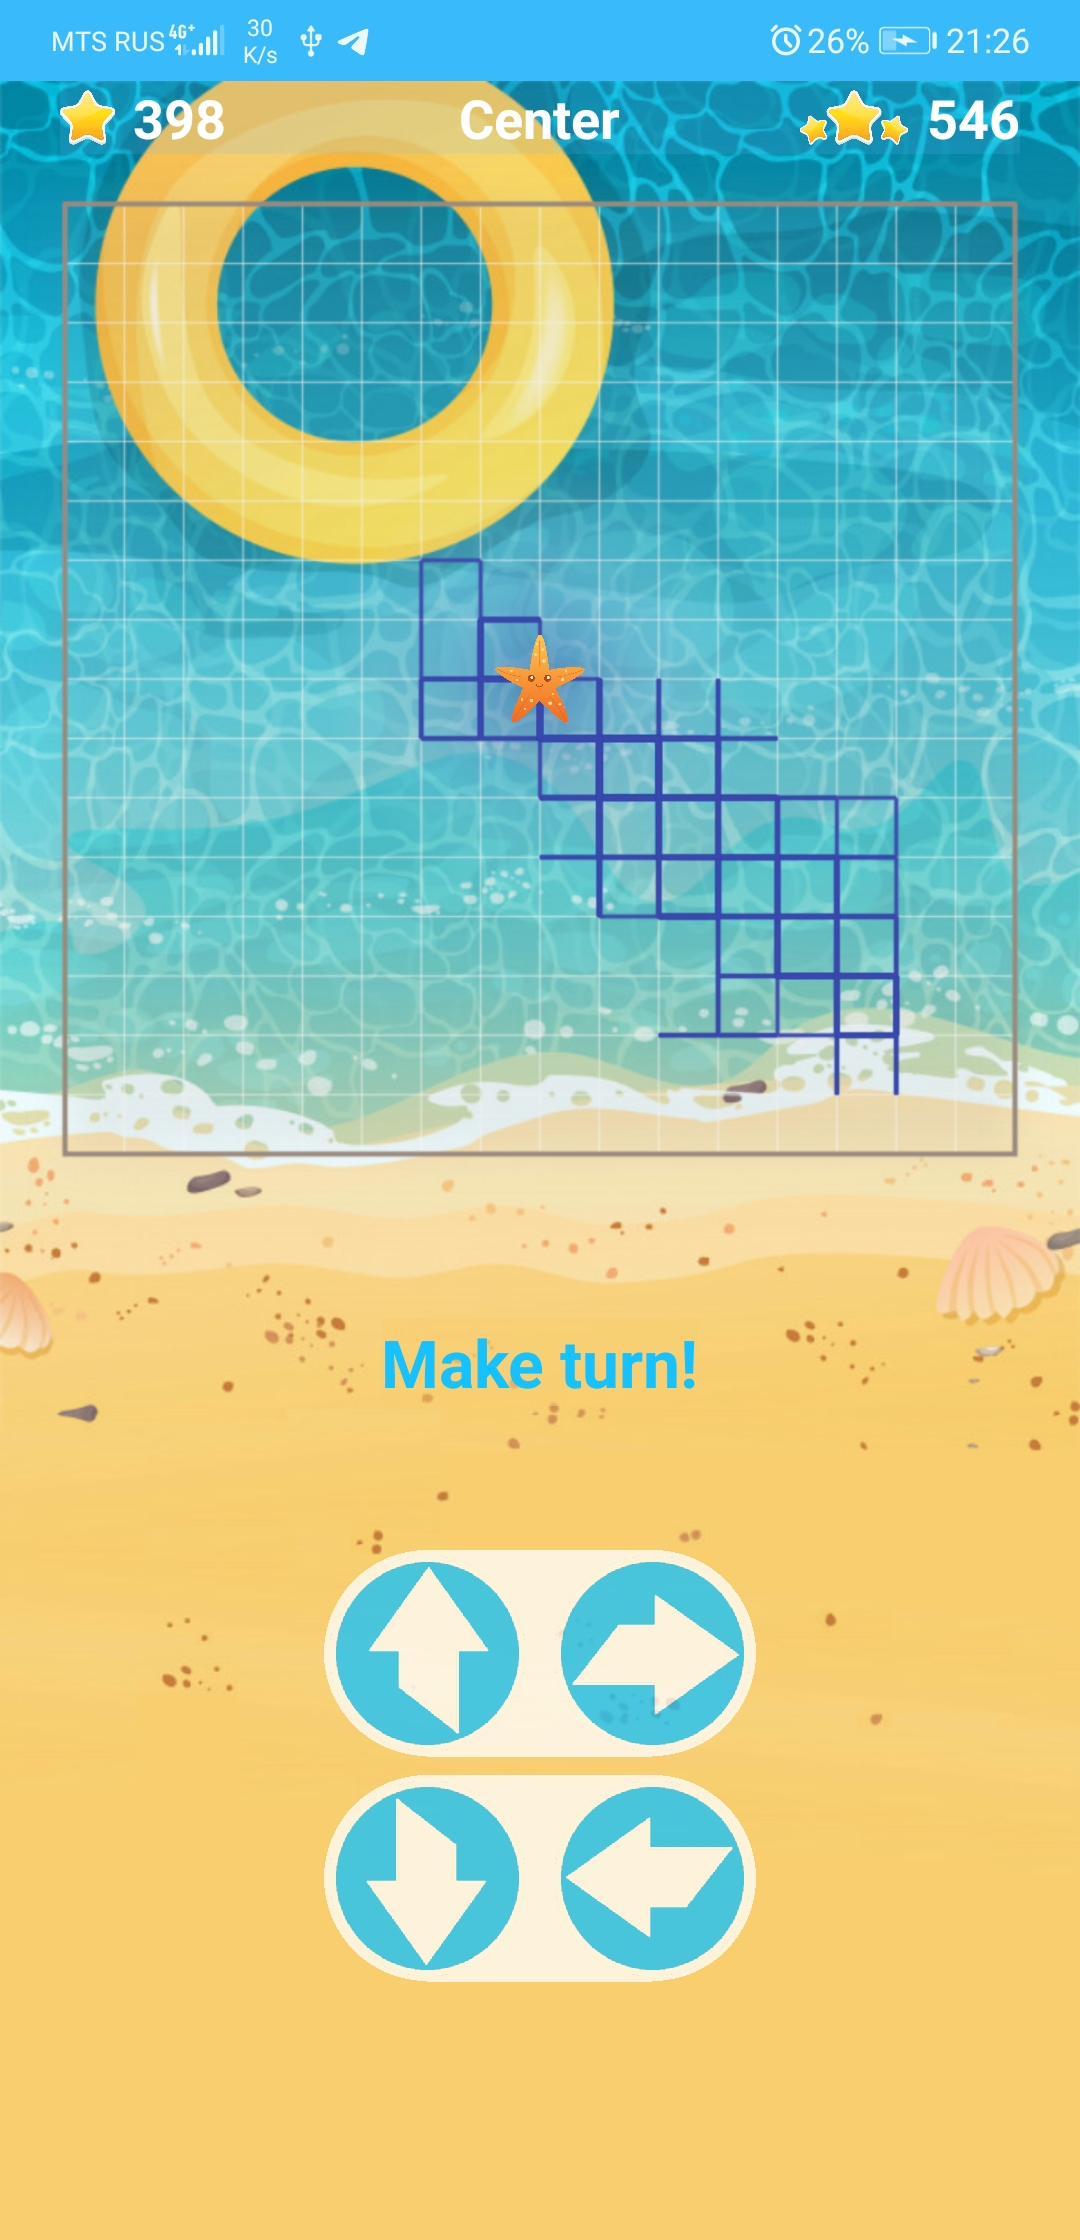
\includegraphics[scale=0.25]{screenshot_game_field}
    }
    \caption{
        Скриншот приложения Random Walk Game. Строка заголовка состоит из текущего количества ходов, целей игроков и количества ходов в самой длинной игре. Игрок видит игровое поле, положение фишки и траекторию фишки. Внизу экрана показана управляющая матрица $2$ на $2$, которая определяет результат совместного выбора стратегий игроками A и B. Строки представляют собой возможный выбор стратегий для игрока A, а столбцы -- для игрока B. Результирующее направление движения определяется стрелкой в ячейке, расположенной в соответствующих строке и столбце.
    }\label{fig:screenshot_game_field}
\end{figure}


Рассмотренные методы в предыдущей главе для численного моделирования процесса, моделирования эволюции вероятности и расчета фундаментальной матрицы были реализованы на языке Python 3.8. Применяя данные методы были вычислены статистические свойства и распределения, рассмотренные в разделе \cref{subsec:ch2/sec1/sub4} <<Моделирование эволюции вероятности>>, для сравнения с модельной и экспериментально полученной статистикой. Расчет трех подходов (численное моделирование, моделирование вероятностной эволюции, расчет фундаментальной матрицы) и их статистические свойства были выполнены на рабочей станции (Core i5-8600 3,1 ГГц, 32 ГБ ОЗУ). Исходный код программы обсчета доступен в репозитории на GitHub \cite{RWAnalyzer}.

Результаты рассматривают игру двух оппонентов на квадратной решетке для различных случаев: BvB -- случайное блуждание на квадратной решетке, PvP -- игра между двумя игроками, PvE игра за центр против компьютера, PvE игра за границу против компьютера. Сравнение с экспериментально полученными траекториями осуществлялось на поле $17 \times 17$ в играх с реальными игроками. Выбор размера поля был определен на основе наблюдений за игроками при игре на различных размерах поля. Анализ показал, что уменьшение размера поля приводит к быстрому завершению игры, что не дает игрокам находить качественные сложные стратегии. При увеличении размера поля игры длятся слишком долго, что вызывает усталость, снижение концентрации. Это в свою очередь ведет к уменьшению заинтересованности игрока, цель которого оставаться внутри поля, в длительном матче, а также к фрустрации игрока, цель которого достичь границы как можно скорее из-за многочисленных неудач. Вариант игры на поле $17 \times 17$ демонстрирует среднее время игры $10$-$15$ минут, что позволяет игрокам оставаться вовлеченными в процесс и придерживаться своих целей. Однако, длительные игры более часа также возникают в процессе проведения эксперимента. Дополнительный анализ таких игр также был проведен в рамках данной работы.

Суммарно, играя в Random Walk Game, участники эксперимента провели около $250$ часов для создания исследуемого набора траекторий. В результате было получено $1562$ траектории позиции фишки на поле и соответствующих выборов игроков для трех режимов игры. Дополнительно была собрана информация о времени совершения хода каждым из игроков. Далее проводится анализ статистических свойств полученных траекторий и стратегий игроков, а также их сравнение с результатами численного анализа, моделирования и аналитических расчетов.

\section{Методы исследования игровых случайных блужданий}\label{sec:ch3/sec2}

Предложенная игровая динамика предполагает наличие двух игроков, осуществляющих свой выбор на каждом ходу исходя из некоторой стратегии. Одним из вариантов стратегии игроков может выступать случайный равновероятный выбор одной из кнопок на каждом ходу. Применение такой стратегии обоими игроками сводит игру к чистому случайному блужданию на ограниченной решетке -- обозначим такой случай как BvB (Bot vs Bot). Второй вариант состоит в игре человека, применяющего произвольную стратегию, против стратегии равновероятного выбора независимо от состояния -- обозначим как PvE (Player vs Environment). В этом случае различаются две стороны игры в зависимости от цели: как можно скорее достичь границу (игра за границу) и как можно дольше оставаться внутри поля (игра за центр). Последний рассмотренный вариант состоит в игре двух игроков, выбирающих произвольные стратегии (PvP -- Player vs Player).

\nomenclature{BvB}{Bot vs Bot}
\nomenclature{PvE}{Player vs Environment}
\nomenclature{PvP}{Player vs Player}

\subsection{Поглощающие Марковские цепи}\label{subsec:ch3/sec2/sub1}

Основным математическим подходом к анализу игровой динамики была выбрана теория цепей Маркова \cite{gagniuc_markov_2017}. Цепь Маркова характеризует дискретный (во времени) случайный процесс, в котором вероятность наступления каждого события зависит только от состояния, достигнутого в предыдущем событии. Представим состояние цепи в игре вектором координат положения фишки на квадратной решетке $w_k = (x_k, y_k)$ на $k$-м ходе, при этом координаты находятся в пределах:
\begin{equation}
    -\lfloor n/2 \rfloor \leq x_k \leq \lfloor n/2 \rfloor, -\lfloor n/2 \rfloor \leq y_k \leq \lfloor n/2 \rfloor. 
    \label{eq:all-states}    
\end{equation} 
Всего в полученной цепи имеется $n^2-4$ достижимых узлов, $r=4(n-2)$ из которых соответствуют поглощающим (граничным) состояниям множества 
\begin{equation}
    \textbf{S}_{abs} = \{(x,y) : |x|=\lfloor n/2 \rfloor \lor |y|=\lfloor n/2 \rfloor\}
    \label{eq:border-states}
\end{equation}
и остальные $s=(n-2)^2$ -- переходным (внутренним) состояниям 
\begin{equation}
    \textbf{S}_{tr} = \{(x,y): |x|<\lfloor n/2 \rfloor \land |y|<\lfloor n/2 \rfloor\},
    \label{eq:inner-states}
\end{equation}
см. Рис.~\cref{fig:game_field}. 

Хотя существует 2 случая четности размера решетки, в работе рассмотрены только нечетные размеры, при которых начальное состояние расположено в центре поля и решетка обладает симметриями относительно центра. Минимально возможный размер такого игрового поля $3 \times 3$. 

Описание цепи в теории Марковских цепей представляется в виде матрицы переходов \cite{kemeny_finite_1976} $\mathsf{P}$ с элементами,
соответствующими вероятностям $P((i, j) \rightarrow (x, y))$ изменения состояния из $(i, j)$ в $(x, y)$.

\begin{figure}[ht]
    \centerfloat{
        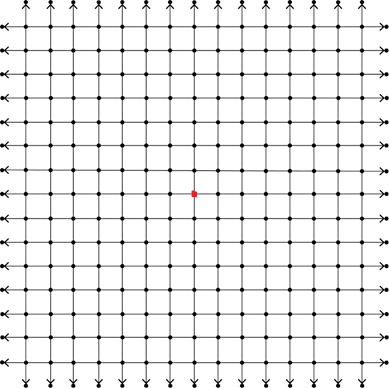
\includegraphics[width=0.5\linewidth]{game_field}
    }
    \caption{
        %Решетка игрового поля, состоящая из внутренних узлов (серые) и граничных узлов (красные), по достижении которых происходит завершение игры.
        Решетка игрового поля, состоящая из внутренних узлов и граничных узлов, по достижении которых происходит завершение игры.
        Стартовый узел отмечен в центре симметричного поля нечетного размера $17 \times 17$.
    }\label{fig:game_field}
\end{figure}

Теория поглощающих Марковских цепей предоставляет возможности для расчета статистики времен поглощения \cite{kemeny_finite_1976}. В теории поглощающих Марковских цепей матрица переходов $\mathsf{P}$ представляется в виде блочной матрицы:
\begin{equation}
    \begin{aligned}
    \mathsf{P}=
      \begin{bmatrix}
        Q & R \\
        \textbf{0} & I_r
      \end{bmatrix}
    \label{eq:P}
    \end{aligned}
\end{equation}
где $Q$ это матрица размера $s \times s$, характеризующая переходы между внутренними состояниями, 
$R$ -- ненулевая матрица размера $s \times r$, соответствующая переходам из внутренних состояний в поглощающие, $I_r$ -- единичная матрица размера $r \times r$, описывающая свойство петель в поглощающих состояниях, совместно с нулевой матрицей $\textbf{0}$ размера $r \times s$, указывающей на невозможность выхода из поглощающего состояния (поглощение) \cite{kemeny_finite_1976}.

Применяя многократно матрицу переходов для внутренних состояний и проводя суммирование результирующей матрицы по всем моментам времени, теория поглощающих Марковских цепей вводит понятие фундаментальной матрицы $N$. Так как матрица $Q$ имеет норму меньшую единицы и является сжимающим отображением, то соответствующий ряд сходится и имеет место следующая замкнутая форма вычисления фундаментальной матрицы:
\begin{equation}
    \begin{aligned}
    N=\sum_{k=0}^{\infty} Q^k=(I_s-Q)^{-1}
    \label{eq:N}
    \end{aligned}
\end{equation}
где $I_s$ это единичная матрица размера $s \times s$. Элемент фундаментальной матрицы $N$ с индексами $(i, j)$ является математическим ожиданием количества раз обнаружить цепь в состоянии $j$, при условии начала блуждания в состоянии $i$.

Используя свойство фундаментальной матрицы теория дает способ вычислить ожидаемое число шагов до поглощения при условии начала блуждания в некотором внутреннем состоянии $i$:
\begin{equation}
    \begin{aligned}
    T=N\textbf{1}
    \label{eq:T}
    \end{aligned}
\end{equation}
где $\textbf{1}$ вектор все элементы которого единицы.

В рассматриваемой игровой механике стартовая позиция игры находится в центре решетки. 
Тогда соответствующее математическое ожидание числа ходов до поглощения $\boldsymbol{\mathsf{t_n}}$ ($n$ -- размер поля) 
будет записано в элементе вектора $T$, соответствующем состоянию цепи с положением $(0, 0)$ на игровой решетке.

%\subsection{Игра в терминах цепи Маркова}\label{subsec:ch2/sec1/sub3}

Игровая механика Random Walk Game предполагает игру двух оппонентов, на каждом ходу определяющих свой выбор одного из двух доступных вариантов.
В общем случае, каждый из игроков обладает памятью и может ориентироваться на предысторию ходов оппонента.
Формулировка игры в виде Марковского процесса позволяет одному из игроков вычислить равновесие Нэша в смешанных стратегиях \cite{nash_non-cooperative_1951}.
Наличие такого равновесия и независимость стратегии от номера хода одного игрока не позволит другому игроку использовать предысторию ходов
для получения большего выигрыша в среднем. Таким образом при оптимальной игре обоих игроков процесс будет являться Марковским.

Рассмотрим подробнее математическую формулировку в терминах поглощающих Марковских цепей игры Random Walk Game.
Независимая от номера хода стратегия игрока $S_{ij}^p$ описывается распределением Бернулли $\sigma_{ij}^p$ для игрока 
$p \in \{A, B\}$ в состоянии с координатами $(i, j)$:

\begin{equation}
    \begin{aligned}
    \boldsymbol{\sigma}_{ij}^p(s)=
    \begin{cases}
        f_{ij}^p, &\mbox{if } s = 0,\\ 
        1-f_{ij}^p, &\mbox{if } s = 1,\\
    \end{cases}
    \label{eq:sigma}
    \end{aligned}
\end{equation}
где $0 \leq f_{ij}^p \leq 1$ -- вероятность выбора игроком первого варианта хода $(s=0)$.

Определение движения фишки на поле осуществляется после выбора обоими игроками своего варианта хода в соответствии с правилами,
описанными в разделе \cref{subsec:ch1/sec2/sub1} <<Описание игры>> и на Рис.~\cref{fig:controls}. 
Движение возможно в одном из 4 направлений в соседние состояния:
$(i, j + 1), (i + 1, j), (i, j - 1), (i - 1, j)$. Результирующее направление определяется совместным распределением, 
задающим вероятность перехода из состояния $(i, j)$ в состояние $(x, y)$:
\begin{equation}
    \begin{aligned}
    P& \left( (i, j) \rightarrow (x, y) \right) = \\
    &=\begin{cases}
        0, &\mbox{if } |i-x|+|j-y| \neq 1,\\ 
        f_{ij}^A \left(1-f_{ij}^B\right), &\mbox{if } x=i \land y=j+1, \boldsymbol{\rightarrow}\\
        \left(1-f_{ij}^A\right) f_{ij}^B, &\mbox{if } x=i+1 \land y=j, \boldsymbol{\downarrow}\\
        \left(1-f_{ij}^A\right) \left(1-f_{ij}^B\right), &\mbox{if } x=i \land y=j-1, \boldsymbol{\leftarrow}\\
        f_{ij}^A f_{ij}^B, &\mbox{if } x=i-1 \land y=j, \boldsymbol{\uparrow}\\
    \end{cases}
    \label{eq:transition}
    \end{aligned}
\end{equation}

Первый случай в формуле определяет нулевую вероятность перехода между несвязанными состояниями, и оставшиеся соответствуют четырем направлениям движения фишки.

Наборы значений $f_{ij}^p$ для двух игроков $(p \in \{A, B\})$ задают их стратегии в каждом узле квадратной решетки $(i, j)$. 
Фиксация этих значений до начала игры позволяет вычислить матрицу вероятностей переходов между состояниями, то есть полностью определить Марковскую цепь.
Наиболее общий случай игры PvP позволяет обоим игрокам задавать свой набор вероятностей $f_{ij}^p$. В случае игры против среды PvE
стратегия одного из игроков известна и представляет собой равновероятный выбор среди двух возможных вариантов независимо от позиции на поле и номера хода: $f_{ij}^{p_1} = 0.5, (p_1 \in \{A, B\})$, а для второго игрока значения определяются произвольно $f_{ij}^{p_2}, (p_2 \in \{A, B\} \setminus \{p_1\})$. 
Вырожденный случай игры BvB случайного блуждания определяется равновероятным выбором обоих игроков одного из вариантов хода $f_{ij}^{A} = f_{ij}^{B} = 0.5$
для всех состояний игры. В этом случае вероятность перехода из каждого внутреннего состояния в соседнее равно $\frac{1}{4}$.

Оба игрока рассматривают в качестве цели количество ходов в игре. Цель одного минимизировать количество ходов, а цель второго -- максимизировать.
В случае Марковской цепи при определенных смешанных стратегиях игроков целевой функцией является математическое ожидание времени достижения границы.
Обозначим соответствующие средние времена поглощения в игре для 4 случаев как $\boldsymbol{\mathsf{t_n^{BvB}}}$, 
$\boldsymbol{\mathsf{t_n^{PvEA}}}$, $\boldsymbol{\mathsf{t_n^{PvEB}}}$ и $\boldsymbol{\mathsf{t_n^{PvP}}}$.

\subsection{Моделирование эволюции вероятности}\label{subsec:ch2/sec1/sub4}

Аналитический подход теории поглощающих Марковских цепей позволяет вычислить значение среднего времени поглощения случайного блуждания
с применением матричных преобразований. Однако теории для расчета точного распределения времени поглощения в случае Марковских цепей
разработано не было. Прямой подход к расчету оценки распределения времени поглощения возможен благодаря математическому моделированию процесса 
эволюции вероятности. Дополнительным преимуществом данного подхода является возможность оценки наряду с распределением времени достижения также 
пространственного распределения вероятностей. 

Рассмотрим подробнее модель эволюции вероятности. Пусть $W_{ij}^{k}$ -- вероятность найти фишку в состоянии $(i, j)$ в момент времени $k$. Начальное состояние игры в центре поля $(0, 0)$ соответствует единичной вероятности найти частицу в начальный момент времени $t=0$ в состоянии $(0, 0)$, то есть $W_{0,0}^{0}=1$ и $W_{ij}^{0}=0$ для остальных состояний $((i, j) \neq (0, 0))$. Упорядочим все состояния последовательно по формуле $in + j$, где $n$ -- размер поля. Тогда вектор $\boldsymbol{w^{0}}$ описывает распределение вероятности в начальный момент времени, а для всех моментов времени $k > 0$ распределения последовательно определяются по формуле эволюции вероятности:
\begin{equation}
    \begin{aligned}
    \boldsymbol{w^{k+1}}=\mathsf{\widetilde{P}}\boldsymbol{w^{k}}, k \geq 0
    \label{eq:evolution}
    \end{aligned}
\end{equation}
где $\mathsf{\widetilde{P}}$ -- модифицированная матрица вероятностей переходов между состояниями цепи. 

Эволюция вектора вероятности на каждом шаге также дает возможность оценить точную вероятность $W_{ij}^{k}, (i, j) \in \boldsymbol{B}$ окончания блуждания на $k$-ом ходу в граничном состоянии $(i, j)$. Для этого используется модифицированная матрица переходов такая, что при достижении границы фишкой происходит ее исключение из системы. Тогда вероятность поглощения частицы на $k$-ом шаге может быть вычислена по следующей формуле:

\begin{equation}
    \begin{aligned}
    p_\mathsf{abs}^{k}=\sum_{(i, j) \in \boldsymbol{\mathsf{B}}} W_{ij}^{k},
    \label{eq:timedistr}
    \end{aligned}
\end{equation}
где $\textbf{B}$ -- множество граничных состояний.

Моделирование эволюции вероятности также позволяет вычислить пространственное распределение вдоль граничных состояний за счет аппроксимации ряда вероятностей поглощения в узле $(i, j) \in \boldsymbol{\mathsf{B}}$ по всем моментам времени:
\begin{equation}
    \begin{aligned}
    p_{ij}^\mathsf{abs}=\sum_{k=0}^{\infty} W_{ij}^{k}
    \label{eq:spacedistr}
    \end{aligned}
\end{equation}

В связи с экспоненциальным убыванием вероятности $W_{ij}^{k}$ с ростом номера $k$ суммирование выполняется до достижения заданной точности модуля разности между соседними членами.

Дополнительным свойством, представляющем интерес при анализе игровой динамики, является соотношение вероятностей закончить игру на четном числе ходов или на нечетном. Отличие этого соотношения от единицы обусловлено тем, что квадратная решетка представляет собой двудольный граф, в связи с чем на каждом ходу фишка может находится только в одной из долей в зависимости от четности хода. Обозначим долю графа четной, если фишка находится в ней на четном ходу, и нечетной -- если на нечетном ходу. Состояния $(i, j)$ двух долей расположены на решетке в шахматном порядке и аналогично могут быть отнесены к "четным" и "нечетным" состояниям в соответствии с четностью суммы координат $(i + j) \mod 2$. Распространение вероятности по цепи происходит за счет полного перехода между долями. Однако вероятность поглощения в четных и нечетных состояниях отличается ввиду разного количества и расположения поглощающих состояний в долях.

Применение подхода к моделированию эволюции вероятности позволяет численно получить большой спектр информации о свойствах игры.

%\subsection{Численное моделирование}\label{subsec:ch2/sec1/sub5}

Анализ статистических свойств игровой динамики возможен благодаря подходам, использующим теорию Марковских цепей и моделирование эволюции вероятности. Однако исследование структурных особенностей индивидуальных траекторий требует применения методов численного моделирования. Одним из способов решения задачи является метод Монте-Карло для симуляции случайного процесса с использованием генератора случайных чисел. Сталкивая различные смешанные стратегии, исследуемые в ходе работы, возможно построить последовательность перемещений фишки по решетке, движущейся в соответствии с правилами игры. Алгоритм симуляции состоит из нескольких шагов:
\begin{itemize}
\item Начальное положение фишки определяется в центре поля $(0, 0)$. 
\item На каждом ходе генерируются выборы игроков из распределения с соответствующей стратегией игрока с использованием псевдослучайного генератора Mersenne Twister \cite{matsumoto_mersenne_1998} из модуля random в Python 3.8.
\item В соответствие с правилами перехода фишка перемещается в одно из соседних состояний.
\item По достижении фишкой одного из граничных состояний симуляция останавливается.
\end{itemize}

В результате работы алгоритма генерируется последовательность ходов игроков и движений фишки на поле. Для визуализации индивидуальных траекторий реализованы три способа: 
\begin{itemize}
\item визуализация всех ходов траектории с наложением на одной плоскости;
\item разбиение ходов на последовательные группы по 40 ходов и визуализация групп блоками от первой до очередной группы;
\item анимация движения фишки и след траектории с затуханием.
\end{itemize}

Дополнительно, при сравнении с результатами моделирования эволюции вероятности были вычислены частоты встречаемости времен полученных игр. 

\subsection{Полевой эксперимент с применением мобильных приложений и сети интернет}\label{subsec:ch2/sec2}

Математический подход к анализу стратегий дает возможность выявить наиболее оптимальные способы действия игроков. Однако в реальных условиях на поведение человека, принимающего решение о конкретном ходе, влияет большой спектр факторов: настроение, предыдущие действия игроков, внешние обстоятельства и т.д. Естественный подход к продолжению анализа игровой динамики состоит в проведении полевого эксперимента с участием людей в качестве игроков. 

Для участия в эксперименте были приглашены волонтеры в возрасте от 16 до 52 лет. Игроки до 25 лет были отобраны из числа студентов ННГУ им. Н.~И.~Лобачевского и Высшей школы экономики. Игроки старше 25 лет были набраны из разных университетов и исследовательских институтов России, Германии, Норвегии и Южной Кореи.

Основной критерий для отбора участников состоял в основном роде деятельности заключающемся в умственном труде. Большая часть участников представляет собой успешных студентов, призеров олимпиад, профессоров, кандидатов наук, успешных ИТ-специалистов.

Проведение эксперимента состояло из четырех отдельных мероприятий:
\begin{itemize}
\item Организованные игры без конкурса между участниками. Студенты находились в одной комнате и играли не общаясь друг с другом в течение одного часа. Интерес участников заключался в достижении самой длинной игры среди участников. Пары игроков выбирались на основе схожести их навыков в олимпиадном программировании.
\item Конкурс на получение наибольшего количества очков при игре против среды PvE. Участники играли онлайн в течение месяца соревнуясь с другими участниками в общем рейтинге. Рейтинг представлял собой отношение двух экспоненциально скользящих средних длительностей по играм за центр и за границу. Общий рейтинг все время был доступен участникам.
\item Личный чемпионат между студентами в играх PvP. Студенты находились в одной аудитории и играли не общаясь друг с другом в течение двух часов. Участники распределялись по взвешенной сумме длин сыгранных игр. Чем длиннее игра -- тем выше вес, связанный с этой игрой для участника, играющего за центр (A) и противоположный для участника, играющего за границу (B). Интерес участников заключался в получении наивысшего места в таблице.
\item Свободные игры без конкурса между участниками и между участником и средой. Участники находились дома и играли не общаясь около 30 минут в день. Интерес участников состоял в получении наибольшего (наименьшего) счета в конкретной игре. В любой момент игроки могли приостановить игру и продолжить ее в удобное для них время.
\end{itemize}

Цели игроков распределялись между ними равновероятно на основе генератора случайных чисел. В результате реализации эксперимента было собрано 500 игр типа PvP, 500 игр типа PvE за центр и 500 игр типа PvE за границу.

Для организации экспериментальной части было разработано мобильное приложение, доступное в Google Play Store \cite{googleplay} и в App Store \cite{applestore}. Приложение предоставляет два режима игры: игра против другого игрока (PvP) или игра против среды (PvE). В обоих режимах приложение отправляет выбор игроков через Интернет на веб-сервер и рассчитывает направление и следующую позицию фишки на поле. Результаты игр (траектории и соответствующие выборы стратегий игроков на каждом ходу) были собраны в базе данных на сервере для дальнейшего анализа. Основной экран мобильного приложения с игровым полем представлен на Рис.~\cref{fig:screenshot_game_field}.

Выбор одной из двух стратегий среды в режиме PvE определяется последовательностью псевдослучайных чисел, вычисленных генератором случайных чисел Mersenne Twister (реализованным в PHP 7.4 как функция $\mathsf{mt\_rand}$) \cite{matsumoto_mersenne_1998}. Игры, полученные в эксперименте, проводились на поле размера $17 \times 17$.

Архитектура системы состоит из трех основных компонент: мобильное приложение, веб-сервер и база данных. Взаимодействие между мобильным приложением и веб-сервером осуществляется посредством REST API по защищенному протоколу HTTPS через сеть Интернет. Процесс взаимодействия клиента и сервера состоит из нескольких этапов:
\begin{itemize}
\item Пользователь осуществляет регистрацию в системе, информация о регистрации отправляется на веб-сервер и сохраняется в базу данных (БД).
\item Пользователь аутентифицируется в системе на основе связки логин и пароль, либо на основе OAuth аутентификации.
\item Успешная аутентификация авторизует пользователя в системе и предоставляет список текущих игр пользователя, историю игр пользователя, рейтинг участников, и возможность начать новую игру.
\item Игрок инициирует игру с другим игроком по логину, случайным образом или выбором незавершенной игры из списка.
\item После инициализации двумя игроками одной и той же игры, выбранная каждым игроком стратегия на ходе передается на веб-сервер и сохраняется в БД.
\item Клиент опрашивает веб-сервер до тех пор, пока оба игрока не совершат выбор в текущем ходе.
\item После совершения выбора обоими игроками веб-сервер определяет направление движения фишки, факт достижения границы и по запросу передает на клиент эту информацию.
\item На клиенте обновляется положение фишки, количество ходов. Игра переходит на следующий ход или завершается.
\end{itemize}

\nomenclature{REST API}{Representational state transfer Application Programming Interface}
\nomenclature{БД}{База данных}

В качестве HTTP-сервера используется веб-сервер nginx \cite{reese_nginx_2008}. Программная часть, реализующая функционал серверной части, разработана на языке PHP 7.4 \cite{Nixon_web_2016} без использования дополнительных фреймворков с использованием модели Model-View-Controller (MVC) \cite{pitt_pro_2021}. Хранение информации реализовано на основе реляционной базы данных MySQL с применением хранимых процедур для защиты от XSS атак к базе данных \cite{stuttard_web_2011}.Защита паролей осуществляется с применением хеширования с солью на основе алгоритма bcrypt (реализовано в PHP 7.4 как функция $\mathsf{password\_hash}$).

\nomenclature{XSS}{Cross Site Scripting}
\nomenclature{MVC}{Model-View-Controller}

Мобильное приложение разработано с применением технологии Xamarin на языке C$\mathsf{\#}$ \cite{sole_xamarin_2022}. Преимуществом данной технологии в сравнении с другими, такими как Kotlin в среде разработки Android Studio, Objective-C, Swift в среде разработки XCode, является кроссплатформенность при сохранении общей кодовой базы бизнес-логики и возможности индивидуализации интерфейса пользователя по конкретную платформу. Xamarin предлагает три платформы для сборки приложения: Universal Windows App, Android, iOS. Наличие широкого выбора компонент, оптимизированных для разных платформ, позволило в короткие сроки разработать мобильное приложение для трех платформ. Основным паттерном проектирования приложения был выбран подход Model-View-ViewModel (MVVM). Разделение приложения на логически связанные компоненты и построение качественной архитектуры позволило сделать приложение гибким к внесению дополнительных изменений.

\nomenclature{MVVM}{Model-View-ViewModel}

\section{Численный анализ игры}\label{sec:ch3/sec3}

Основной целью для игроков является увеличение или уменьшение количества ходов, за которое будет достигнута граница поля.
Однако, основная особенность рассматриваемой игры состоит в наличии случайной компоненты, не зависящей напрямую от игроков и лежащей в основе механики их взаимодействия.
Для исключения влияния случайной компоненты на результирующий функционал был предложен подход к оценке среднего количества ходов,
за которое фишка достигнет границу поля (среднее время игры).
Применение такого подхода позволяет находить оптимальные стратегии, дающие максимум или минимум среднего времени игры в зависимости от цели игрока.

% \subsection{Вырожденный случай BvB неуправляемого случайного блуждания}\label{subsec:ch3/sec1/sub1}

% В случае BvB игроки совершают равновероятный выбор на каждом ходу одного из двух выборов, то есть среднее время игры зависит только от размера поля.
% Применяя метод расчета фундаментальной матрицы для поглощающей Марковской цепи для разных размеров поля были получены значения среднего времени игры для случая BvB.
% Используя аппроксимацию квадратичной зависимостью на основе метода наименьших квадратов (МНК) зависимости среднего времени для размеров полей в диапазоне от $3$ до $1001$
% были получены численные коэффициенты параболы: $\boldsymbol{\mathsf{t_n^{BvB}}} = 0.294685413 n^2 - 0.232$ (Рис.~\cref{fig:quadratic:time}). Средняя абсолютная ошибка аппроксимации составила $10^{-3}$. 
% Хотя простого способа представления в замкнутой форме данной зависимости еще не было найдено, в работе \cite{kmet_gamblers_2002} была предложена форма из нескольких сумм, позволяющая оценить
% среднее время игры для случая BvB, как простого случая случайного блуждания на ограниченном квадрате.

% \subsection{Задача глобальной оптимизации для случая PvE}\label{subsec:ch3/sec1/sub2}

% Рассмотрение случаев PvE приводит к необходимости поиска оптимальных стратегий. В связи с этим возникает постановка задачи 
% математического программирования по глобальной оптимизации среднего времени игры в пространстве стратегий. 
% Как было рассмотрено в разделе \cref{subsec:ch2/sec1/sub3} <<Игра в терминах цепи Маркова>> в соответствии с формулой \eqref{eq:transition} функция среднего времени игры
% зависит от двух векторов с вещественными элементами из диапазона $[0, 1]$, характеризующих стратегии каждого из игроков.
% В случае PvE стратегия одного из игроков фиксирована и может быть исключена из аргументов задачи оптимизации.
% Тогда возникают две независимые задачи оптимизации для случаев игры за центр и за границу:
% \begin{equation}
%     \begin{aligned}
%         \boldsymbol{\mathsf{t_n^{PvEA}}} = \max_{f^A \in \boldsymbol{\mathsf{F}}} \boldsymbol{\mathsf{t_n}}, \hspace{1em} f_{ij}^B=1/2,
%     \label{eq:centeropt}
%     \end{aligned}
% \end{equation}
% \begin{equation}
%     \begin{aligned}
%         \boldsymbol{\mathsf{t_n^{PvEB}}} = \min_{f^B \in \boldsymbol{\mathsf{F}}} \boldsymbol{\mathsf{t_n}}, \hspace{1em}  f_{ij}^A=1/2,
%     \label{eq:borderopt}
%     \end{aligned}
% \end{equation}
% где $\boldsymbol{\mathsf{F}}$ -- пространство векторов с элементами в диапазоне $[0, 1]$, которые соответствуют выбранным относительным частотам $f_{ij}^p$
% в смешанных стратегии игрока $p \in [A, B]$. Расчет $\boldsymbol{\mathsf{t_n}}$ осуществляется с применением рассмотренного подхода поглощающих Марковских цепей
% в разделе \cref{subsec:ch2/sec1/sub2} <<Поглощающие Марковские цепи>> с использованием формул \eqref{eq:P}, \eqref{eq:N}, \eqref{eq:T}, \eqref{eq:transition}.

% Количество переменных в задаче оптимизации растет квадратично с ростом размера поля, что существенно усложняет анализ для выбранных размеров $17 \times 17$.
% Однако для случаев с небольшим числом оптимизируемых переменных задача может быть решена напрямую поиском глобального оптимума.
% Применяя алгоритм \texttt{Minimize} математического пакета Wolfram Mathematica для решетки размеров $5$ и $7$ удалось получить значения
% оптимального времени игры для случаев игры против случайного равновероятного выбора компьютером (PvE), а также набор найденных стратегий.
% Случай $3 \times 3$ не представляет прямого интереса, так как среднее время поглощения равно $1$ независимо от выбора стратегий игроков, 
% так как поглощение фишки происходит на первом ходу. Случай $5 \times 5$ уже не является вырожденным и выборы игроков влияют на результат среднего времени игры.
% Всего при решении данного случая возникает задача оптимизации с $9$ параметрами, которая может быть решена с применением \texttt{Minimize}.

% Количество параметров для решения задачи большего размера при использовании данного подхода слишком велико, что не позволяет без упрощения найти оптимальную стратегию.
% Для уменьшения размерности воспользуемся симметриями в игре стратегий игроков относительно главной и побочной диагоналей. 
% Две симметрии позволяют свернуть игру уже на одном из $4$ треугольников между главной и побочной диагоналями. 
% Для определенности выберем верхний треугольник. Тогда верхняя граница, как и ранее, соответствует граничным поглощающим состояниям,
% а две новые стороны треугольника соответствуют отражающим границам, то есть из состояний на диагонали возможно перейти только в $2$ соседних состояния внутри треугольника.
% Учет данных симметрий позволяет приблизительно в $4$ раза уменьшить количество состояний и соответственно количество различных элементов в векторе стратегий,
% что позволило решить задачу для случая $7 \times 7$. 

% \subsection{Гипотеза об оптимальных стратегиях для случая PvE}\label{subsec:ch3/sec1/sub3}

% Анализируя стратегии и значения среднего времени игры, найденные с применением глобальной оптимизации, для малых размерностей,
% а также учитывая свойства игры, для достижения оптимальных значений были предложены $2$ стратегии \cite{confbib1}.
% Случай PvE состоит из двух вариантов игры: с целью удержать фишку как можно дольше внутри поля (максимизировать среднее время игры)
% и с целью как можно скорее достичь границы (минимизировать среднее время игры). 
% Значения оптимального среднего времени игры для обоих случаев представляют квадраты нечетных чисел для малых размеров поля.
% В случае PvE при игре за центр формула представляется в виде: $\boldsymbol{\mathsf{t_n^{PvE A}}} = (n-2)^2$ и в случае
% игры за границу в виде: $\boldsymbol{\mathsf{t_n^{PvE B}}} = \frac{(n-1)^2}{4}$. 

% В предположении сохранения такой же закономерности для больших размеров поля, рассмотрим стратегии, достигающие
% средних времен игры $\boldsymbol{\mathsf{t_n^{PvE B}}}$ и $\boldsymbol{\mathsf{t_n^{PvE A}}}$. Принцип построения стратегии в обоих случаях 
% состоит в выборе некоторой одномерной структуры внутри поля, на которой игрок может поддерживать блуждание без выхода за границу этой структуры.
% Такая структура будет представлять собой одномерную марковскую цепь, по которой игрок может осуществлять некоторое блуждание.
% При этом большее количество узлов цепи будет соответствовать большим средним временам. Таким образом в случае игры за центр
% необходимо выбрать наиболее длинную такую структуру, а в случае игры за границу наиболее короткую.

% Самая длинная одномерная цепь, внутри которой игрок за центр может сохранять свою фишку независимо от выборов второго игрока, 
% представляет собой <<лестницу>> состояний на главной диагонали. С характеристикой наиболее длинной цепи также существует побочная диагональ, однако
% правила игры не позволяют поддерживать случайное блуждание на ней независимо от ходов второго игрока. 
% Для поддержания фишки на <<лестнице>> главной диагонали игрок чередует свой выбор кнопок на каждом ходу.
% Выбор такой структуры позволяет получить одномерную марковскую 
% цепь длины $2n-3$, случайное блуждание вдоль которой осуществляется равновероятно в обоих направлениях, так как $f_{ij}^B=\frac{1}{2}$.
% Такая Марковская цепь соответствует случаю игры о разорении игрока с одной валютой. Применяя формулу для среднего времени случайного блуждания на отрезке \eqref{eq:eq6},
% рассмотренную в разделе \cref{subsec:ch1/sec1/sub1} <<Задача о разорении игрока>>, получим среднее время $\boldsymbol{t_n^{PvE A}} = ((2n-3-1)/2)^2 = (n-2)^2$ соответствующее обнаруженной закономерности.
% График зависимости представлен на Рис.~\cref{fig:quadratic:time}.

% Аналогично, применяя принцип поиска структуры одномерной цепи, выберем самую короткую цепь для случая игры за границу.
% Такой цепью будет являться горизонтальный или вертикальный отрезок, проходящий через центральную стартовую позицию.
% Независимо от выборов первого игрока, второй игрок сможет выбирая одну и ту же кнопку оставаться на данном отрезке.
% Полученная цепь состоит из $n$ состояний, что дает среднее время поглощения $\boldsymbol{\mathsf{t_n^{PvE B}}} = \frac{(n-1)^2}{4}$, 
% график зависимости представлен на Рис.~\cref{fig:quadratic:time}.
% Игрок не обязательно должен выбрать только один из отрезков, а может использовать их комбинацию, переходя в центральном узле между ними,
% ввиду симметрий рассмотренных в предыдущем разделе. 

% Рассмотренные стратегии не являются единственными достигающими найденные значения среднего времени игры. 
% Одна из стратегий для случая игры за центр, использующая не только одномерный набор состояний, а все игровое поле целиком, 
% может быть сформулирована следующим образом: в состояниях соседних с граничными выбор стратегии состоит в движении от границы или вдоль нее, 
% а во всех остальных состояниях выбор осуществляется произвольным образом. Применяя символьные вычисления Wolfram Mathematica
% в методе расчета среднего времени игры с использованием фундаментальной матрицы было продемонстрировано для размеров поля
% $5, 7, 9, 11$, что все переменные $f_{ij}^A$, соответствующие состояниям не инцидентным границе, после упрощения выражения имеют нулевые коэффициенты.
% Времена, получаемые при данной стратегии, также совпадают с найденной закономерностью $\boldsymbol{\mathsf{t_n^{PvE A}}}$.

% Все 3 найденных зависимости среднего времени игры для трех случаев представляют собой квадратичную функцию с различными коэффициентами
% (Рис.~\cref{fig:quadratic:time}).
% Старший коэффициент при $n^2$ для случая PvE за центр -- $1$, для случая PvE за границу -- $0.25$, для случайного блуждания BvB -- $0.29$.
% Таким образом, предполагаемая оптимальная стратегия в случае PvE игры за центр показывает время в $3.4$ раза большее, чем случайный равновероятный выбор игрока в случае BvB.
% В случае же игры PvE за границу время оказывается меньше, чем при случайном равновероятном выборе в случае BvB, приблизительно на $15\%$.

% \begin{figure}[t]
%     \centering
%     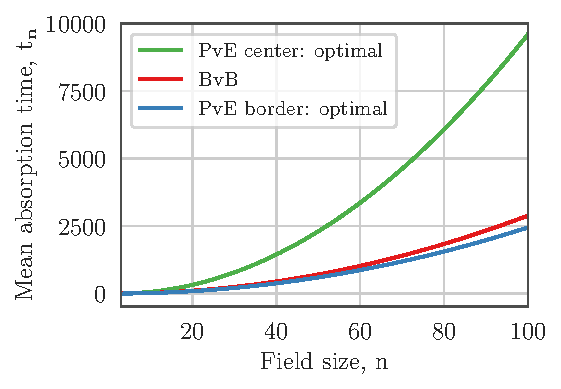
\includegraphics[width=\columnwidth,keepaspectratio,clip]{fig2.pdf}
%     \caption{
%         Квадратичные зависимости среднего времени поглощения от размеров поля для случаев: центр PvE для игрока A 
%         (цель игрока оставаться внутри как можно дольше) -- зеленая линия, 
%         граница PvE для игрока B (цель игрока достичь границу как можно скорее) -- синяя линия, 
%         BvB (времена поглощения чистого случайного блуждания) -- красная линия.
%     }  
%     \label{fig:quadratic:time}
    
% \end{figure}


% \subsection{Сравнение с экспериментальными результатами}\label{subsec:ch3/sec1/sub4}

% Следующим шагом в анализе игровой динамики является рассмотрение сравнения результатов моделирования с результатами 
% собранных игр в полевом эксперименте. Сбор траекторий в эксперименте осуществлялся с применением разработанной игры Random Walk Game
% и участием нескольких десятков людей. Подробное описание эксперимента приведено в разделе \cref{subsec:ch2/sec2} <<Полевой эксперимент>>. Суммарно в режиме 
% PvE было собрано $1062$ игры: $528$ -- игры за центр, $534$ -- игры за границу. 

% Участники, цель которых была удерживать фишку как можно
% дольше внутри поля в среднем показали $145.45$ ходов за игру. Сравнивая этот результат с предположительно оптимальной стратегией 
% среднее время которой равно $\boldsymbol{\mathsf{t_{17}^{PvE A}}} = (17-2)^2 = 225$, получаем отставание на $54\%$ реальных игр от результатов моделирования.
% Хотя игроки показали не оптимальное время игры, выбранная ими стратегия позволяет улучшить в $2$ раза результат относительно $75.2$ хода
% в случае равновероятного выбора (BvB). Эксперимент показал, что рассматриваемая группа игроков способна распознать свойства игры 
% и значительно улучшить среднее время игры несмотря на отсутствие априорного знания об оптимальной стратегии. 
% В качестве подтверждения качества стратегии, найденной игроками, были получены относительные частоты для каждой позиции на поле
% и проведено моделирование столкновения стратегий случайного выбора против стратегии игроков. В результате моделирования было получено 
% характерное среднее время игры $145.85$ согласующееся со средним временем экспериментальных траекторий.

% Результаты игр участников в случае PvE с целью скорейшего достижения границы продемонстрировали среднее количество ходов равное $71.12$.
% В сравнении с предполагаемой оптимальной стратегией, среднее время которой равно $\boldsymbol{\mathsf{t_n^{PvE B}}} = \frac{(17-1)^2}{4} = 64$, игроки 
% отстают на 7 ходов. Несмотря на такое отставание, среднее время игры у участников меньше на 4 хода, чем в случае равновероятного выбора. 
% Аналогично предыдущему случаю игры за центр, игроки показали улучшение относительно случайного блуждания BvB и достаточно большой разрыв со средним временем игры
% для предполагаемой оптимальной стратегии. Моделирование игровой динамики за счет столкновения стратегий равновероятного случайного выбора и 
% частот выборов, полученных из эксперимента, продемонстрировало отличие среднего времени игры, равного $73.79$, относительно среднего числа ходов в траекториях игроков.
% Предположительно, данное отличие вызвано неточными частотами в редко посещаемых состояниях. 

% Результаты эксперимента корректно воспроизводятся при использовании частот из экспериментальных игр для случая PvE в
% качестве входных вероятностей для процесса моделирования с применением эволюции вероятности и численного моделирования отдельных траекторий. 
% Таким образом, частоты выбора соответствующих стратегий, определенные для каждого состояния, позволили нам интерпретировать множество $f_{ij}$ как усредненную стратегию, 
% найденную группой участников эксперимента. Значения среднего времени игры представлены в сводной таблице (см. Таблицу~\cref{tab:time}).

% \begin{table}[]
%     %\setlength\extrarowheight{3pt}
%     \fontsize{10pt}{10pt}\selectfont
%     \begin{tabular}{|l|c|c|c|c|c|}%{|p{1.7cm}|C{1.2cm}|C{1.2cm}|C{1.2cm}|C{1.2cm}|C{1.2cm}|}
        
%         \toprule
%         %\multicolumn{1}{|c|}{\begin{tabular}[c]{@{}c@{}}Размер поля\\$17 \times 17$\end{tabular}} & \textbf{\begin{tabular}[c]{@{}c@{}}Random\\walk\end{tabular}} & \textbf{\begin{tabular}[c]{@{}c@{}}PvE центр\end{tabular}} & \textbf{\begin{tabular}[c]{@{}c@{}}PvE граница\end{tabular}} & \textbf{PvP} & \textbf{\begin{tabular}[c]{@{}c@{}}PvP\\ 400+\end{tabular}} \\ \hline
%         Размер поля $17 \times 17$ & \textbf{BvB} & \textbf{PvE центр} & \textbf{PvE граница} & \textbf{PvP} & \textbf{PvP $400+$} \\ 
%         \midrule
%         \textbf{Количество игр} & -     & 528    & 534   & 500    & 13     \\ 
%         %\specialrule{.1em}{.0em}{.0em}
%         \midrule
%         \textbf{Эксперимент}  & -     & 145.45 & 71.12 & 120.60 & 594.27 \\ 
%         \textbf{Моделирование траекторий}  & 75.22 & 145.77 & 73.66 & 115.93 & 132.91 \\
%         \textbf{Теория Марковских цепей}  & 75.21 & 145.85 & 73.79 & 116.22 & 133.22 \\
%         \textbf{Эволюция вероятности}   & 75.21 & 145.85 & 73.79 & 116.22 & 133.22 \\ 
%         \textbf{Оптимальная стратегия*}     & -     & 225.00 & 64.00 & -    & -      \\ 
%         \bottomrule
%     \end{tabular}
%     \caption{
%         Средние времена поглощения, полученные с применением различных подходов для 4 случаев игры: 
%         BvB -- чистое случайное блуждание на квадратной решетке с поглощением на границе,
%         PvE -- случай игры против стратегии равновероятного выбора с двумя целями: центр -- цель оставаться как можно дольше внутри поля, 
%         граница -- цель как можно скорее достичь границы, случай PvP -- игры двух игроков с произвольными стратегиями,
%         случай PvP 400+ -- игры двух игроков, имеющие количество ходов свыше 400.
%         Значения представлены для поля размером $17 \times 17$. При моделировании траекторий использовалось $10^5$ запусков для сбора статистики.
%         Моделирование эволюции вероятности происходило в течение первых $10^4$ шагов. 
%         Моделирование траекторий, теория поглощающих Марковских цепей и эволюция вероятности были выполнены на основе частот,
%         полученных в реальных играх в полевом эксперименте. Для случая BvB частоты стратегий игроков выбирались по 0.5 (равновероятный выбор одной из кнопок).
%     }
%     \label{tab:time}
% \end{table}

% Среднее время игр участников друг с другом (PvP) находится между средними временами поглощения для случаев PvE при игре за центр и при игре за границу. 
% Среднее количество ходов в PvP-играх на 57 ходов больше, 
% чем среднее время игры в предполагаемой оптимальной стратегии PvE с пограничной целью. 
% Сравнение с режимом PvE за центр показывает на 25 ходов меньше среднее время игры в PvP по сравнению 
% с экспериментальными играми PvE и примерно в 2 раза меньше в PvP по сравнению с предполагаемой оптимальной стратегией при игре за центр в случае PvE.

% Среднее время поглощения, полученное путем моделирования для конкретных частот, 
% совпадает со средним значением теории AMC (абсолютная ошибка составила менее $10^{-9}$). 
% Таким образом, оба метода могут применяться для точного вычисления среднего времени поглощения для произвольных стратегий. 
% Подход к моделированию траекторий $10^5$ показывает точность до целой части значения среднего времени игры.

% \subsection{Четность времени игры}\label{sec:ch3/sec2}

% Моделирование игрового процесса позволило идентифицировать различия между четной и нечетной продолжительностью игры. 
% Для анализа четности вычислим вероятность закончить игру при четном и нечетном количестве ходов.
% Результаты представлены в Таблице~\cref{tab:parity}. Экспериментальные результаты в PvE за границу показывают почти равные частоты окончаний на четных и нечетных ходах. 
% Однако в случае игр за центр вероятность закончить на нечетном ходу в $2$ раза выше, чем на четном. Аналогичное поведение было обнаружено в режиме PvP. 
% Эти результаты указывают на склонность игроков к завершению игры в нечетных состояниях (то есть состояний в которых нечетная сумма координат). 
% Хотя нечетные поглощающие состояния наблюдаются чаще, примерно $30\%$ игр заканчиваются четными состояниями. 
% Это, в свою очередь, показывает необходимость наличия ненулевой вероятности как нечетных, так и четных окончаний в соответствующих играх между двумя игроками.

% В отличие от игры двух игроков, оптимальные стратегии для режимов PvE демонстрируют явное предпочтение четным концовкам в случае игры за границу и 
% нечетным концовкам в случае игры за центр. Первый раз граничные состояния поля могут быть достигнуты за $8$ ходов или $\frac{n-1}{2}$ для произвольного размера поля, 
% что соответствует четным количествам ходов ($n$ -- нечетное). Вероятность такого события для оптимальной стратегии равна $0.00815$ на поле размером $17 \times 17$. 
% Возможность удерживать фишку внутри поля с вероятностью единица доступна только для первых $14$ ходов и на $15$-м ходу она будет поглощена с вероятностью 
% приблизительно $0.000061$ в поле $17 \times 17$. В общем случае, поглощение произойдет с ненулевой вероятностью на нечетном $n-2$ ходу.

% \begin{table}[]
%     %\setlength\extrarowheight{3pt}
%     \fontsize{10pt}{10pt}\selectfont
%     \begin{tabular}{|l|c|c|c|c|c|}%{|p{1.7cm}|C{1.2cm}|C{1.2cm}|C{1.2cm}|C{1.2cm}|C{1.2cm}|}
%         \toprule
%         %\multicolumn{1}{|c|}{\begin{tabular}[c]{@{}c@{}}Размер поля\\$17 \times 17$\end{tabular}} & \textbf{\begin{tabular}[c]{@{}c@{}}Random\\walk\end{tabular}} & \textbf{\begin{tabular}[c]{@{}c@{}}PvE центр\end{tabular}} & \textbf{\begin{tabular}[c]{@{}c@{}}PvE граница\end{tabular}} & \textbf{PvP} & \textbf{\begin{tabular}[c]{@{}c@{}}PvP\\ 400+\end{tabular}} \\ \hline
%         Размер поля $17 \times 17$ & \textbf{BvB} & \textbf{PvE центр} & \textbf{PvE граница} & \textbf{PvP} & \textbf{PvP $400+$} \\
%         \midrule
%         \textbf{Эксперимент} & --     & 30:70 & 51:49 & 35:65 & 15:84 \\
%         \textbf{Моделирование траекторий} & 50:50 & 30:70 & 51:49 & 36:64 & 31:69 \\
%         \textbf{Эволюция вероятности}  & 50:50 & 30:70 & 51:49 & 36:64 & 31:69 \\
%         \textbf{Оптимальная стратегия*}    & --     & 0:100 & 100:0 & --   & --     \\
%         \bottomrule
%     \end{tabular}
%     \caption{
%         Отношение шансов закончить игру при четном числе ходов к нечетному (четное~$:$~нечетное). 
%         Значения были получены разными подходами для 4 случаев игры: 
%         BvB -- чистое случайное блуждание по двумерной конечной решетке, 
%         PvE -- случай игры против стратегии равновероятного выбора с двумя целями: центр -- цель оставаться как можно дольше внутри поля, 
%         граница -- цель как можно скорее достичь границы, случай PvP -- игры двух игроков с произвольными стратегиями,
%         случай PvP 400+ -- игры двух игроков, имеющие количество ходов свыше 400.
%         Значения представлены для поля размером $17 \times 17$. При моделировании траекторий использовалось $10^5$ запусков для сбора статистики.
%         Моделирование эволюции вероятности происходило в течение первых $10^4$ шагов. 
%         Моделирование траекторий, теория поглощающих Марковских цепей и эволюция вероятности были выполнены на основе частот,
%         полученных в реальных играх в полевом эксперименте. Для случая BvB частоты стратегий игроков выбирались по $0.5$ (равновероятный выбор одной из кнопок).
%     }
%     \label{tab:parity}
% \end{table}

\subsection{Среднее время игры}\label{sec:ch3/sec3/sub1}

\subsection{Распределение времен игры}\label{sec:ch3/sec3/sub2}

Моделирование эволюции вероятностей и траекторий позволили вычислить точные и приближенные вероятности завершения игры на $k$-ом ходе. 
Применение этих методов требует определения конкретной смешанной стратегии в зависимости от положения на игровом поле. 
Случай BvB чистого случайного блуждания определяет простую стратегию равновероятного выбора из двух доступных вариантов независимо от положения на игровом поле. 
Дополнительно к экспериментальным данным были проанализированы две предложенные стратегии предполагаемого оптимального случайного блуждания в режиме PvE. 
Помимо аналитических стратегий были получены экспериментальные частоты выбора стратегий в каждом состоянии. 
На основе этих стратегий было проведено моделирование эволюции вероятности по игровому полю во времени, 
а также моделирование индивидуальных траекторий с использованием различных стратегий ($10^5$ реализаций на каждый случай). 
В результате были получены распределения времен поглощения, представленные на Рис.~\cref{fig:distribution_time}.

\begin{figure*}[t]
    \centering
    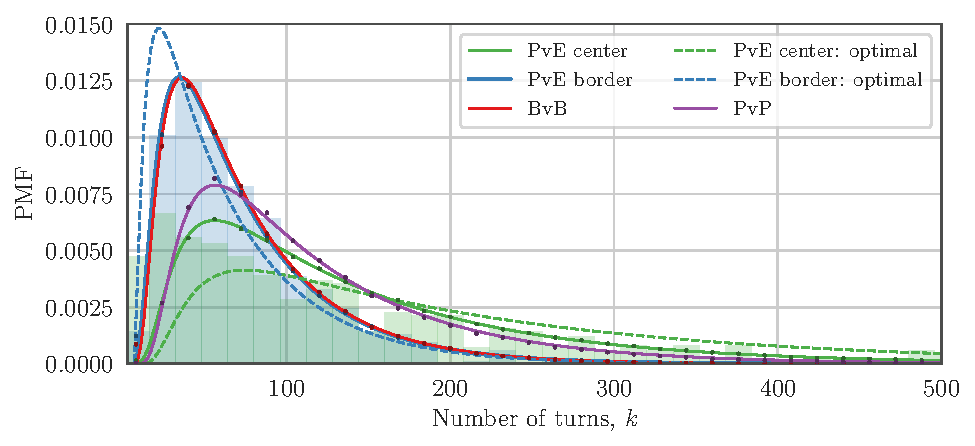
\includegraphics[width=\textwidth,keepaspectratio,clip]{fig3.pdf}
    \caption{
        Распределение количества ходов, полученное моделированием эволюции вероятности (сплошная линия) и численным моделированием (точки) 
        с использованием соответствующих стратегий игроков A и B. 
        Режим BvB (красная линия) представляет собой равновероятный выбор для обоих игроков. Кривые PvE (зеленый и синий) и PvP-режим (фиолетовая линия) 
        были построены на основе соответствующих усредненных стратегий по популяции. Противоположная стратегия в режиме PvE -- это стратегия равновероятного выбора. 
        Оптимальная стратегия для режима PvE в центре (зеленая пунктирная линия) -- держать фишку на диагональной лестнице. Оптимальная стратегия для режима границы PvE 
        (синяя пунктирная линия) -- выбирать движения только вдоль горизонтальной линии. Гистограммы, полученные экспериментально, представлены для режимов PvE 
        (зеленая и синяя области).
    }  
    \label{fig:distribution_time}
    
\end{figure*}

При детальном рассмотрении у всех распределений наблюдаются различия в вероятностях на четных и нечетных ходах. Для оценки характерного поведения распределений, рассмотрим гистограмму с широкими интервалами (длиной в $16$ ходов). Анализ показывает, что все режимы игры следуют одному и тому же паттерну:
\begin{itemize}
\item короткие партии встречаются редко;
\item распределение имеет одну моду с промежуточным числом ходов;
\item вероятность длинных игр экспоненциально уменьшается с увеличением длины игры.
\end{itemize}

Режим PvE за центр демонстрирует аналогичную форму распределения, за исключением того, что мода соответствует коротким играм, которая скрыта при отображении с выбранным размером интервалов.

Хотя количество собранных траекторий в режиме PvP ($500$) не очень большое, в распределении наблюдались нехарактерно долгие игры с длиной более $400$ ходов. 
Вероятность получения таких игр согласно моделированию средней популяционной стратегии ниже $0.015$. 
Однако в играх участников было обнаружено $13$ длинных траекторий в диапазоне от $461$ до $964$ ходов со средним временем поглощения равным $594.27$. 
Обнаруженное отклонение можно объяснить «синхронизацией» между отдельными индивидуумами при длительном взаимодействии. 
Поскольку в среднем один ход занимает $4.5$ секунды, игра с $400$ ходами длится $30$ минут. 
Такое продолжительное время, в течение которого игрок B не может завершить игру, вызывает разочарование и снижает концентрацию, 
что может привести к бессознательному принятию решений, которые может легко предсказать игрок A. 
Потеря концентрации приводит к ухудшению способности человека производить выбор стратегий случайным образом. 
В связи с этим в игре могут возникать процессы «синхронизации».

Подробный анализ этих игр был выполнен путем отделения стратегий этих игр от основной части распределения. 
В результате моделирования столкновения противоположных стратегий для случая PvP 400+ было получено меньшее среднее время поглощения, составившее приблизительно $133.22$ ходов. 
Чтобы сравнить распределения таких игр, также было проведено моделирование эволюции вероятностей для частот, наблюдавшихся в стратегиях длительных игр. 
Соответствующие распределения, полученные для длинных игр, изображены на Рис.~\cref{fig:distribution_time_PvP}. Хотя распределение частот демонстрирует длинный хвост, 
лежащие в основе стратегии, которые появляются в «синхронизированных» играх, не воспроизводят появление столь же длинных игр. 
Таким образом, это демонстрирует наличие зависимости выбора игроков от скрытых факторов, которые нельзя объяснить только свойством цепи Маркова.


\begin{figure*}[t]
    \centering
    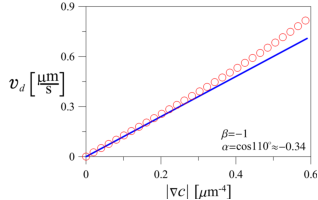
\includegraphics[width=\textwidth,keepaspectratio,clip]{fig4.pdf}
    \caption{
        Распределение времени поглощения для режима PvP (желтая гистограмма и фиолетовая линия) 
        по сравнению с моделированием частот направлений движения (зеленая линия) и частот стратегий (синяя линия), 
        наблюдаемых в длительных играх (более $400$ ходов). Частоты направлений движения для каждого состояния, полученные в 
        экспериментальных длинных играх, использовались для моделирования эволюции вероятностей найти фишку в узлах решетки. 
        Стратегии обоих игроков A и B в PvP с длиной ходов более $400$ использовались отдельно при моделировании.
    }  
    \label{fig:distribution_time_PvP}

\end{figure*}

\subsection{Пространственное распределение}\label{sec:ch3/sec3/sub3}

Затем была проанализирована вероятность нахождения фишки в определенном состоянии во время игры. 
Как и в предыдущих разделах, проведено сравнение экспериментально полученных частот и результатов моделирования. 
Визуализации пространственных распределений для соответствующих стратегий изображены на Рис.~\cref{fig:distribution_states}.

\begin{figure}[t]
    \centering
    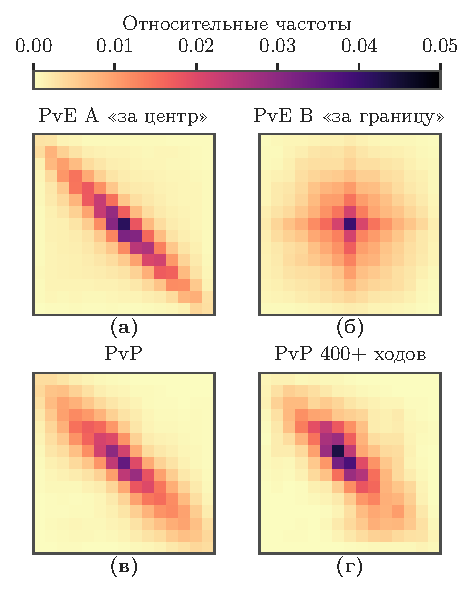
\includegraphics[width=\columnwidth,keepaspectratio,clip]{fig5.pdf}
    \caption{
        Двухмерные распределения частоты посещений узлов решетки, полученные в экспериментальных играх для 4 случаев: 
        PvE за центр, PvE за границу, игры двух игроков (PvP) и игры продолжительностью более $400$ ходов в режиме PvP.
    }  
    \label{fig:distribution_states}
    
\end{figure}

Чистое случайное блуждание демонстрирует дискретное гауссово распределение в пространстве. 
Добавление игровой динамики в свою очередь меняет итоговую картину распределения. 
Как и следовало ожидать, режим PvE в играх за центр демонстрирует в основном движения по диагонали (см. Рис.~\cref{fig:distribution_states}A). 
Хотя это поведение совпадает с пространственным распределением в предложенной оптимальной стратегии, 
экспериментальные данные имеют больший разброс вокруг диагональных состояний, чем для оптимальной стратегии.

Оптимальная стратегия в случае игры PvE за границу демонстрирует вертикальные или горизонтальные линии состояний, 
по которым происходит перемещение фишки. В результате экспериментальных игр PvE за границу найдены 
3 основных паттерна в распределении (см. Рис.~\cref{fig:distribution_states}B): ожидаемые движения по прямым линиям, и 
отличное движение от оптимального паттерна -- это распределение, похожее на чистое случайное блуждание на двумерной квадратной решетке. 
Второй паттерн показывает попытку популяции найти более хорошую стратегию в двумерном пространстве, а не на одномерной линии. 
Однако уход одномерных отрезков увеличивает среднее время поглощения. Это объясняет небольшую разницу в средних временах 
поглощения между экспериментальным играми в случае PvE за границу и чистым случайным блужданием BvB.

Схема пространственного распределения в случае игры PvP (см. Рис.~\cref{fig:distribution_states}C) аналогична случаю PvE при игре за центр: фишка в основном движется по диагонали. Единственное отличие -- увеличенный разброс относительно диагональной линии, который показывает более сильную усредненную стратегию для игрока B, цель которого достичь границу, по сравнению с равновероятным случайным выбором (как в случае игры PvE за центр). Дополнительной характерной особенностью случая PvP является более яркая выраженность блужданий в левой верхней и правой нижней четвертях квадрата относительно центра, в сравнении со случаем PvE при игре за центр. Посещение же двух других четвертей квадрата является более редким событием.

В заключение, было проанализировано пространственное распределение состояний в играх длиной более $400$ ходов. Вероятность расположения фишки в основном сосредоточена на главной диагонали, как и в предыдущих случаях (см. Рис.~\cref{fig:distribution_states}D). Тем не менее, распределение более компактно в центре поля и имеет более высокую вариацию вокруг главной диагонали по сравнению со случаями PvE за центр и PvP. Такое поведение предполагает более длительное нахождение фишки ближе к центру в длинных партиях с движением не только по диагонали, а также перпендикулярно ей.

\subsection{Анализ стратегий}\label{sec:ch3/sec3/sub4}

Далее, рассмотрим сравнение усредненных стратегий популяции для игроков A и B друг с другом, а также с оптимальными стратегиями. Для представления стратегий, визуализируем их в виде цветной двумерной матрицы с элементами, соответствующими состояниям на двумерной квадратной решетке (Рис.~\cref{fig:strategies}). 
Цвет элемента матрицы отображает частоту выбора первой кнопки из двух возможных вариантов в соответствии с правилами (см. Рис.~\cref{fig:controls}). Игрок А, старающийся сохранять фишку внутри поля, имеет два варианта: двигаться вверх/вправо или двигаться вниз/влево; игрок B старающийся как можно скорее достичь границы имеет также два выбора: двигаться вверх/вниз или двигаться влево/вправо. Разные цвета элементов матрицы демонстрируют, какой из двух выборов доминирует для каждого состояния в среднем по всем играм популяции.

\begin{figure*}[t]
    \centering
    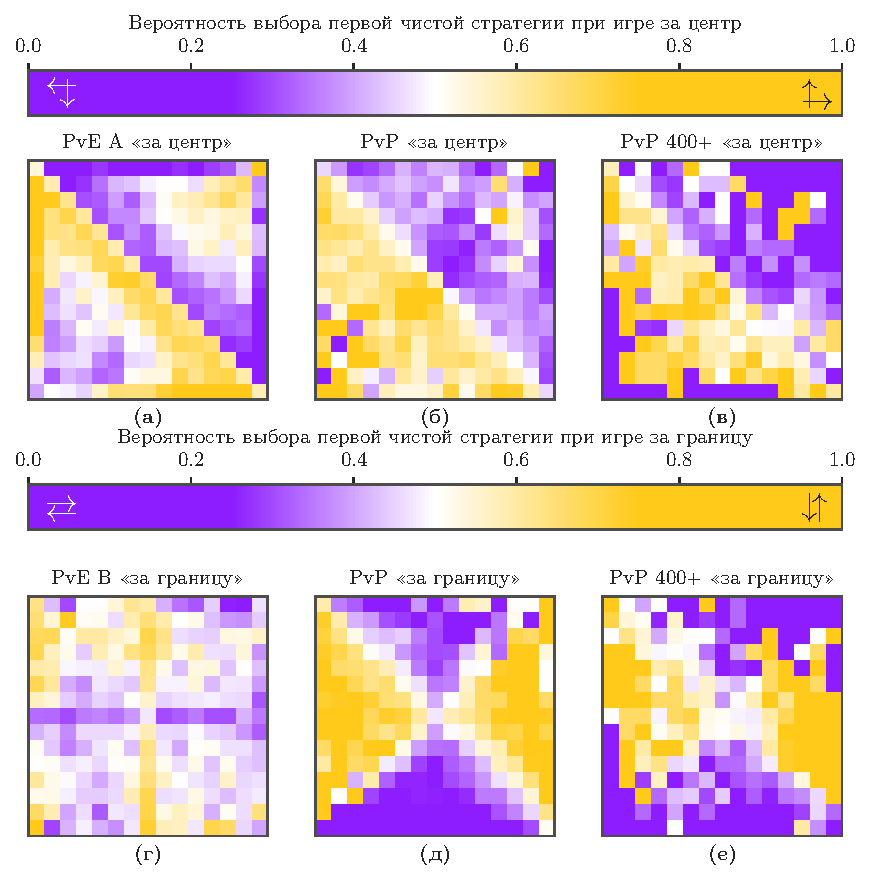
\includegraphics[width=\textwidth,keepaspectratio,clip]{fig6.pdf}
    \caption{
        Визуализация средних популяционных стратегий для разных режимов, полученных в эксперименте. 
        Цвет ячеек отображает частоту выбора первой чистой стратегии: для игры за центр (A, B, C) и для игры за границу (D, E, F).
    }  
    \label{fig:strategies}
    
\end{figure*}

Стратегия, наблюдаемая в случае режима PvE за центр, демонстрирует в основном движение в направлении диагональных состояний (Рис.~\cref{fig:strategies}A). 
Однако состояния, удаленные от диагонали, показывают немного более высокие частоты противоположных стратегий. 
Обычно игроки выбирают уходить от границы, но в состояниях ближе к углам на боковой диагонали поведение становится более случайным 
(относительные частоты ближе к $0.5$). Экспериментальная стратегия на главной диагонали демонстрирует схожесть с первой предполагаемой оптимальной стратегией, 
рассмотренной в разделе \cref{sec:ch3/sec4} <<Решение задачи поиска оптимальных стратегий>>. Напротив, выбор игроков на границе отличается от второй предполагаемой оптимальной стратегии, 
которая предлагает всегда двигаться в направлении от границы. Это приводит к утечке вероятностей за пределы поля не только в углах главной диагонали, 
но и в других пограничных состояниях, что в свою очередь значительно снижает среднее время игры. 

Стратегия игрока играющего за центр в случае PvP аналогична стратегии PvE для игрока за центр (Рис.~\cref{fig:strategies}B). 
Более того, в среднем игроки предпочитают двигаться в направлении главной диагонали независимо от положения на решетке. 
Почти все состояния вблизи границы демонстрируют аналогичную стратегию, за исключением некоторых состояний с почти равной частотой обоих вариантов. 
По сравнению с режимом PvE за центр, игрок в случае PvP играющий за центр имеет немного меньшую уверенность в движении к главной диагонали 
(частоты ближе к $0.5$ в PvP по сравнению с PvE).

Стратегия PvE за границу четко определена на горизонтальной и вертикальной линиях (Рис.~\cref{fig:strategies}D). 
Хотя игроки чаще выбирают движение к ближайшей границе на центральных прямых, частоты в других состояниях не соответствуют общей схеме. 
В отличие от схожих стратегий PvE и PvP в случае игры за центр, стратегия PvP при игре за границу демонстрирует отличающееся поведение с четко прослеживаемым паттерном 
(Рис.~\cref{fig:strategies}E). 
В этом случае игроки действуют прямо противоположно режиму PvE за границу. Усредненная стратегия популяции предлагает выбирать движение 
по координатной линии имеющей наименьшее отклонение от центра. В результате плоскость решений разбивается на $4$ чередующихся треугольника. 
Хотя частоты близки к $0$ или $1$, имеется небольшая разница, которая свидетельствует о редких попытках движения к ближайшей границе.
Такое значительное отличие предположительно связано с очевидностью для игрока за центр выбора оппонента перемещаться в направлении границы.
Это заставляет игрока старающегося достичь границу реже делать попытки перемещения к границе для уменьшения шансов предсказать и противодействовать этому движению
со стороны второго игрока.

Для результирующих стратегий, полученных в длинных играх между двумя игроками (Рис.~\cref{fig:strategies}C,F), 
четких закономерностей не наблюдается из-за ограниченного количества игр. 
Однако наблюдается сходство принципов принятия решений с обычным случаем PvP.


\section{Решение задачи поиска оптимальных стратегий}\label{sec:ch3/sec4}

Предложенная игра Random Walk Game может быть рассмотрена как последовательно составная игра двух оппонентов с нулевой суммой. Конкретизация свойств игры приводит к возможности ее представления в виде рекурсивной игры. На каждом этапе такой игры проводится некоторая игра в нормальной форме из набора доступных игр, в которой стратегии игроков совместно определяют платежи, вероятности каждой из доступных игр на следующем этапе, а также вероятность завершения игры \cite{luce_games_1957a}. В аналогичной форме представляются стохастические игры. Основными особенностями рекурсивных игр по сравнению со стохастическими является возможность наличия нулевых вероятностей завершения игры и произведение платежа только по окончании игры. Анализ рекурсивных игр для общего случая выполнен в работе Эверетта \cite{everett_recursive_1958}.

Представляя игру Random Walk Game в виде рекурсивной игры определим набор доступных простых игр на каждом ходу $\Gamma_{i,j}$, соответствующих внутренним состояниям $(i, j) \in \textbf{S}_{tr}$ на игровом поле. Всего таких простых игр $n^2-4$. Дополнительно определим для индексов, соответствующих поглощающим состояниям марковской цепи, $\Gamma_{i,j}=K, (i,j) \in \textbf{S}_{abs}$, где $K$ обозначает завершение игры с нулевым заключительным платежом. Последовательные вероятности переходов между простыми играми определяются в соответствии с правилами игры Random Walk Game. Тогда матрица для простой игры с индексом $(i, j) \in \textbf{S}_{tr}$ определяется следующим образом:
\begin{equation}
    \begin{aligned}
        \Gamma_{i,j}: \begin{blockarray}{ccc}
     & \mathbin\downarrow\hspace{-0.3em}\uparrow & \text{\makebox[2pt][l]{\raisebox{-5pt}{$\leftarrow$}}}\rightarrow \\
    \begin{block}{l[cc]}
        \text{\makebox[3pt][l]{\raisebox{0pt}{$\uparrow$}}}\text{\makebox[0pt][l]{\raisebox{-7pt}{$\rightarrow$}}} & \Gamma_{i-1,j} & \Gamma_{i,j+1} \\
        \text{\makebox[6pt][l]{\raisebox{6pt}{$\leftarrow$}}}\downarrow & \Gamma_{i+1,j} & \Gamma_{i,j-1} \\
    \end{block}
    \end{blockarray}
    \label{eq:recursive-game-transitions}
    \end{aligned}
\end{equation}
где элементы матрицы определяют переходы из игры, соответствующей состоянию $(i, j)$ в игры, соответствующие состояниям $(i-1, j)$, $(i, j+1)$, $(i+1, j)$, $(i, j-1)$ в исходной марковской цепи; строки матрицы задают стратегии первого игрока, играющего за центр, столбцы матрицы задают стратегии второго игрока, играющего за границу. 

Цена игры $\Gamma_{i,j}^{k}$ на $k$-ом этапе определяется как цена игры на следующем этапе плюс единица, отражающая очередной ход в игре. Тогда для цены игры можно записать:
\begin{equation}
    \begin{aligned}
        |\Gamma_{i,j}^{k}| = 1 + \left | \begin{bmatrix}
			|\Gamma_{i-1,j}^{k+1}| & |\Gamma_{i,j+1}^{k+1}| \\
			|\Gamma_{i+1,j}^{k+1}| & |\Gamma_{i,j-1}^{k+1}|
		\end{bmatrix} \right |
    \label{eq:game-payments}
    \end{aligned}
\end{equation}
где $|\Gamma_{i,j}^k|$ обозначает цену игры $\Gamma_{i,j}$ на $k$-ом этапе.

Обозначим $\nu_{i,j}=|\Gamma_{i,j}|$ цену простой игры $\Gamma_{i,j}$. Тогда каждая простая игра представляет собой матричную игру $2\times2$ с нулевой суммой. Решением такой игры выступает набор смешанных стратегий, если седловая точка отсутствует, иначе -- набор чистых стратегий \cite{ouen_teoriya_1971}. В случае наличия седловой точки в матрице платежей, цена игры равна значению в седловой точке, а стратегии игроков выбираются так, чтобы при их выборе итог игры являлся седловой точкой.
В случае отсутствия седловой точки решением игры выступает набор смешанных стратегий и цена игры может быть найдена по формуле:
\begin{equation}
    \begin{aligned}
        \left | \begin{bmatrix}
			\nu_{i-1,j} & \nu_{i,j+1} \\
			\nu_{i+1,j} & \nu_{i,j-1}
		\end{bmatrix} \right | = \frac{\nu_{i-1,j}\nu_{i,j-1} - \nu_{i+1,j}\nu_{i,j+1}}{\nu_{i-1,j} + \nu_{i,j-1} - \nu_{i+1,j} - \nu_{i,j+1}},
    \label{eq:game-2x2-value}
    \end{aligned}
\end{equation}
при этом вероятности стратегий игроков определяются выражениями:
\begin{equation}
    \begin{aligned}
        p_{i,j}^{(A)} = \frac{\nu_{i,j-1} - \nu_{i+1,j}}{\nu_{i-1,j} + \nu_{i,j-1} - \nu_{i+1,j} - \nu_{i,j+1}}, \\
        p_{i,j}^{(B)} = \frac{\nu_{i,j-1} - \nu_{i,j+1}}{\nu_{i-1,j} + \nu_{i,j-1} - \nu_{i+1,j} - \nu_{i,j+1}}.
    \label{eq:game-2x2-prob}
    \end{aligned}
\end{equation}

Рассматриваемая рекурсивная игра обладает свойством унивалентности \cite{everett_recursive_1958}, то есть имеет неотрицательные (неположительные) платежи в каждой простой игре. Дополнительно игра Random Walk Game не имеет <<ловушек>>, то есть узлов, в которых один из игроков может детерминировано оставлять фишку в течение произвольного числа ходов. В соответствии с работой Эверетта \cite{everett_recursive_1958} и книгой Льюс и Райфа \cite{luce_games_1957a} решением унивалентной рекурсивной игры без <<ловушек>> является одна из неподвижных точек преобразования цен $T$, задающегося как новый вычисленный набор цен игр на основе набора предыдущих цен. Математически преобразование цен $T$ задается следующим образом:
\begin{equation}
    \begin{aligned}
        (\nu_{i,j}) \xrightarrow{T} (\nu_{i,j}^\prime), \\
        \nu_{i,j}^\prime = \big |\Gamma_{i,j} \big(\left (\nu_{i,j} \right ) \big)\big |.
    \end{aligned}
\end{equation}

Для нахождения неподвижной точки преобразования применим численный итеративный метод, многократно применяющий отображение $T$ \cite{everett_recursive_1958}. В качестве начального набора цен выберем произвольный ненулевой вектор $\boldsymbol{\nu}_{init}$ с неотрицательными элементами. 
Итеративно применим отображение $T$ до достижения желаемой точности $\max_{i,j}\left |\nu_{i,j}^{(k)}-\nu_{i,j}^{(k+1)}\right |<\epsilon=10^{-5}$. Заданная точность была достигнута за 1000 итераций. Результирующие значения $\nu_{i,j}$ приведены на рисунке \cref{fig:optimal-value-pvp}.

\begin{figure}[t]
    \centering
    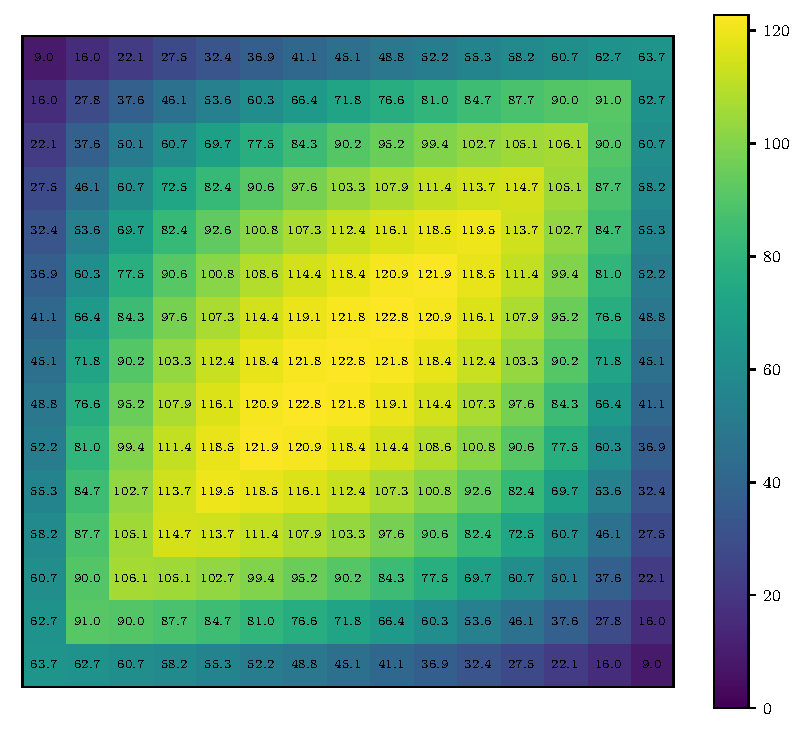
\includegraphics[width=\textwidth,keepaspectratio,clip]{rw-game/pvp_optimal_mean_times.pdf}
    \caption{
        Математическое ожидание числа ходов при оптимальной игре обоих игроков в случае PvP.
    }  
    \label{fig:optimal-value-pvp}
\end{figure}

Применяя формулы \cref{eq:game-2x2-prob} найдем вероятности выбора чистых стратегий в зависимости от положения на поле. Итоговые стратегии игроков при оптимальной игре приведены на рисунках \cref{fig:optimal-strategy-pvp-center,fig:optimal-strategy-pvp-border}. 

\begin{figure}[t]
    \centering
    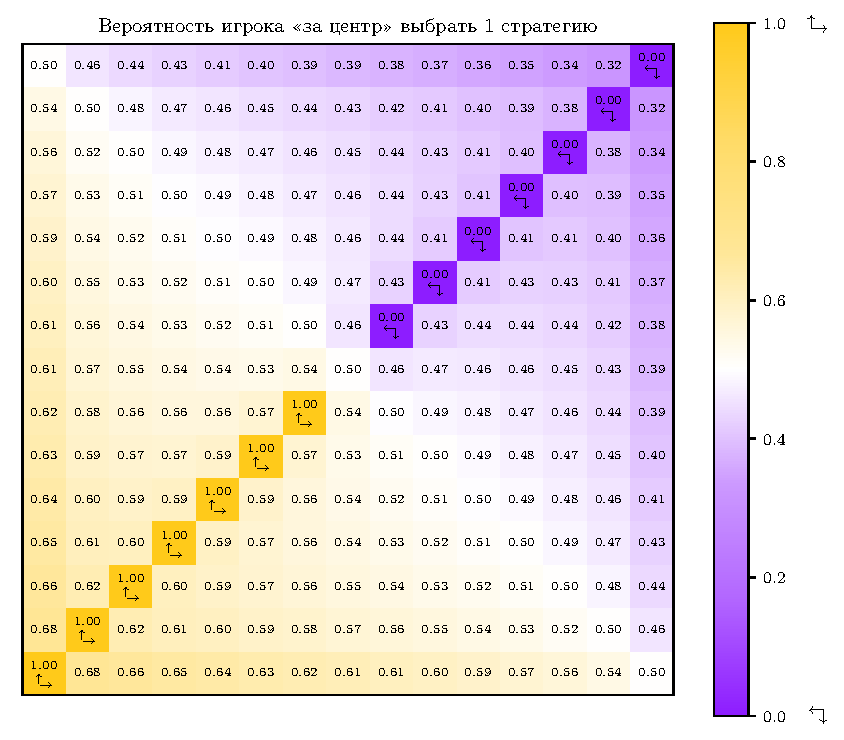
\includegraphics[width=\textwidth,keepaspectratio,clip]{rw-game/pvp_center_strategy.pdf}
    \caption{
        Оптимальная стратегия для игрока за центр в случае PvP.
    }  
    \label{fig:optimal-strategy-pvp-center}
    
\end{figure}

\begin{figure}[t]
    \centering
    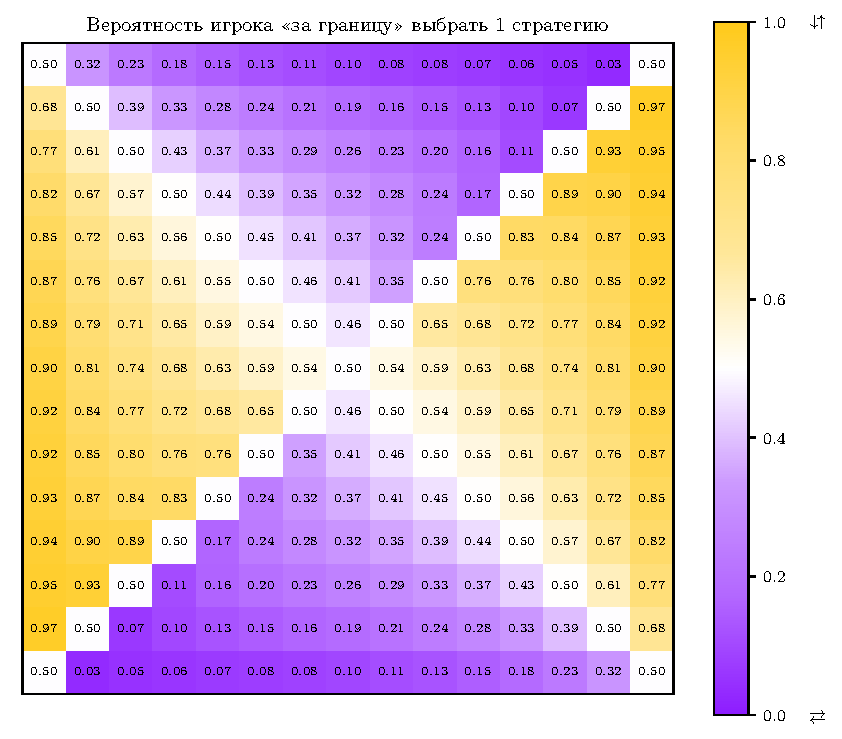
\includegraphics[width=\textwidth,keepaspectratio,clip]{rw-game/pvp_border_strategy.pdf}
    \caption{
        Оптимальная стратегия для игрока за границу в случае PvP.
    }  
    \label{fig:optimal-strategy-pvp-border}
    
\end{figure}

Рассмотрим подробнее получившиеся стратегии игроков. В отсутствии сопротивления от второго игрока, как в случае игры против бота, игрок за центр выбирает кнопку двигающую фишку в сторону диагонали. Находясь выше главной диагонали, соответственно игрок выбирает стратегию движения вниз-влево, а находясь ниже главной диагонали -- вверх-вправо. Добавление же второго игрока, оптимизирующего свою стратегию, заставляет первого игрока видоизменить свою стратегию, существенно уменьшив вероятности движения в сторону главной диагонали. Так, средняя вероятность выбора стратегии движения к главной диагонали, за исключением побочной диагонали, составляет всего $\approx 0.56$. Максимальная вероятность выбора стратегии движения к главной диагонали за исключением побочной диагонали, достигается в граничных узлах соседних с угловыми узлами побочной диагонали и составляет $\approx 0.68$. При удалении фишки от главной диагонали игрок за центр плавно увеличивает вероятность движения в сторону главной диагонали, при этом соотношение выбора стратегий изменяется от $1:1$ на главной диагонали до соотношения $\approx 3:2$ в пользу движения к главной диагонали. Выбор движения в центральном узле и на главной диагонали для игрока за центр не имеет значения, так как переходы из этих узлов приводят к симметричным играм. Движение же на побочной диагонали строго определено и должно осуществляться в направлении главной диагонали. Таким образом, стратегия игрока за центр интуитивно соответствует цели <<движения от границы>> с учетом большей рандомизации ходов.

Стратегии игрока за границу в сравнении с оптимальными стратегиями при игре против бота, напротив, имеют существенные различия. При игре против бота игрок за границу выбирает одно из направлений вертикальное или горизонтальное и всегда выбирает стратегию движения вдоль этого направления, никогда не пытаясь выбирать перпендикулярное направление параллельно ближайшей границе. Добавление в игру оппонента, оптимизирующего свою стратегию, игрок за границу попадает в ситуацию необходимости не демонстрировать свое намерение двигаться к границе, что заставляет его чаще выбирать движение параллельно ближайшей границе. Так средняя вероятность движения параллельно ближайшей границе за исключением побочной и главной диагоналей составляет $\approx 0.74$. Вблизи граничных узлов средняя вероятность достигает $\approx 0.87$, а максимальная вероятность $\approx 0.97$. Таким образом стратегия игрока за границу состоит в плавном увеличении вероятности движения параллельно ближайшей границе по мере приближения к ней. 


\section{Оценка когнитивного статуса при возрастных изменениях}\label{sec:ch3/sec5}

\section{Выводы по главе 3}\label{sec:ch3/sec6}

В данной главе были рассмотрены основные результаты сравнения статистических свойств экспериментально
полученных траекторий и стратегий игроков с соответствующими результатами моделирования различными подходами. 
Предложена гипотеза об оптимальных средних временах достижения границы для двух случаев игры и 
рассмотрены соответствующие стратегии, достигающие оптимальных времен. Продемонстрирована оптимальность
данных стратегий и средних времен игры для случаев малого размера поля.
В главе для анализа игры Random Walk Game применены подходы численного моделирования, моделирования эволюции вероятности и полевого эксперимента,
на основе которых вычислены средние времена игры, распределения времен игры и пространственные распределения фишки на поле. 
Полученные результаты визуализированы с использованием языка Python 3.8 и библиотек numpy, scipy, matplotlib.

% \section{Выводы по главе 2}\label{sec:ch2/sec4}

% В данной главе были рассмотрены алгоритмы и методы исследования, примененные для анализа 
% предложенной игры в терминах Марковских процессов. Получено описание игрового процесса 
% с использованием аппарата поглощающих Марковских цепей и смешанных стратегий. В главе представлены
% подходы численного моделирования, моделирования эволюции вероятности и полевого эксперимента, 
% примененные к анализу игры Random Walk Game. Представление стратегий игроков сведено к двум многомерным вещественным векторам с учетом двух целей.
% Предложенные методы реализованы с использованием языка Python 3.8 и библиотек numpy, scipy, matplotlib.
% Разработано и реализовано мобильное приложение для игры Random Walk Game на базе технологии Xamarin
% для операционных систем Android и iOS. 
           % Глава 3
\chapter*{Заключение}                       % Заголовок
\addcontentsline{toc}{chapter}{Заключение}  % Добавляем его в оглавление

%% Согласно ГОСТ Р 7.0.11-2011:
%% 5.3.3 В заключении диссертации излагают итоги выполненного исследования, рекомендации, перспективы дальнейшей разработки темы.
%% 9.2.3 В заключении автореферата диссертации излагают итоги данного исследования, рекомендации и перспективы дальнейшей разработки темы.
%% Поэтому имеет смысл сделать эту часть общей и загрузить из одного файла в автореферат и в диссертацию:

В диссертационном исследовании получены следующие результаты.
%% Согласно ГОСТ Р 7.0.11-2011:
%% 5.3.3 В заключении диссертации излагают итоги выполненного исследования, рекомендации, перспективы дальнейшей разработки темы.
%% 9.2.3 В заключении автореферата диссертации излагают итоги данного исследования, рекомендации и перспективы дальнейшей разработки темы.
\begin{enumerate}
  \item Построена стохастическая модель генерации степенных распределений длительностей нахождения системы в одном из двух состояний за счет дробового шума. Получен способ оценки распределения длительностей для модели. Найдены параметры для генерации двух чередующихся режимов: степенное распределение и экспоненциальное распределение длительностей.
  \item Получена аналитическая форма средней скорости колонии бактерий в случае паттерна движения с двумя чередующимися углами. Проведенный численный эксперимент позволил подтвердить корректность формулы при малом химическом градиенте, а также продемонстрировать наличие отклонений при большом градиенте. 
  \item Получена оценка параметров химической чувствительности бактерий и коэффициента диффузии при их движении в условиях нелинейной радиальной концентрации химического вещества с применением численного эксперимента.
  \item Построена стохастическая модель, описывающая предложенный игровой конфликт двух игроков, управляющих блужданием фишки на конечной квадратной решетке. 
  \item Разработаны методы для расчета статистических характеристик игрового процесса при фиксированных заданных стратегиях игроков, таких как среднее время игры, распределение времен игры, распределение вероятностей наблюдения фишки в состояниях конечной решетки. 
  \item Вычислены оптимальные средние времена для трех случаев игры, предложены классы оптимальных стратегий и визуализированы конкретные стратегии. Предложен подход для нахождения оптимальных стратегий при произвольной стратегии оппонента, а также при оптимальной стратегии.
  \item Разработано мобильное приложение Random Walk Game, реализующее игровую механику посредством сети интернет с использованием созданного веб-сервера по обработке и хранению результатов игр участников. Дополнительно разработан веб-сайт для отображения статистической информации по результатам игр участников в режиме реального времени. Приложение опубликовано в открытом доступе на двух маркетплейсах для платформ Android и iOS.
  \item Проведен масштабный эксперимент с применением мобильных и интернет-технологий, привлекший более 100 участников и позволивший собрать более 1500 игр Random Walk Game. 
  \item Подтверждено соответствие эксперимента предложенной модели для трех случаев игры на основе сравнения распределений и соответствующих средних времен игры. 
  \item Установлены возникающие особенности синхронизации игроков при длительных играх, связанные со снижением концентрации игроков. Длительные игры утомляют игроков, что снижает способность человека генерировать чисто случайную последовательность выборов.
  \item Выявлены отличия стратегий игроков от оптимальных стратегий на основе сравнения статистических свойств траекторий и стратегий участников для случаев игры против стратегии равновероятного случайного выбора.
\end{enumerate}


Дальнейшие исследования могут быть связаны с поиском квазистационарных состояний, возникающих в поглощающих Марковских цепях. Отдельный интерес представляет измерение уровня синхронизации между игроками, изменяющегося в течение игры. Необходимой составляющей для проведения такого типа анализа является возможность получения большего числа длительных игр между игроками, что позволит выявить причины возникновения корреляции между решениями участников на каждом ходу. Построенная в данной работе стохастическая модель игры и реализация мобильного могут быть использованы другими исследователями теории игр, как отправная точка для построения игр, обладающих свойством описания решений участников популяции и воспроизведения их поведения в модели. 

В заключение автор выражает благодарность и большую признательность профессору Денисову~С.\,В. за поддержку, помощь, обсуждение результатов, прямое участие в игровом процессе, за предложенную идею, за помощь в разработке дизайна игры, и~научное руководство. Также автор благодарит Иванченко~М.\,В. за поддержку, помощь в организации процесса подготовки диссертации, Тихомирова~С.\,Н. за помощь в~анализе игр, помощь в разработке мобильного приложения, помощь в организации мероприятий и поиске участников, Карчкова~Д.\,А. за предоставленный экскурс в разработку кроссплатформенных мобильных приложений, Забурдаева~В.\,Ю. за~постановку задач в области хемотаксиса и помощь в применении аналитического аппарата при исследовании хемотаксиса, Полевую~С.А. за разработанные когнитивные тесты, Кондакову~Е.В. за подготовку выборки результатов прохождения когнитивных тестов, и авторов шаблона *Russian-Phd-LaTeX-Dissertation-Template* за~помощь в оформлении диссертации. Автор также благодарит всех участников игрового эксперимента и~всех, кто сделал настоящую работу автора возможной.
      % Заключение
\printnomenclature[3.5cm] % Значение ширины столбца с обозначениями стоит подбирать вручную

\textbf{БД} : База данных

\textbf{PvE} : Player vs Environment
\textbf{PvP} : Player vs Player
\textbf{BvB} : Bot vs Bot
\textbf{REST} : Representational state transfer 
\textbf{API} : Application Programming Interface
\textbf{API} : Application Programming Interface
        % Список сокращений и условных обозначений
\chapter*{Словарь терминов}             % Заголовок
\addcontentsline{toc}{chapter}{Словарь терминов}  % Добавляем его в оглавление

\textbf{Случайный процесс} : Семейство случайных величин, индексированных некоторым параметром, играющим роль времени.

\textbf{Случайное блуждание} : Случайный процесс, описывающий путь, состоящий из последовательности случайных шагов в математическом пространстве.

\textbf{Цепь Маркова} : Последовательность случайных событий с конечным или счетным числом исходов, где вероятность наступления каждого события зависит только от состояния, достигнутого в предыдущем событии

\textbf{Двудольный граф} : Граф, множество вершин которого можно разбить на две части таким образом, 
что каждое ребро графа соединяет вершину из одной части с какой-то вершиной другой части, то есть не существует рёбер между вершинами одной и той же части графа.

\textbf{Антагонистические игры} : Некооперативная игра, в которой участвуют два или более игроков, выигрыши которых противоположны.

\textbf{Некооперативная игра} : Математическая модель взаимодействия нескольких сторон (игроков), в процессе которого они не могут формировать коалиции и координировать свои действия.

\textbf{Матрица Теплица} : Матрица, в которой на всех диагоналях, параллельных главной, стоят равные элементы.

      % Словарь терминов
\include{Dissertation/references}      % Список литературы
\include{Dissertation/lists}           % Списки таблиц и изображений (иллюстративный материал)

\setcounter{totalchapter}{\value{chapter}} % Подсчёт количества глав

%%% Настройки для приложений
\appendix
% Оформление заголовков приложений ближе к ГОСТ:
\setlength{\midchapskip}{20pt}
\renewcommand*{\afterchapternum}{\par\nobreak\vskip \midchapskip}
\renewcommand\thechapter{\Asbuk{chapter}} % Чтобы приложения русскими буквами нумеровались

%\include{Dissertation/appendix}        % Приложения

\setcounter{totalappendix}{\value{chapter}} % Подсчёт количества приложений

\end{document}
